\documentclass[11pt,a4paper]{article}
\usepackage[margin=2.0cm,headsep=0.5cm,headheight=14pt]{geometry}
\usepackage[T1]{fontenc}
\usepackage[utf8]{inputenc}
\usepackage{amsmath,amssymb,lmodern,microtype,booktabs,longtable,array,xcolor,enumitem,tikz,pgfplots,tcolorbox,fancyhdr,titlesec,graphicx,float,ragged2e,multicol,needspace,pdflscape,textcomp}
\usepackage[colorlinks=true,linkcolor=acc,urlcolor=acc,citecolor=acc]{hyperref}
\usepackage{url}
\pgfplotsset{compat=1.16}
\usetikzlibrary{arrows.meta,positioning,shapes.geometric,calc,fit,decorations.pathmorphing}
\definecolor{acc}{HTML}{1F4E79}\definecolor{ok}{HTML}{2E7D32}\definecolor{warn}{HTML}{B26A00}\definecolor{bad}{HTML}{B3261E}\definecolor{mid}{HTML}{5A5A5A}
\titleformat{\section}{\Large\bfseries\color{acc}}{\thesection}{0.6em}{}
\titleformat{\subsection}{\large\bfseries\color{acc}}{\thesubsection}{0.5em}{}
\titleformat{\subsubsection}{\normalsize\bfseries\color{acc}}{\thesubsubsection}{0.5em}{}
\setlist{itemsep=2pt,topsep=3pt}
\pagestyle{fancy}\fancyhf{}\fancyfoot[C]{\thepage}\fancyhead[L]{\small C001 quirks: theory track}\fancyhead[R]{\small Report, 8 Oct 2026}
\fancypagestyle{lscape}{\fancyhf{}\fancyfoot[C]{\thepage}}
\renewcommand{\arraystretch}{1.12}
\setlength{\tabcolsep}{4pt}
\setlength{\emergencystretch}{3em}
\renewcommand{\topfraction}{0.9}\renewcommand{\bottomfraction}{0.8}\renewcommand{\textfraction}{0.07}\renewcommand{\floatpagefraction}{0.7}
\setlength{\LTcapwidth}{\textwidth}\setlength{\LTpre}{4pt}\setlength{\LTpost}{6pt}
\newtcolorbox{key}[1][]{colback=acc!6,colframe=acc,boxrule=0.6pt,arc=2pt,left=6pt,right=6pt,top=4pt,bottom=4pt,#1}
\tcbuselibrary{breakable}
\newtcolorbox{caution}[1][]{breakable,colback=warn!8,colframe=warn,boxrule=0.6pt,arc=2pt,left=6pt,right=6pt,top=4pt,bottom=4pt,#1}
\newtcolorbox{good}[1][]{colback=ok!6,colframe=ok,boxrule=0.6pt,arc=2pt,left=6pt,right=6pt,top=4pt,bottom=4pt,#1}
\newcolumntype{L}[1]{>{\RaggedRight\arraybackslash}p{#1}}
\newcolumntype{C}[1]{>{\centering\arraybackslash}p{#1}}
% ---- macros
\newcommand{\arx}[1]{\href{https://arxiv.org/abs/#1}{arXiv:#1}}
\newcommand{\ax}[1]{\href{https://arxiv.org/abs/#1}{#1}}
\newcommand{\EST}{\textsc{estimate}}
\newcommand{\UNV}{\textsc{unverified}}
\newcommand{\VER}{\textsc{verified}}
\newcommand{\WD}{\textcolor{bad}{\textsc{withdrawn}}}
\DeclareRobustCommand{\file}[1]{\path{#1}}
\newcommand{\mQ}{m_Q}
\newcommand{\NIC}{N_{\mathrm{IC}}}
\newcommand{\GeV}{\ensuremath{\,\mathrm{GeV}}}
\newcommand{\TeV}{\ensuremath{\,\mathrm{TeV}}}
\newcommand{\keV}{\ensuremath{\,\mathrm{keV}}}
\newcommand{\MeV}{\ensuremath{\,\mathrm{MeV}}}
\newcommand{\fb}{\ensuremath{\,\mathrm{fb}}}
\newcommand{\pb}{\ensuremath{\,\mathrm{pb}}}
\newcommand{\fbinv}{\ensuremath{\,\mathrm{fb}^{-1}}}
\newcommand{\abinv}{\ensuremath{\,\mathrm{ab}^{-1}}}
\newcommand{\QQ}{Q\bar Q}
\newcommand{\pTQQ}{p_T(Q\bar Q)}
\newcommand{\ns}{\ensuremath{\,\mathrm{ns}}}
\newcommand{\um}{\ensuremath{\,\mu\mathrm{m}}}
\newcommand{\mus}{\ensuremath{\,\mu\mathrm{s}}}
\newcommand{\gst}{\gamma^*}
\newcommand{\lmax}{\ell_{\max}}
\newcommand{\Ds}{\Delta s}
\newcommand{\sqs}{\sqrt{\sigma}}
\newcommand{\catA}{\textcolor{bad}{\textbf{A}}}
\newcommand{\catB}{\textcolor{warn}{\textbf{B}}}
\newcommand{\catC}{\textcolor{mid}{\textbf{C}}}
\newcommand{\lab}[1]{\textbf{[#1]}}
\newcommand{\src}[1]{{\color{mid}[#1]}}
\newcommand{\EXPL}{\textcolor{ok}{\textbf{EXPLOIT}}}
\newcommand{\WAC}{\textcolor{warn}{\textbf{WORTH A CHECK}}}
\newcommand{\NAG}{\textcolor{bad}{\textbf{NOT A GAP}}}

\begin{document}
\begin{titlepage}
\centering\vspace*{2.0cm}
{\Huge\bfseries\color{acc} Colour-neutral quirks:\\[6pt] the theory track}\\[0.9cm]
{\Large Candidate C001, Stage 2 (parallel to Phase 2):\\[3pt] gaps in quirk theory that a CMS search can exploit,\\[3pt] discrepancies in the literature and in public code,\\[3pt] and four rounds of independent review}\\[1.2cm]
{\large Report on the theory-track work}\\[0.5cm]
{\large 8 October 2026}\\[1.3cm]
\begin{minipage}{0.86\textwidth}\small
\begin{key}
\textbf{Status: final.} Authoritative source: \file{theory_track/outputs/THEORY_GAPS_SYNTHESIS.md}, \textbf{version~4} (``v4''). Review loop: \textbf{R1} critical + constructive \textcolor{warn}{ITERATE} $\to$ \textbf{R2} \textcolor{warn}{ITERATE} $\to$ \textbf{R3} \textcolor{warn}{ITERATE} (literature credit only) $\to$ \textbf{R4} \textcolor{ok}{\textbf{PASS}} (0\,A, 0\,B, 7\,C; C items applied).\\[3pt]
\textbf{No new exclusion was derived by this track.} The results are corrections to the signal model and to the search window, a validated production propagator, a measurement method for $(\mQ,\Lambda)$ after a discovery, reach \emph{projections} for complementary channels, and readings of existing limits.\\[3pt]
\textbf{Nothing outside \file{theory_track/} was edited.} Every proposed change to the project documents (Section~\ref{sec:mods}) awaits a decision by the user.
\end{key}
\vspace{4pt}
\textbf{Benchmark:} $E=(1,1)_{-1}$ vector-like Dirac fermion quirk, $\NIC=2$, $\Lambda\equiv\sqs$ (string tension $\sigma$), Drell--Yan production; CMS Phase-2 (3.8\,T, PU 200, $3\abinv$), with Run~3 noted where results differ.\\[3pt]
\textbf{Workspace:} \file{hllhc_search/stage2_C001_quirks/theory_track/}. Methodology: a JFC-style loop (JFC is the project's analysis methodology: each phase ends in a written artifact that independent reviewers check before the next phase); here parallel investigators $\to$ synthesis $\to$ independent review $\to$ fix $\to$ fresh reviewer.\\[3pt]
\textbf{Labels:} \EST{} = our own calculation (script named); \UNV{} = recalled, secondary, or a by-eye figure reading, not checked against the primary source; \VER{} = checked by independent code or a closed form. Source tags: \src{S-n} ranked gap of the synthesis, \src{T3 \S3.2} investigator report section, \src{R1} reviewer code, \src{1911.02223 Eq.III.12} primary paper.
\end{minipage}
\vfill
{\small Prepared for the USFQ CMS group. Written by the report agent W from the theory-track files; where an investigator report disagrees with synthesis v4, v4 is followed.}
\end{titlepage}

% ======================================================================
\section*{Executive summary}
\addcontentsline{toc}{section}{Executive summary}
\vspace{-4pt}
{\small
\begin{key}
\textbf{Bottom line.} The theory track did not derive a new exclusion. It found that the projected mass reach of the coplanar tracker search ($\approx1.1$--$1.2\TeV$, STRATEGY \S6.1) is not changed at a level we can compute, but that several numbers and recipes in the project's strategy and signal model are wrong or need qualification, and it delivered a propagator that is now validated against an independent solver. The fastest route to a \emph{stronger} limit is an update of Evans and Luty's existing recast \cite{EvansLuty} of the CMS stopped-particle search with full Run-2+3 data and a causal-string stopping fraction: $\mQ\approx0.15$--$0.35\TeV$ (\EST{}), which would beat FASER and D0 at $\Lambda\lesssim1.5\keV$ (and, extrapolated, near 100\,keV) even with a 2016-like background, judged against FASER's HEPData limits \src{S-8; Section~\ref{sec:stopped}}.\\[2pt]
{\footnotesize Acronyms (IT/OT, PS/2S, BTL/MTD, PU, HSCP, MET, SBI, CRB, JFC, \ldots) and symbols ($\Lambda$, $\gst$, $\ell_0$, $\Ds$) are defined in the glossary, Appendix~\ref{app:gloss}.}
\end{key}

\textbf{1.\ The confinement scale $\Lambda$} \src{Box A, S-11, S-15}.
\begin{itemize}[leftmargin=1.2em,itemsep=0pt,topsep=1pt]
\item \emph{Convention.} The cosmology paper \cite{cool} uses $\Lambda=T_c$ with $T_c=0.6\sqs$ (the $N\to\infty$ value). For SU(2) the lattice gives $T_c/\sqs=0.709$, so its ``1\,keV'' is $\sqs=1.41\keV$. Our own \file{theory_signal_model.md} uses $1/0.6$, which is 18\% off \src{T1 G-T1-1; \VER{}, S check 5}.
\item \emph{Where the tracker is sensitive.} Truth-level 50\% edge of the $\Ds<100\um$ finder at $\Lambda_{\rm low}\approx0.45$--$0.7\keV$ (200--1000\,GeV), up to $\approx20$--$30\keV$ where the pair merges. With realistic hit resolution the edge is \emph{undefined} until the cut is set at fixed background efficiency \src{S-2, S-3}.
\item \emph{Existing limits} on the $E$ singlet: nothing above $\approx0.18\TeV$ in 0.3--100\,keV (FASER, D0); Farina--Low exclude 0.15--0.65\,TeV only at $\Lambda\le0.1\keV$ \src{Box A}.
\item \emph{Priors and cosmology.} The only UV framework that predicts $\Lambda$ in the window (SUSY-GUT ladder) predicts \emph{doublets}, which are invisible to the tracker \src{S-14}. A discovery would imply $T_{\rm RH}\lesssim5$--$40\GeV$ (the implication itself is from \cite{cool}; the window numbers, the SU(2) conversion and the $T_{\rm RH}^{21/4}$ scaling are ours) \src{S-15}.
\end{itemize}

\textbf{2.\ Oscillation length} \src{Box B}. Exact closed forms: $\lmax=3.95\,{\rm cm}\,(\gst-1)(\mQ/100\GeV)(\keV/\Lambda)^2$ and $N_{\rm osc}\approx12(\Lambda/\keV)^2$ in the CMS tracker, \emph{independent of $\mQ$} (\VER{}). The literature shorthand ``1\,cm$(m/100\GeV)(\keV/\Lambda)^2$'' is wrong by $\times0.4$--2.7 event by event. Scalars: $\lmax\times1.7$, $N_{\rm osc}\times0.81$. A fixed-$p_T$ ISR kick biases $\lmax$ by $-10$ to $-25\%$.

\textbf{3.\ Propagation dynamics} \src{S-1, S-2, S-3, S-6, S-8, S-10}.
\begin{itemize}[leftmargin=1.2em,itemsep=0pt,topsep=1pt]
\item The \emph{causal string} (the ATLAS Athena algorithm; our port \file{code/T3_causal.py}) is exact classical Nambu--Goto: an independent conformal-gauge solver agrees to 0.990--1.004 in plane thickness (\VER{}, R1).
\item The \emph{Li method} (CM-simultaneous straight string \cite{LiLi,traj}) is a good approximation only when step-converged; its thickness deficit depends on $\gst$: $\approx3\%$ low at $\gst\approx1.05$, $\approx15\%$ at the median $\gst\approx1.3$, 30--35\% at $\gst=2$--3 (single events $-47\%\ldots+36\%$; $\Lambda$-independence tested only at $\gst=1.28$, the $\gst$ dependence only at 1\,keV). At the step bound printed in the paper the Euler integration is not converged ($\times0.8$--20 in thickness).
\item A \emph{lab-time-slice} straight string is badly wrong ($\times1.5$--75). The v1 headline ``published models are wrong at O(1)'' was based on this stand-in and is \WD{}.
\item Multiple scattering sets a truth-level thickness floor of 11/15/22\um\ (200/500/1000\,GeV; material per layer \UNV{}). The B-field thickness scales as $\Lambda^{-1.6\ldots-2.0}$, roughly $\mQ$-independent (qualitatively already in Li et al.\ \cite{traj}), and is non-linear in $B$ through a $B\ln(1/B)$ effect at near-miss crossings (new; \VER{}).
\item Timing: median delays at the timing layer 3.5/9.6/18.7\,ns, for the real triggered spectrum; the strategy's 6/16/33\,ns are medians at a fixed $\pTQQ=250\GeV$, which coincide with the 84th percentiles (6.2/16.5/32.8\,ns) of the real spectrum. Merged pairs deposit 9--21$\times$ MIP, not $2\times$.
\end{itemize}

\textbf{4.\ Trajectory model} \src{S-4, S-5, S-7}.
\begin{itemize}[leftmargin=1.2em,itemsep=0pt,topsep=1pt]
\item \emph{Degeneracy theorem:} hits, hit times and dE/dx depend on $(\mQ,\Lambda)$ only through $\ell_0=\mQ/\sigma$ and the velocities. $\mQ$ needs the MET recoil: $\approx1$--3\% on $\mQ$ and 0.5--1.5\% on $\Lambda$ with 30 events, MET-scale limited (\EST{}, idealised).
\item MET-strip alignment rejects \emph{random} planes $\times13$--34 at 95\% signal efficiency (quantifies a cut proposed by Knapen et al.); the gain on real backgrounds is unknown.
\item With realistic resolution the coplanarity test is carried by the Inner Tracker (per-hit out-of-plane $\sigma_n\approx17\um$ IT, 0.25\,mm PS, 8\,mm 2S).
\end{itemize}

\textbf{Other exploitable gaps:} the Athena \texttt{MaxSteps}$=2\times10^6$ step killer that would stop quirks for $\Lambda\gtrsim24\keV$ in a CMS-size tracker (do first) \src{S-9}; a doublet monojet recast \src{S-14}; $|q|=2$ singlets \src{S-17}.

\textbf{Discrepancies} (Section~\ref{sec:disc}): $\Lambda$ conventions; $\Omega\propto T_{\rm RH}^7$ vs $T_{\rm RH}^{21/4}$ and a $\times2.2$ in \cite{cool}; Li et al.'s unconverged printed step; \cite{LiPei} \S5 not supported by the degeneracy theorem; a 37\% Knapen--Li reach difference; the Athena step killer; several numbers in our own strategy; our own earlier errors (separate box).

\textbf{Key numbers} (status in brackets; details in the sections cited):\\[1pt]
{\footnotesize\begin{tabular}{@{}L{5.6cm}L{8.2cm}L{2.6cm}@{}}\toprule
Quantity & Value & Where\\\midrule
Causal string vs independent NG solver & thickness ratio 0.990--1.004 (\VER{}) & S-1, Tab.~\ref{tab:S1}\\
Converged Li method / causal & 0.97 / 0.85 / 0.65--0.69 at $\gst$ = 1.05 / 1.3 / 2--3 (\VER{}) & S-1\\
Window lower edge (50\%, truth level) & $\Lambda_{\rm low}\approx0.45$--0.7\,keV (\EST{}) & S-3\\
MS thickness floor (truth level) & 11/15/22\um\ at 200/500/1000\,GeV (\EST{}, material \UNV{}) & S-2\\
Median BTL delay & 3.5/9.6/18.7\,ns at 200/500/1000\,GeV (\VER{}) & S-6\\
$(\mQ,\Lambda)$ after discovery, 30 events & 1--3\% / 0.5--1.5\% (\EST{}, idealised) & S-4\\
Run-2+3 stopped-pair update & 0.15--0.35\,TeV; above FASER/D0 at $\Lambda\lesssim1.5\keV$ with $B\approx80$ (\EST{}) & S-8, \S\ref{sec:stopped}\\
\bottomrule\end{tabular}}

\textbf{Decisions for the user} (Section~\ref{sec:decisions}): apply the document changes; hand \file{T3_causal.py} to Phase~2; launch the Run-2+3 stopped-pair update; pull the Phase-2 material budget; contact code authors.
}

\newpage
{\setcounter{tocdepth}{2}\tableofcontents}
\clearpage

% ======================================================================
\section{Reading guide: important files to read}\label{sec:reading}
This report is a curated, self-contained summary. The Markdown files are the record; when in doubt, \textbf{synthesis v4 wins} over the investigator reports, and the investigator reports win over this report on details. All paths below are relative to \file{stage2_C001_quirks/theory_track/} unless they start with \file{../}. Priority: \textbf{1} = read first; \textbf{2} = read when acting on that topic; \textbf{3} = reference or audit trail.

\subsection{Files, in recommended order}
{\small
\begin{longtable}{@{}L{4.6cm}L{6.0cm}L{4.3cm}C{0.9cm}@{}}
\caption{Important files of the theory track. Sizes on disk on 8 Oct 2026.}\label{tab:files}\\
\toprule File & What it contains & Why / when to read it & Prio.\\\midrule\endfirsthead
\toprule File & What it contains & Why / when to read it & Prio.\\\midrule\endhead
\bottomrule\endfoot
\multicolumn{4}{@{}l}{\textit{Synthesis (authoritative)}}\\*
\file{outputs/THEORY_GAPS_SYNTHESIS.md} (v4, 148\,kB, 1078 lines) & Glossary and executive summary by the four requested topics (\S0); Box~A ($\Lambda$), Box~B (oscillation length), ranked gaps S-1\ldots S-20 (\S1); cross-report tensions X-1\ldots X-13 (\S2); 23 spot checks (\S3); recommended edits to the project documents by file and section (\S4); recasts (\S4.5); Run~3 vs Phase~2 (\S4.6); publishable outputs (\S5); killed ideas (\S6); unverified items (\S7); next steps (\S8); responses to all reviews (\S10) & always. Start with \S0, then \S1 table, \S4, \S5, \S8 & \textbf{1}\\
\file{outputs/THEORY_GAPS_SYNTHESIS_v1.md}, \file{_v2.md}, \file{_v3.md} & Earlier versions, unchanged. v1 contains the \WD{} S-1 headline & only to audit how a claim changed & 3\\
\midrule
\multicolumn{4}{@{}l}{\textit{Investigator reports (one per workstream)}}\\*
\file{investigations/T1_lambda.md} (29\,kB) & $\Lambda$ conventions (lattice table), SUSY-GUT ladder, naturalness prior, cosmology (thermal history, freeze-in $T_{\rm RH}$ bound), astro/collider indirect probes & before quoting any $\Lambda$ conversion or a cosmology statement & 2\\
\file{investigations/T2_string_dynamics.md} (53\,kB) & Exact vacuum solution and closed forms ($\lmax$, $N_{\rm osc}$), DY distributions, angular momentum, crossings, semiclassics, the Athena code review (\S5.1), MaxSteps killer (G-T2-2). \textbf{Carries an erratum box}: all labSS/cmSS numbers marked ``superseded'' & oscillation-length questions; Athena code details. Ignore the superseded labSS numbers & 2\\
\file{investigations/T3_propagation.md} (56\,kB) & Phase-2 material model (\S2), causal-string thickness with/without MS (\S3.2), precession (\S4), net-charged pairs (\S5), timing (\S6), $f_{\rm stop}$ (\S7), dE/dx (\S8), revised window (\S9). \textbf{Carries an erratum box} (straight-string-with-MS statements; truth level) & thickness, timing, stopping numbers; the material assumptions & 1\\
\file{investigations/T4_trajectory_model.md} (51\,kB) & 9-parameter causal fit model, degeneracy theorem, Fisher/Cram\'er--Rao, B as $\Lambda$ meter, MET alignment, seeding, L1 stubs, energy-loss phase drift & measurement after discovery; reconstruction design & 2\\
\file{investigations/T5_literature_audit.md} (70\,kB) & INSPIRE census (484 records), assumption audit of 33 papers, inconsistencies between papers (\S4c), uncovered regions (\S4d), open problems (\S4b) & literature questions; discrepancies between papers & 2\\
\file{investigations/T6_production_model_space.md} (24\,kB) & Production table (DY, $\gamma\gamma$, doublets, triplets, $|q|=2,3$), doublet invisibility, stopped-pair annihilation, prompt resonances & complementary channels, model space. Its stopped-pair reach (0.65--0.9\,TeV) is superseded by S-8 & 2\\
\midrule
\multicolumn{4}{@{}l}{\textit{Reviews (audit trail)}}\\*
\file{review/CRITICAL_REVIEW_R1.md} (30\,kB) & ITERATE, 3\,A/8\,B/9\,C; independent NG solver; refutation of the v1 S-1 premise & to see why the v1 headline was withdrawn & 2\\
\file{review/CONSTRUCTIVE_REVIEW_R1.md} (21\,kB) & 3\,A/11\,B/12\,C on usefulness: topic mapping, recast table, Run-3 table, idealised claims & 3\\
\file{review/REVIEW_R2.md} (37\,kB) & ITERATE, 1\,A/4\,B/9\,C; Evans--Luty credit; $\gst$ dependence of the Li deficit & 3\\
\file{review/REVIEW_R3.md} (28\,kB) & ITERATE, 0\,A/6\,B/9\,C; FASER contour per $\Lambda$; four missing credits & 3\\
\file{review/REVIEW_R4.md} (9\,kB) & PASS, 0\,A/0\,B/7\,C; regression scan & quick confirmation of the final state & 2\\
\midrule
\multicolumn{4}{@{}l}{\textit{Key code (all in \file{code/}; inventory in Appendix~\ref{app:code})}}\\*
\file{code/T3_causal.py} & \textbf{Validated production propagator}: numba port of the Athena causal null-vector string with B, multiple scattering, mean dE/dx, straggling, hit recording, stop/exit; $\sim10^3\times$ faster than Python & to hand to Phase~2 (work item W3); apply the two-roots-per-chord hit fix first (R1 C-1) & \textbf{1}\\
\file{code/R1_conformal_ng.py} & \textbf{Independent} conformal-gauge Nambu--Goto solver (massive endpoints, uniform B) written by the critical reviewer; shares no propagation code with T2--T4 & to validate any new propagator (B only; no material) & 2\\
\file{code/T2_propagator.py} & \texttt{ExactPair} (exact vacuum yo-yo + boost), Li closed form, \texttt{CausalNullString} (Python Athena port), and the \textbf{superseded} \texttt{LabStraightString} (labSS) & vacuum references; never use labSS & 2\\
\file{code/R1_li_literal.py}, \file{code/R2_li_checks.py} & Literal Li et al.\ integrator [1911.02223 Eq.III.6-10] and its $\gst$ scan & to compare any Li-type code & 3\\
\file{code/F1_smear.py}, \file{code/F1_stopped.py} & Hit-resolution study; stopped-pair reach with live fraction and background & S-2, S-8 & 2\\
\file{code/T4_model.py}, \file{code/T4_fisher*.py}, \file{code/T4_met.py} & Fit model, Fisher matrices, MET alignment & S-4, S-5, S-7 & 3\\
\midrule
\multicolumn{4}{@{}l}{\textit{Figures and numerical outputs}}\\*
\file{figures/T3_ms_thickness.png}, \file{figures/T3_timing.png} & Thickness vs $\Lambda$ (B, MS, B+MS); hit delays per layer & the two figures the synthesis says to read first & 1\\
\file{figures/*_out.txt} & Raw printed output of every check (R1, R2, R3, F1, S) & to verify a number quoted here & 3\\
\file{data/README.md} (+ \file{data/cache/}, \file{data/pdf/}, \file{data/athena_quirks_snapshot/}, \file{data/tdr_geometry/}) & Inputs the scripts need: DY kinematics cache, CT18NLO grid, Athena \file{Quirks} snapshot, Phase-2 tracker geometry pages & before re-running anything; licence note on the Athena snapshot & 2\\
\midrule
\multicolumn{4}{@{}l}{\textit{Project documents affected (not edited; proposed changes in Section~\ref{sec:mods})}}\\*
\file{../phase1_strategy/outputs/STRATEGY_DRAFT.md} (v3) & The strategy & 20 rows of proposed changes (Table~\ref{tab:modstrat}) & 1\\
\file{../research/theory_signal_model.md} & Theory/signal model & convention, window, straight-string statements & 2\\
\file{../phase2_exploration/outputs/SAMPLE_REQUIREMENTS.md} & Phase-2 sample plan & W1, W3, W8, P-S0 & 1\\
\file{../phase1_strategy/outputs/OPEN_QUESTIONS.md} & User questions Q1--Q13 & Q4, Q9, Q10, Q11 & 2\\
\midrule
\file{LOG.md}, \file{BRIEF.md}, \file{README.md} & Chronology; the brief every agent read; layout & timeline, rules & 3\\
\end{longtable}
}

\subsection{How to re-run the numbers}
All scripts run from \file{theory_track/} in the pixi environment (Python 3.12, numpy, scipy, sympy, matplotlib, mpmath, numba; \file{pixi.toml}):
\begin{verbatim}
cd stage2_C001_quirks/theory_track
pixi run python code/<file>.py [arguments]     # e.g. code/F1_smear.py 60
\end{verbatim}
Each script's header states its purpose, inputs and arguments; outputs go to \file{figures/}. Exceptions: \file{T6_production.py} and \file{T6_coverage.py} need LHAPDF and were run with a separate conda Python (\file{/opt/miniconda3/envs/root_env}); \file{T5_census.py} runs from \file{stage2_C001_quirks/} with \texttt{python3} and the shared INSPIRE tool.

\begin{good}
\textbf{Input data (relocated on 8 Oct 2026).} The LO Drell--Yan kinematics cache that every T2/T3/T4/F1/R1/R2 event sample is drawn from, the CT18NLO PDF grid it was built from, and the Athena \file{Quirks} source snapshot were first kept in the session scratchpad (a risk found while writing the first version of this report). The orchestrator has copied them to \file{theory_track/data/}: \file{data/cache/T2_kinematics_cache.npz} ($\approx170$\,MB, regenerable with \file{code/T2_kinematics.py}), \file{data/pdf/CT18NLO/}, \file{data/athena_quirks_snapshot/}, and \file{data/tdr_geometry/} (Phase-2 tracker geometry pages and TDR used for the material model); see \file{data/README.md}. The code defaults (\file{T2_kinematics.py}, \file{T3_propagator.py}) now point there; the environment variables \texttt{T2\_CACHE} and \texttt{T2\_PDF} override them.
\end{good}

\subsection{File tree}
{\small
\begin{verbatim}
stage2_C001_quirks/theory_track/
  BRIEF.md  README.md  LOG.md  pixi.toml  pixi.lock
  investigations/  T1_lambda.md  T2_string_dynamics.md (erratum)
                   T3_propagation.md (erratum)  T4_trajectory_model.md
                   T5_literature_audit.md  T6_production_model_space.md
  outputs/         THEORY_GAPS_SYNTHESIS.md (v4, final)  ..._v1.md  ..._v2.md  ..._v3.md
                   T5_census.json  T5_queries.txt
  review/          CRITICAL_REVIEW_R1.md  CONSTRUCTIVE_REVIEW_R1.md  REVIEW_R2.md
                   REVIEW_R3.md  REVIEW_R4.md
  code/            52 scripts: T1_* .. T6_*, S_*, R1_*, R2_*, R3_*, F1_*  (Appendix B)
  figures/         14 PNG figures, *_out.txt outputs, *.npy/*.npz/*.pkl intermediate data
  data/            cache/T2_kinematics_cache.npz  pdf/CT18NLO/  athena_quirks_snapshot/
                   tdr_geometry/  README.md          (inputs; relocated from the scratchpad)
  report/          this report (.tex, .pdf); figures/ (copies, larger-font *_rep.png,
                   regen_report_figures.py)
\end{verbatim}
}

% ======================================================================
\section{How the work was done}\label{sec:how}
\subsection{The loop}
The user asked, on 7 October 2026, to ``investigate possible theoretical improvements in the quirks theory. Improvements in constraints (ideas: $\Lambda$, quirk oscillation length, quirk propagation dynamics, quirk trajectory models). Any gap in the theory that can be exploited is of interest'' \src{BRIEF \S1}. The track ran in parallel with the experimental Phase~2 and followed the JFC loop used for the Phase-1 strategy: parallel investigators $\to$ synthesis $\to$ independent critical and constructive review $\to$ fix pass $\to$ fresh reviewer, repeated until PASS (Figure~\ref{fig:workflow}).

\begin{figure}[tbp]\centering
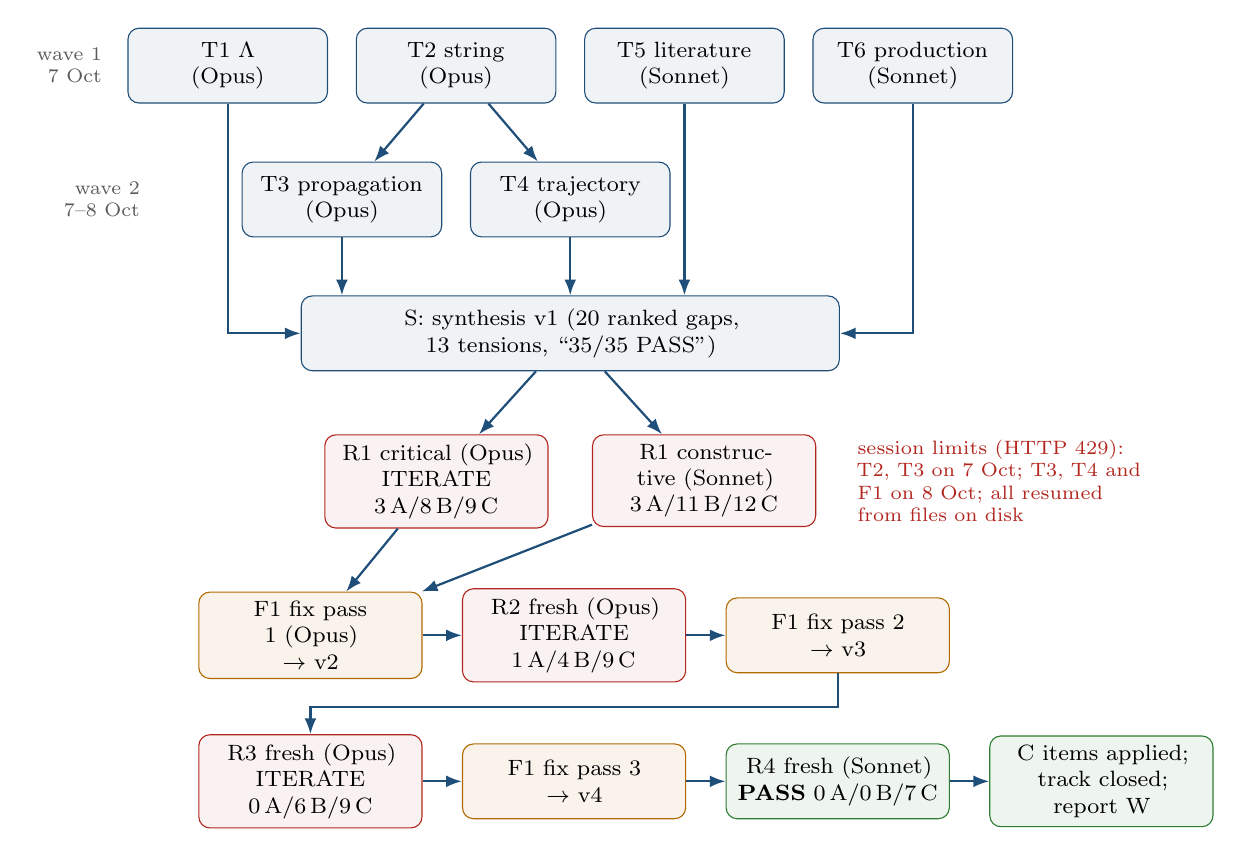
\begin{tikzpicture}[node distance=5mm and 5mm,
  box/.style={draw=acc,fill=acc!7,rounded corners,align=center,minimum height=0.95cm,font=\footnotesize,text width=2.3cm},
  rev/.style={draw=bad,fill=bad!6,rounded corners,align=center,minimum height=0.95cm,font=\footnotesize,text width=2.6cm},
  fix/.style={draw=warn,fill=warn!8,rounded corners,align=center,minimum height=0.95cm,font=\footnotesize,text width=2.6cm},
  arr/.style={-{Latex[length=2mm]},thick,acc}]
\node[box](t1) at (0,0){T1 $\Lambda$\\(Opus)};
\node[box](t2) at (2.9,0){T2 string\\(Opus)};
\node[box](t5) at (5.8,0){T5 literature\\(Sonnet)};
\node[box](t6) at (8.7,0){T6 production\\(Sonnet)};
\node[box](t3) at (1.45,-1.7){T3 propagation\\(Opus)};
\node[box](t4) at (4.35,-1.7){T4 trajectory\\(Opus)};
\node[font=\scriptsize,mid,left=2mm of t1,align=right]{wave 1\\7 Oct};
\node[font=\scriptsize,mid,align=right] at (-1.6,-1.7){wave 2\\7--8 Oct};
\node[box,text width=6.6cm](s) at (4.35,-3.4){S: synthesis v1 (20 ranked gaps, 13 tensions, ``35/35 PASS'')};
\node[rev,below=8mm of s,xshift=-1.7cm](r1c){R1 critical (Opus)\\ITERATE 3\,A/8\,B/9\,C};
\node[rev,below=8mm of s,xshift=1.7cm](r1k){R1 constructive (Sonnet)\\3\,A/11\,B/12\,C};
\node[fix,below=8mm of r1c,xshift=-1.6cm](f1){F1 fix pass 1 (Opus)\\$\to$ v2};
\node[rev,right=of f1](r2){R2 fresh (Opus)\\ITERATE 1\,A/4\,B/9\,C};
\node[fix,right=of r2](f2){F1 fix pass 2\\$\to$ v3};
\node[rev,below=7mm of f1](r3){R3 fresh (Opus)\\ITERATE 0\,A/6\,B/9\,C};
\node[fix,right=of r3](f3){F1 fix pass 3\\$\to$ v4};
\node[rev,right=of f3,draw=ok,fill=ok!8](r4){R4 fresh (Sonnet)\\\textbf{PASS} 0\,A/0\,B/7\,C};
\node[box,right=of r4,text width=2.6cm,draw=ok,fill=ok!8](w){C items applied;\\track closed; report W};
\draw[arr](t1.south)|-(s.west);\draw[arr](t2)--(t3);\draw[arr](t2)--(t4);\draw[arr](t5.south)--(t5.south|-s.north);\draw[arr](t6.south)|-(s.east);
\draw[arr](t3)--(t3.south|-s.north);\draw[arr](t4)--(s);
\draw[arr](s)--(r1c);\draw[arr](s)--(r1k);\draw[arr](r1c)--(f1);\draw[arr](r1k)--(f1);
\draw[arr](f1)--(r2);\draw[arr](r2)--(f2);\draw[arr](f2.south)|-($(r3.north)+(0,0.35)$)--(r3.north);\draw[arr](r3)--(f3);\draw[arr](f3)--(r4);\draw[arr](r4)--(w);
\node[font=\scriptsize,bad,align=left,right=4mm of r1k,text width=3.6cm]{session limits (HTTP 429): T2, T3 on 7~Oct; T3, T4 and F1 on 8~Oct; all resumed from files on disk};
\end{tikzpicture}
\caption{Workflow of the theory track (from \file{LOG.md}). T2 supplied the vacuum propagator to T3 and T4. Each reviewer after R1 was fresh (had not seen the work before). The model of the synthesis agent S is not recorded in the log.}\label{fig:workflow}
\end{figure}

\subsection{Workstreams}
{\small
\begin{longtable}{@{}L{0.8cm}L{5.3cm}L{1.3cm}L{8.4cm}@{}}
\caption{Investigator workstreams \src{README, LOG}.}\label{tab:ws}\\
\toprule ID & Topic & Model & Main output and code\\\midrule\endfirsthead
\toprule ID & Topic & Model & Main output and code\\\midrule\endhead
\bottomrule\endfoot
T1 & $\Lambda$: origin, priors, UV completions, cosmological/astrophysical/collider bounds & Opus & lattice conversion table; GUT ladder strips; freeze-in $T_{\rm RH}$ bound; \file{T1_*.py}, \file{figures/T1_lambda_plane.png}\\
T2 & Vacuum string dynamics: oscillation length, angular momentum, beyond the straight string, semiclassics & Opus & exact closed forms; DY distributions; Athena code review and Python port; 33/33 unit tests; \file{T2_*.py}\\
T3 & Propagation in B and matter: MS, precession, net-charged pairs, timing, stopping, dE/dx & Opus & \file{T3_causal.py} (numba causal string with B + material); 7/7 validation; \file{figures/T3_*.png}\\
T4 & Trajectory model for reconstruction; observables; measuring $(\mQ,\Lambda)$ & Opus & 9-parameter model, degeneracy theorem, Cram\'er--Rao, MET alignment, seeding; \file{T4_*.py}\\
T5 & Literature gap sweep: assumption audit of every quirk paper & Sonnet & 484-record INSPIRE census, 33 papers audited; \file{T5_census.py}, \file{T5_estimates.py}\\
T6 & Production and model space: $\gamma\gamma$, doublets, charges, spin, stopped-pair annihilation & Sonnet & production table, coverage map; \file{T6_*.py}\\
S & Synthesis (v1) & -- & 20 ranked gaps, 13 tensions, spot checks; \file{S_*.py}\\
F1 & Fix passes (v2, v3, v4) & Opus & \file{F1_*.py}: stand-in test, Li phase drift, resolution smearing, stopped-pair reach\\
R1--R4 & Reviewers (R1 critical Opus, R1 constructive Sonnet, R2 Opus, R3 Opus, R4 Sonnet) & & \file{R1_*.py} (independent NG solver, literal Li, Li+MS, B linearity), \file{R2_li_checks.py}, \file{R3_lit_numbers.py}\\
\end{longtable}
}

\subsection{Rules that shaped the result}
\begin{itemize}
\item \textbf{File ownership.} Each agent wrote only its own files (\file{investigations/<ID>_*.md}, \file{code/<ID>_*.py}, \file{figures/<ID>_*}) and appended to \file{LOG.md}. \textbf{No file outside \file{theory_track/} was edited}: the recommended changes to the strategy, signal model, open questions and sample plan are listed in synthesis \S4 (and Section~\ref{sec:mods} here) for the user to apply.
\item \textbf{Evidence tags.} Every number carries a source with location; own calculations are \EST{} with the script named; recalled or secondary numbers are \UNV{}. Killed ideas are reported with the number that kills them.
\item \textbf{Incremental saving.} Agents wrote report skeletons early and appended sections. This mattered: the session limit (HTTP 429) interrupted the work three times (T2 and T3 late on 7~Oct; T3 and T4 on 8~Oct, reset 09:10; F1 during fix pass 1, reset 14:10). Each agent was resumed from its files on disk with no loss \src{LOG}.
\item \textbf{Independence of review.} R1-critical wrote its own Nambu--Goto solver and a literal implementation of the published Li et al.\ algorithm, sharing no propagation code with T2--T4 except the analytic vacuum reference and the object under test. That is what exposed the v1 error (Section~\ref{sec:review}).
\end{itemize}

% ======================================================================
\section{Physics background in brief}\label{sec:physics}
\subsection{Quirks and the benchmark}
A quirk is a heavy particle charged under a new confining gauge group SU($\NIC$) (``infracolour'') that has \emph{no} light infracoloured matter, so the confining flux tube between a quirk and an antiquirk never breaks \cite{KL}. If the confinement scale is far below the quirk mass, the pair produced at the LHC stays bound by a macroscopic string of tension $\sigma$ and oscillates. Throughout, $\Lambda\equiv\sqs$ (the collider convention) and
\begin{equation}
\sigma=50.68\,\frac{\rm GeV}{\rm cm}\left(\frac{\Lambda}{\rm keV}\right)^2 .
\end{equation}
The benchmark is $E=(1,1)_{-1}$, a vector-like Dirac fermion that is a colour singlet with electric charge $\pm1$, with $\NIC=2$, produced by Drell--Yan. The CMS trigger is the MET from an ISR jet recoiling against the pair (the quirks themselves deposit little calorimeter energy), so the triggered sample has $\pTQQ\gtrsim200\GeV$.

\subsection{Oscillation length and number of oscillations}
In the pair rest frame a point-produced pair is an exact one-dimensional ``yo-yo''. With $\gst$ the Lorentz factor of each quirk in that frame at production \src{T2 \S2.1--2.2}:
\begin{align}
\lmax&=\frac{2(\gst-1)\mQ}{\sigma}=3.947\,{\rm cm}\,(\gst-1)\frac{\mQ}{100\GeV}\left(\frac{\keV}{\Lambda}\right)^2,\\
N_{\rm osc}(r<R)&=\frac{\sigma R}{2\beta^*p_T}\approx12\left(\frac{\Lambda}{\keV}\right)^2\quad\text{(CMS tracker, $R\approx1.1$\,m)} .
\end{align}
The natural length is $\ell_0=\mQ/\sigma$. $N_{\rm osc}$ does not depend on $\mQ$. In the lab the vacuum string is straight with a fixed direction, and all propagators agree in vacuum to $\le2\times10^{-8}\,\lmax$ \src{T2 \S2.1}. Everything that distinguishes the methods below happens at first order in the external forces (magnetic field, material), which is exactly the order of the plane thickness.

\subsection{Three ways to propagate the string}\label{sec:methods}
\begin{figure}[H]\centering
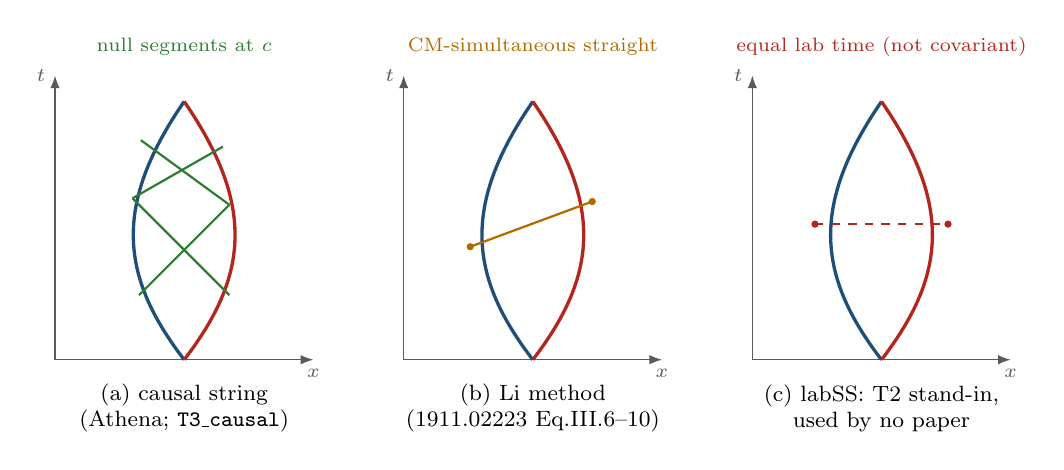
\begin{tikzpicture}[scale=0.82,
  wl/.style={very thick,acc},
  ax/.style={-{Latex[length=1.6mm]},mid}]
% panel a: causal
\begin{scope}
\draw[ax](0,0)--(4.0,0) node[below,font=\scriptsize]{$x$};\draw[ax](0,0)--(0,4.4) node[left,font=\scriptsize]{$t$};
\draw[wl](2,0) .. controls (1.0,1.3) and (0.9,2.4) .. (2,4.0);
\draw[wl,bad] (2,0) .. controls (3.0,1.3) and (3.1,2.4) .. (2,4.0);
\draw[ok,thick] (1.30,1.0)--(2.70,2.40);\draw[ok,thick] (2.70,2.40)--(1.33,3.40);
\draw[ok,thick] (2.70,1.0)--(1.20,2.50);\draw[ok,thick] (1.20,2.50)--(2.60,3.30);
\node[font=\footnotesize,align=center] at (2,-0.75){(a) causal string\\(Athena; \texttt{T3\_causal})};
\node[font=\scriptsize,ok,align=center] at (2.0,4.85){null segments at $c$};
\end{scope}
% panel b: Li
\begin{scope}[xshift=5.4cm]
\draw[ax](0,0)--(4.0,0) node[below,font=\scriptsize]{$x$};\draw[ax](0,0)--(0,4.4) node[left,font=\scriptsize]{$t$};
\draw[wl](2,0) .. controls (1.0,1.3) and (0.9,2.4) .. (2,4.0);
\draw[wl,bad] (2,0) .. controls (3.0,1.3) and (3.1,2.4) .. (2,4.0);
\draw[warn,thick] (1.03,1.75)--(2.92,2.45);
\fill[warn](1.03,1.75) circle (1.6pt);\fill[warn](2.92,2.45) circle (1.6pt);
\node[font=\scriptsize,warn,align=center] at (2.0,4.85){CM-simultaneous straight};
\node[font=\footnotesize,align=center] at (2,-0.75){(b) Li method\\(1911.02223 Eq.III.6--10)};
\end{scope}
% panel c: labSS
\begin{scope}[xshift=10.8cm]
\draw[ax](0,0)--(4.0,0) node[below,font=\scriptsize]{$x$};\draw[ax](0,0)--(0,4.4) node[left,font=\scriptsize]{$t$};
\draw[wl](2,0) .. controls (1.0,1.3) and (0.9,2.4) .. (2,4.0);
\draw[wl,bad] (2,0) .. controls (3.0,1.3) and (3.1,2.4) .. (2,4.0);
\draw[bad,thick,dashed] (0.97,2.1)--(3.03,2.1);
\fill[bad](0.97,2.1) circle (1.6pt);\fill[bad](3.03,2.1) circle (1.6pt);
\node[font=\scriptsize,bad,align=center] at (2.0,4.85){equal lab time (not covariant)};
\node[font=\footnotesize,align=center] at (2,-0.75){(c) labSS: T2 stand-in,\\used by no paper};
\end{scope}
\end{tikzpicture}
\caption{Schematic space-time diagrams (one spatial direction) of the three string prescriptions. Blue and red curves: quirk world lines in a frame where the pair moves. (a) The causal string is built from straight null segments that each endpoint emits and absorbs; signals travel along the string at $c$. (b) The Li method connects the quirks by a straight string at points that are simultaneous in the pair CM frame (a Lorentz-invariant condition), advancing them at different lab times. (c) The lab-time-slice string connects the quirks at equal lab time, a frame-dependent choice. Not to scale.}\label{fig:methods}
\end{figure}

\begin{description}[leftmargin=0.4cm,style=nextline]
\item[Causal string] The Nambu--Goto (NG) string with massive point endpoints, built from straight null segments propagating at $c$; field kicks act on the endpoints. It is an Artru/Lund-type piecewise-null construction. Implementations: the ATLAS Athena \file{Simulation/G4Extensions/Quirks} package (used by FASER), T2's Python port (\texttt{CausalNullString}) and the numba port \file{T3_causal.py}. \textbf{Status: exact classical NG for point masses} (\VER{}, independent conformal-gauge solver, R1). Its validity limit is the NG effective theory itself at near-miss crossings with separation below $1/\Lambda$ (only relevant for $\Lambda\gtrsim10$--$20\keV$) \src{X-13}.
\item[Li method] The Kang--Luty endpoint force with a \emph{straight} string; the quirks are advanced at different lab times so that they stay simultaneous in the pair CM frame, and the string direction is built from the separation and the quirk velocity [1911.02223 Eq.III.6--10 = 2002.07503 Eq.VIII.1--4]. Covariant by construction; neglects string curvature and retardation. Used by Li et al.\ \cite{LiLi,traj}; the other published central-detector studies \cite{Knapen,Sha} also use straight-string integrators, but their exact prescription and step are not known.
\item[labSS] A straight string between the two quirks at equal \emph{lab} time. T2 and T3 wrote it as a stand-in for the Li method. \textbf{No published paper uses it}; it is not Lorentz covariant. (cmSS, a second T2 variant that approximates CM simultaneity by linear extrapolation, is not in the literature either.)
\end{description}

\subsection{Observables and the meaning of ``truth level''}
\begin{itemize}
\item \textbf{Plane thickness} $\Ds$: the square root of the smallest eigenvalue of $\sum h h^T/(N-1)$ over the hits $h$ of both quirks, for a plane through the primary vertex [1708.02243 Eq.11; 2002.07503 Eq.C.1]. The coplanar search cuts on it (strategy: $\Ds<100\um$).
\item \textbf{Literature formula} $d=1.16\um\,(\mQ/100\GeV)(\keV/\Lambda)^4(B/{\rm T})$ [1911.02223 Eq.III.12]: a first-order perturbative estimate; it describes the odd-crossing miss distance, not the accumulated plane-fit thickness \src{X-2}.
\item \textbf{Truth level}: true hit positions, no detector resolution, known hit-to-quirk assignment, no pile-up. All thickness efficiencies in the investigator reports are truth level. $t_{\rm est}$ is the thickness estimated from \emph{smeared} hits with a resolution-weighted plane fit \src{S-2}.
\item \textbf{Regimes in $\Lambda$.} $\Lambda\lesssim0.3\keV$: less than one oscillation in the tracker for $\approx45\%$ of triggered pairs; 0.45--20\,keV: the coplanar oscillating-pair regime; $\gtrsim20$--$30\keV$: the pair is merged into one highly ionising object; $\gtrsim3\MeV$: prompt annihilation into a resonance at $2\mQ$ \src{Box A; T6}.
\end{itemize}

% ======================================================================
\section{Discoveries and results}\label{sec:results}
This section follows the user's four topics, then the other gaps, then the ranked list. Numbers are synthesis v4 values with their tags; ``truth level'' is stated wherever it applies.

\subsection{The confinement scale \texorpdfstring{$\Lambda$}{Lambda}}\label{sec:lambda}
{\small
\begin{longtable}{@{}L{3.0cm}L{10.4cm}L{3.0cm}@{}}
\caption{What is known about $\Lambda$ after this track (synthesis Box~A, consolidated).}\label{tab:boxA}\\
\toprule Question & Answer & Source / status\\\midrule\endfirsthead
\toprule Question & Answer & Source / status\\\midrule\endhead
\bottomrule\endfoot
Convention & $\Lambda\equiv\sqs$. Lattice SU(2)/SU(3): $T_c/\sqs=0.709/0.646$, $\Lambda_{\overline{\rm MS}}/\sqs=0.581/0.542$, $m_{0^{++}}/\sqs=3.78/3.41$. The cosmology paper's ``$\Lambda$'' is $T_c$, so its 1\,keV is $\sqs=1.41\keV$ (SU(2)); our \file{theory_signal_model.md}'s $1/0.6$ is 18\% off. A 1-loop ``$\Lambda$'' read as $\sqs$ is off by $\times8$. For non-fundamental representations or $\NIC\ge4$, $\sigma_k/\sigma_1$ follows Casimir or sine-law scaling (\UNV{}), so $\Lambda$ must be defined per representation & T1 G-T1-1; S check 5 (\VER{}); S-11\\
Existing exclusions ($E$ singlet, $\NIC=2$) & \textbf{Farina--Low} recast of CMS HSCP + monojet (12.9\fbinv): $\mQ>650\GeV$ at $\Lambda=1$\,eV, $>150\GeV$ at 100\,eV, none at 1\,keV [1703.00912 Tab.II] (scalar 350/60\,GeV). \textbf{Evans--Luty} recast of the CMS out-of-time search (38.6\fbinv): $\lesssim0.1\TeV$, only at $\Lambda\lesssim0.15\keV$. \textbf{D0}: 107\,GeV for 10\,keV--1\,MeV. \textbf{FASER} (186\fbinv; HEPData ins3184325 t2, as quoted in \file{theory_signal_model.md} \S6.3): 57/72/113/149/163/179/173\,GeV at $\Lambda$ = 0.3/0.5/1/1.7/3/10/30\,keV and 71\,GeV at 100\,keV. No tabulated point at 20 or 50\,keV (v4's by-eye readings: $\approx175$/155\,GeV, \UNV{}). Synthesis v4 used by-eye readings throughout, 8--14\,GeV lower at 1--3\,keV (Section~\ref{sec:owndisc}). Nothing above $\approx0.18\TeV$ in 0.3--100\,keV & 1703.00912; 1811.08903 Fig.5; 1008.3547; 2607.26195 + HEPData\\
Where the tracker is sensitive & 50\% edge of the $\Ds<100\um$ finder at $\Lambda_{\rm low}\approx0.5/0.45/0.55\to0.7\keV$ (200/500/1000\,GeV; B $\to$ B+material) at \textbf{truth level}; $\ge90\%$ from $\approx1\keV$ (200--500\,GeV) or $\approx2\keV$ (1\,TeV); upper edge from pair merging at $\approx20$--30\,keV. With realistic resolution the lower edge is undefined until a cut is set at fixed background efficiency & T3 \S9; S-2, S-3\\
Below / above the window & $\Lambda<0.3\keV$ ($<1$ oscillation for 44--47\% of triggered pairs at 0.3\,keV) and $\Lambda\gtrsim30\keV$: only stopped-pair (S-8) and merged-pair (S-10) channels. $\Lambda\gtrsim3\MeV$: prompt annihilation; dilepton/diphoton resonances probably exclude $\mQ\lesssim0.8$--1\,TeV (\UNV{}). 0.1--3\,MeV: displaced annihilation, no search (S-16) & T2 \S3; T6 G-T6-5\\
Theory prior & SUSY-GUT ladder [0805.4642 Sec.2.5]: SU(2), $n_S=3$: $\sqs\approx0.8/2.6/6.4/15\keV$ at 0.2/0.5/1/2\,TeV ($\times/\div3.9$). Its EW quirks are \emph{doublets}, which decay to the neutral member ($c\tau=7.8$\,mm) before the first pixel layer. Neutral naturalness predicts GeV, not keV. The $E$ coplanar search is motivated by generic hidden sectors (log-flat prior: $\approx6\%$ of a $\times2$ prior in $\alpha^{-1}$ lands in the window) & T1 G-T1-2, -3, -6\\
Cosmology & If the IC sector ever thermalised, the whole window is excluded ($\Omega_Gh^2\approx2$--$10\,(\sqs/\keV)$). A discovery implies UV freeze-in with $T_{\max}\lesssim\mQ/25$ and $T_{\rm RH}\lesssim5$--40\,GeV (0.2--1\,TeV). Glueballs are stable ($\tau\ge10^{35}$\,s); no BBN/CMB decay bound & T1 G-T1-4; S-15\\
Measuring $\Lambda$ & Hits measure only $\ell_0=\mQ/\sigma$. With the MET recoil: $\sigma(\Lambda)/\Lambda\approx0.5\%$ (statistical, 30 events), 0.5--1.5\% with the MET scale. B-only route for $\Lambda\lesssim2\keV$ & T4 \S4; S-4\\
$\NIC=3$ & rate $\times1.5$; $T_c/\sqs=0.646$; $\Delta N_{\rm eff}$ (thermal) 0.57 instead of 0.21 & T1; S-11\\
\end{longtable}
}

\begin{figure}[p]\centering
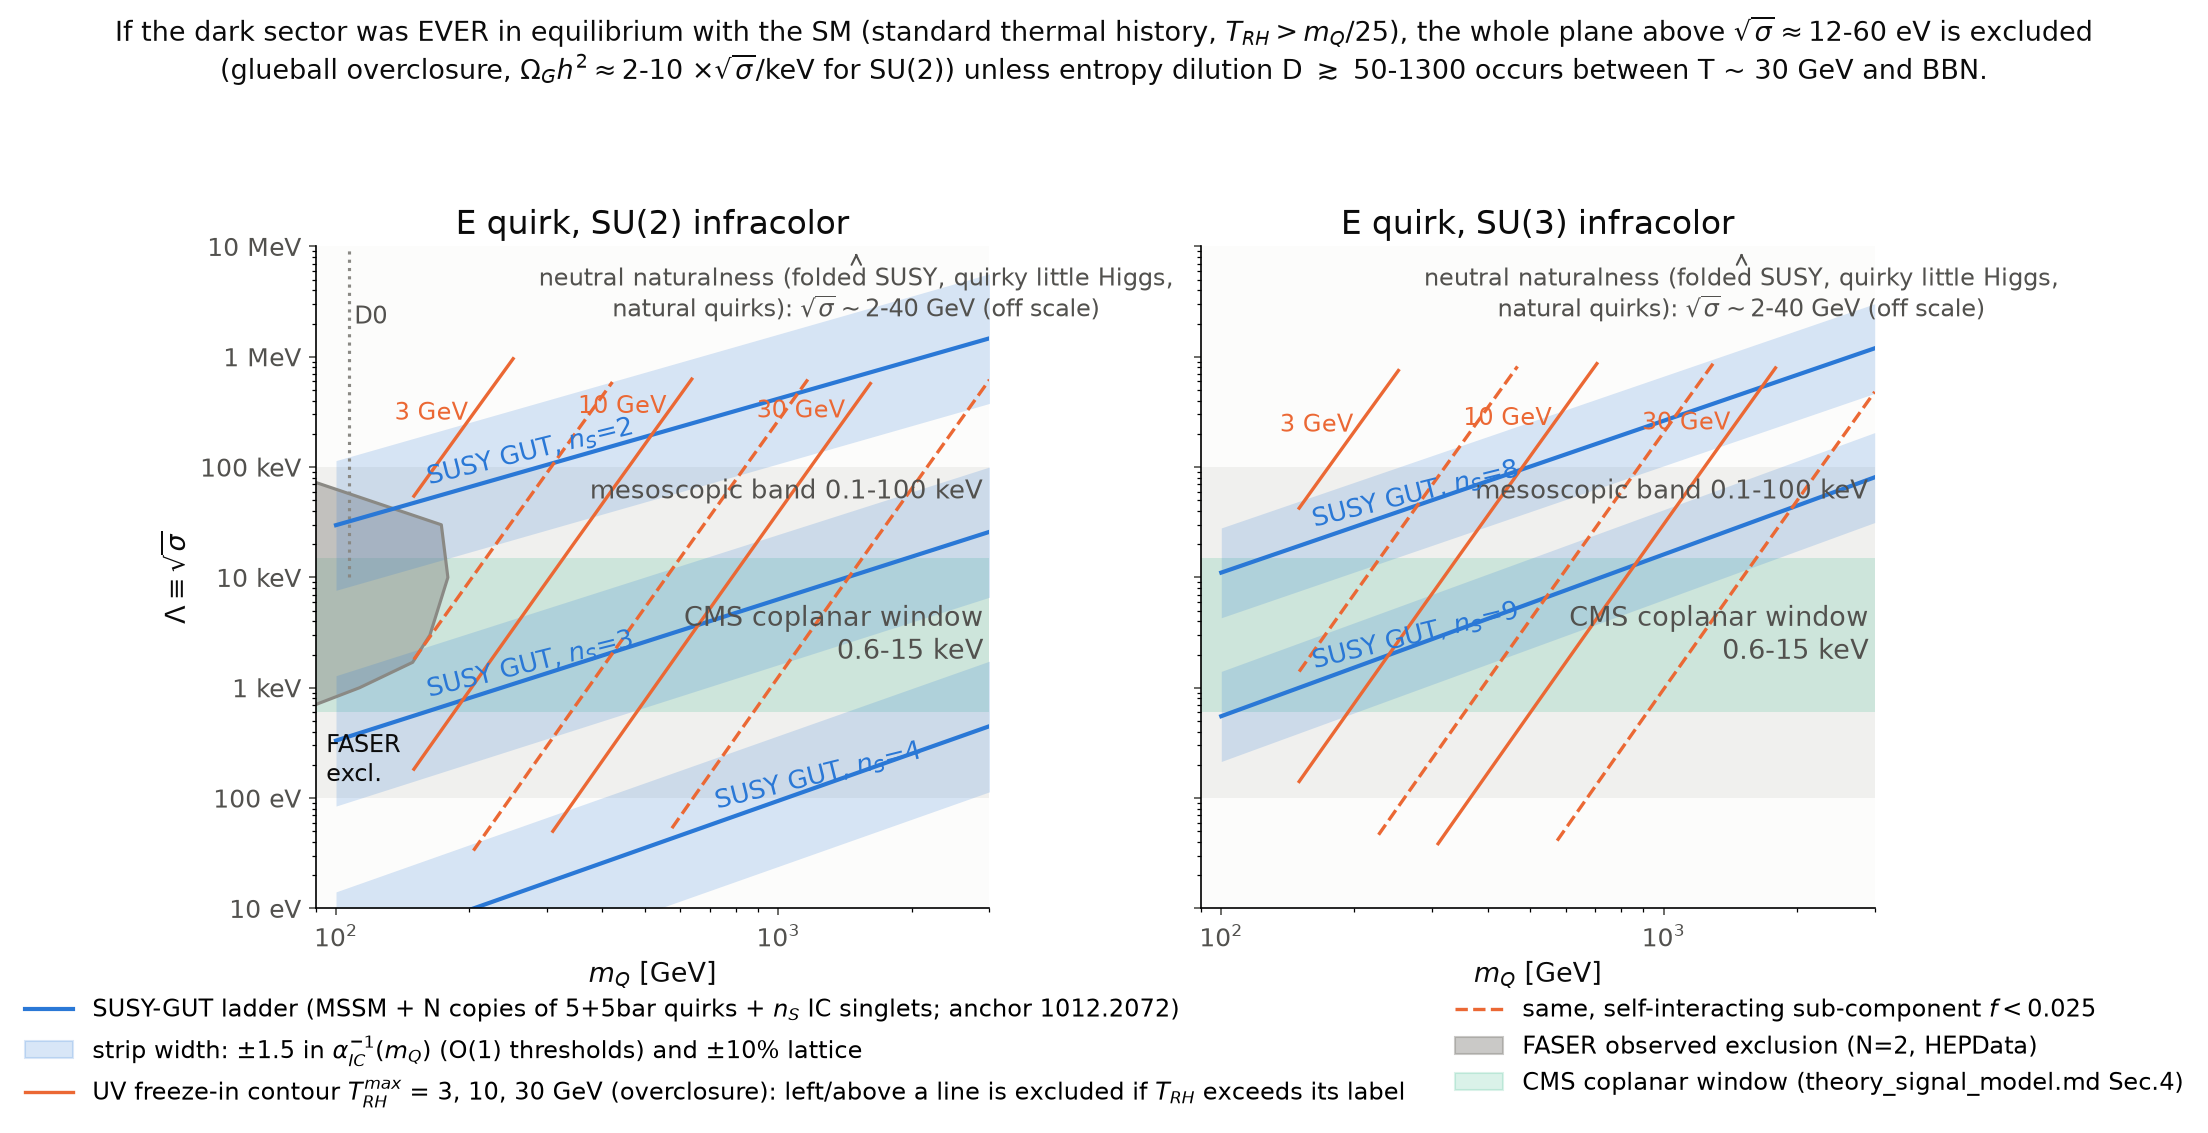
\includegraphics[angle=90,height=0.74\textheight]{figures/T1_lambda_plane_rep.png}
\caption{\textbf{T1 overview of the $(\mQ,\Lambda)$ plane} for the $E$ quirk, SU(2) (left) and SU(3) (right) \src{T1; \file{code/T1_figure.py}; \EST{}}. Blue: SUSY-GUT ladder strips ($\pm1.5$ in $\alpha_{\rm IC}^{-1}$ and $\pm10\%$ lattice); \emph{these strips are motivated by doublet quirks, not by $E$} (S-14), so they are a motivation overlay only. Orange: UV freeze-in contours of the maximal reheat temperature (overclosure, solid; self-interacting sub-component, dashed). Grey: FASER (HEPData) and D0. Green band: the \emph{pre-track} CMS coplanar window 0.6--15\,keV from \file{theory_signal_model.md} \S4; the truth-level lower edge from this track is 0.45--0.7\,keV (Table~\ref{tab:boxA}). The freeze-in contours carry T1's normalisation, which is $\times2.2$ above 2512.20696 Fig.~4 in $T_{\rm RH}$ (unresolved, Section~\ref{sec:disc}). Fonts enlarged for this report (\file{report/figures/regen_report_figures.py}); content unchanged.}\label{fig:T1}
\end{figure}

\subsection{Oscillation length}\label{sec:osc}
\begin{itemize}
\item \textbf{Exact closed forms} \src{T2 \S2.1--2.2; S check 1, \VER{}}: $\lmax=3.947\,{\rm cm}\,(\gst-1)(\mQ/100\GeV)(\keV/\Lambda)^2$; full CM period $T^*=4p^*/\sigma$; $N_{\rm osc}=\sigma R/(2\beta^*p_T)\approx12(\Lambda/\keV)^2$ in the CMS tracker, independent of $\mQ$; about $24(\Lambda/\keV)^2$ crossings. (Li et al.\ computed the number of periods numerically [2002.07503 \S IV]; this is a closed form of the same quantity.) Li's lab closed form [2002.07503 Eq.II.4--8] is exact in vacuum.
\item \textbf{Typical values} (triggered, medians): $\lmax=5.4$\,cm (500\,GeV, 1\,keV), 0.54\,mm (10\,keV), 60\,cm (0.3\,keV) \src{T2 Tab.3.1}.
\item \textbf{Literature shorthands}: ``2\,cm$(\gamma-1)$'' is a factor 2 too small (systematic). ``1\,cm $\times(m/100\GeV)$ $\times(\keV/\Lambda)^2$'' [2404.13814; 2607.26195; 2512.20696] is right on average for $E$ near 500\,GeV but wrong by $\times0.4$--2.7 event by event (Figure~\ref{fig:osc}, top left).
\item \textbf{Scalars $\tilde E$} (P-wave production): $\lmax\times1.70$--1.73 (median) and $N_{\rm osc}\times0.81$ \src{T2 \S3}. The scalar alternate needs its own window.
\item \textbf{ISR modelling}: a fixed-$p_T$ ISR kick biases $\lmax$ by $-10$ to $-25\%$ and $N_{\rm osc}$ by $+20\%$; generate with a $V$+jet matrix element \src{S-13}.
\end{itemize}

\begin{figure}[!htbp]\centering
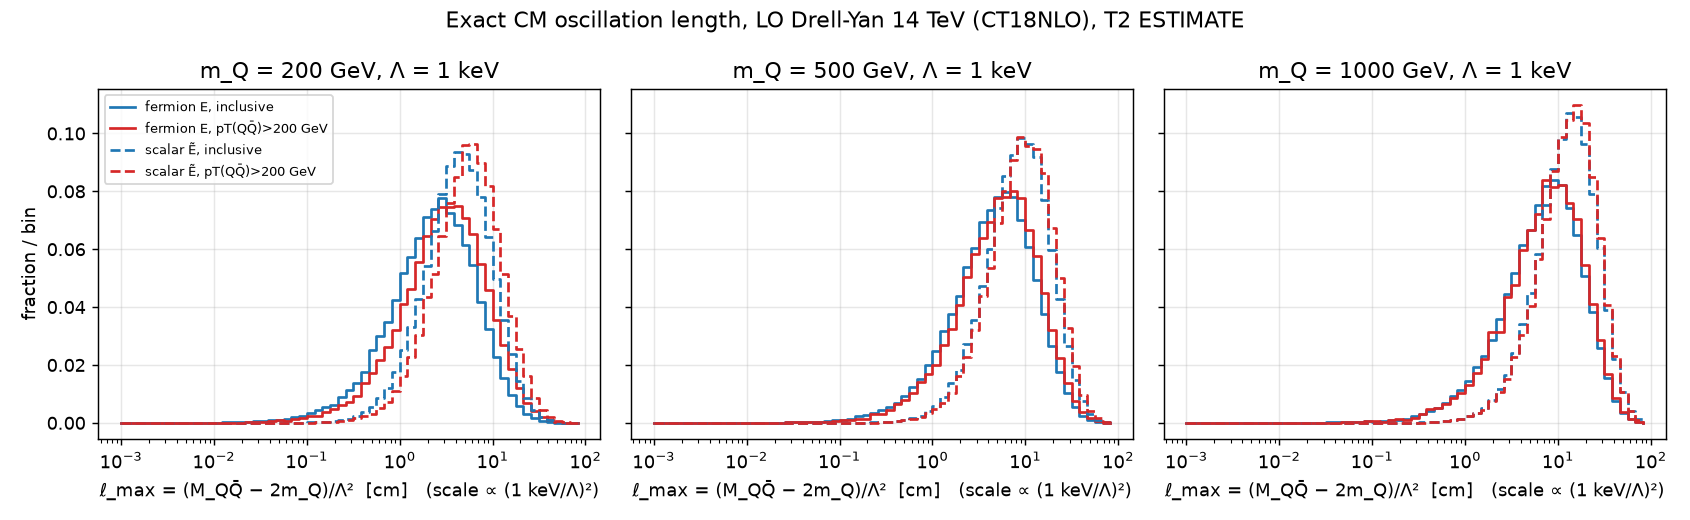
\includegraphics[width=\textwidth]{figures/T2_lmax_distributions.png}\\[2pt]
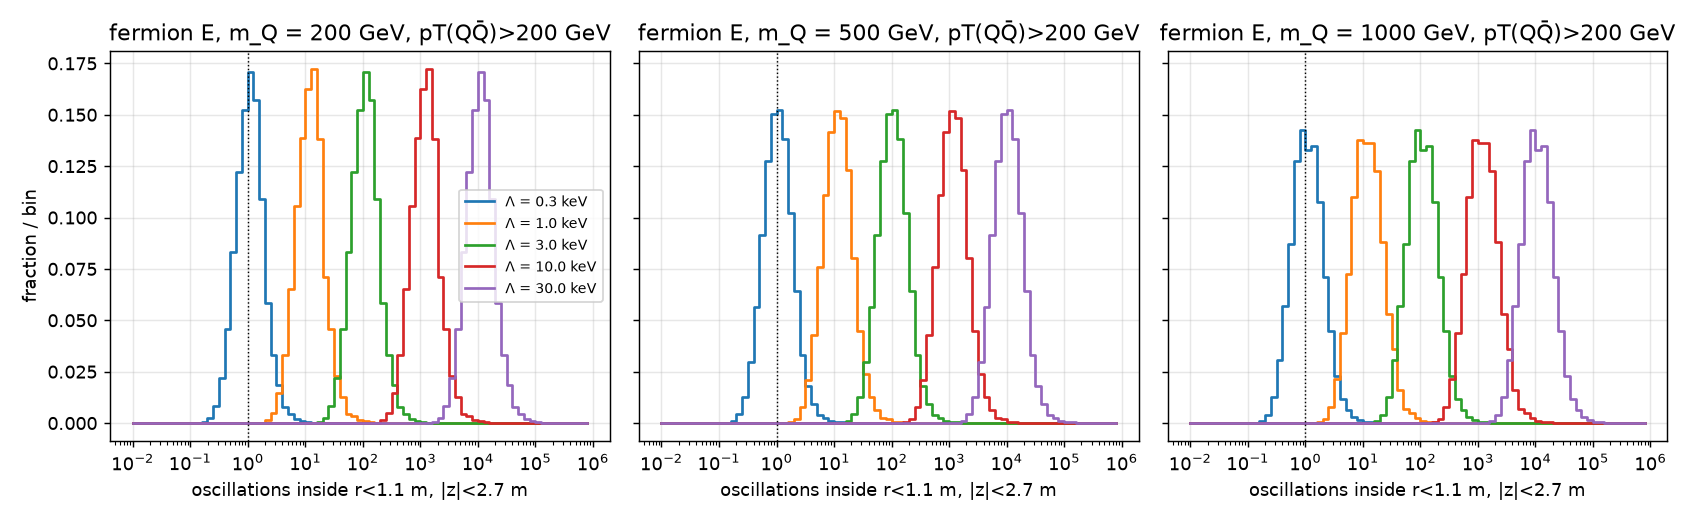
\includegraphics[width=\textwidth]{figures/T2_nosc_tracker.png}
\caption{\textbf{Oscillation length and number of oscillations} for LO Drell--Yan $E$ pairs at 14\,TeV \src{T2 \S3; \file{code/T2_kinematics.py}; \EST{}; not affected by the T2 erratum}. Top: exact CM $\lmax$ at $\Lambda=1\keV$ (scales as $(1\keV/\Lambda)^2$), fermion and scalar, inclusive and with $\pTQQ>200\GeV$. Bottom: oscillations inside the CMS tracker ($r<1.1$\,m, $|z|<2.7$\,m) for $\Lambda=0.3$--30\,keV; the distributions are the same for all three masses ($N_{\rm osc}$ is $\mQ$-independent).}\label{fig:osc1}
\end{figure}

\begin{figure}[!htbp]\centering
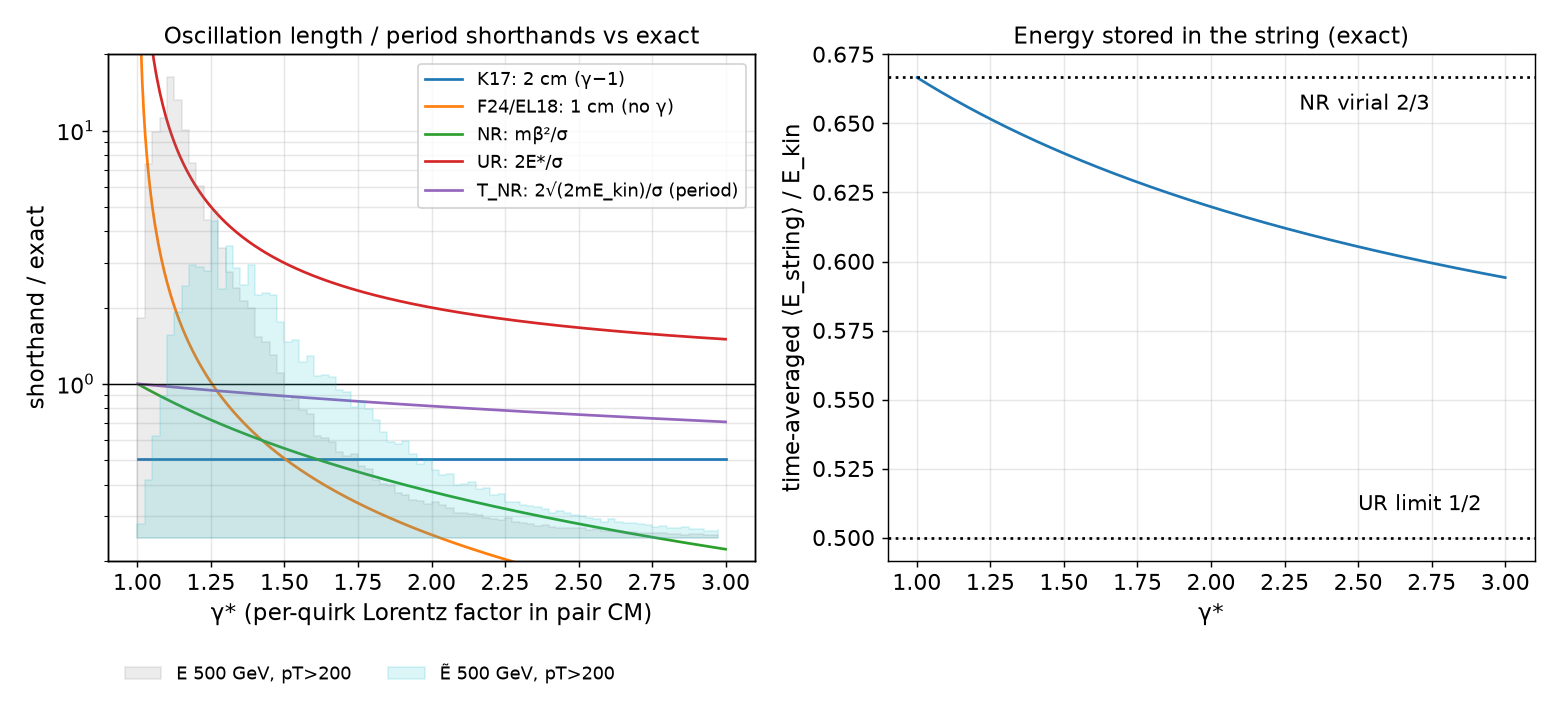
\includegraphics[width=0.95\textwidth]{figures/T2_approx_errors_rep.png}\\[2pt]
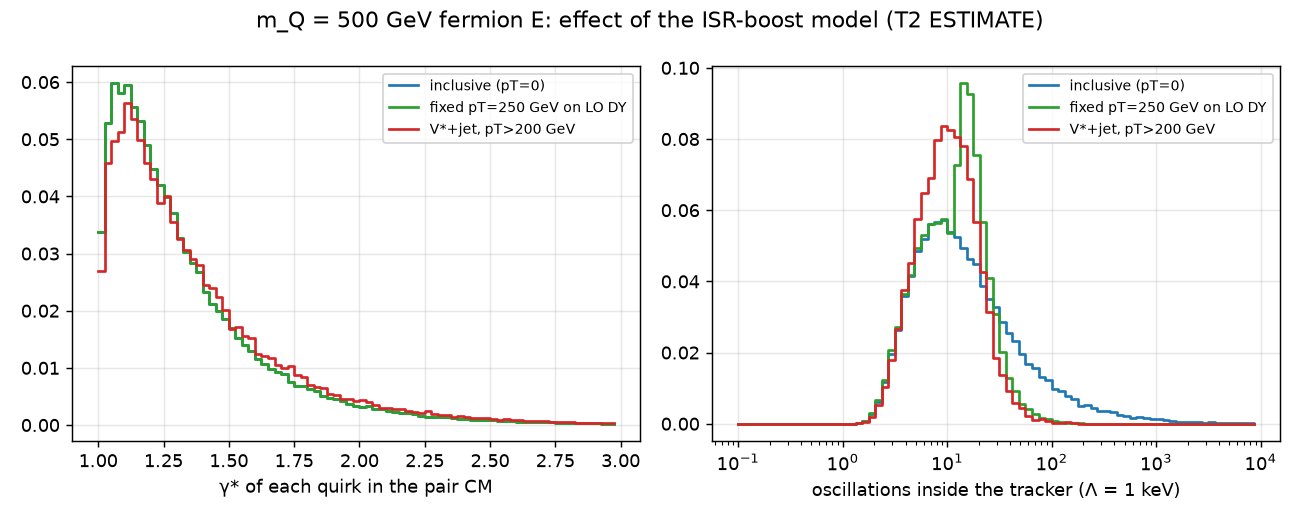
\includegraphics[width=0.85\textwidth]{figures/T2_isr_assumptions.png}
\caption{\textbf{Accuracy of the literature shorthands and of ISR modelling} \src{T2 \S2.4, \S3; \file{code/T2_approx_errors.py}, \file{code/T2_kinematics.py}; \EST{}, vacuum only, unaffected by the erratum}. Top left: ratio of shorthand to exact $\lmax$ (or period) vs $\gst$, with the triggered $\gst$ distributions for $E$ and $\tilde E$ at 500\,GeV underlaid; top right: time-averaged string energy fraction. Bottom: $\gst$ and $N_{\rm osc}$ (1\,keV) for inclusive pairs, a fixed $p_T=250\GeV$ kick, and a $V^*$+jet matrix element with $p_T>200\GeV$; both bottom y-axes are the fraction per bin. Top figure re-drawn with larger fonts (legends moved, annotation no longer overlapping).}\label{fig:osc}
\end{figure}

\subsection{Propagation dynamics}\label{sec:prop}
\subsubsection{The trajectory model: causal string validated; Li method $\gst$-dependent; lab slices unusable \src{S-1}}
\textbf{Context.} The question was posed but never tested in the literature: Kang and Luty asserted that the CM string stays straight and that ``it would be useful to check this by direct simulation'' [0805.4642 \S3.2]; Evans--Luty wrote that ``retarded time corrections can also be safely neglected'' [1811.08903 \S2]. S-1 is that check. Table~\ref{tab:S1} gives the evidence (all at $\mQ=500\GeV$, 3.8\,T, no material unless stated, 10 barrel radii).

{\small
\begin{longtable}{@{}L{4.1cm}L{9.0cm}L{3.3cm}@{}}
\caption{Evidence behind S-1 (synthesis v4 S-1 table).}\label{tab:S1}\\
\toprule Comparison & Result & Source\\\midrule\endfirsthead
\toprule Comparison & Result & Source\\\midrule\endhead
\bottomrule\endfoot
Causal port vs \textbf{independent conformal-gauge NG solver} & thickness ratio \textbf{0.990--1.004}; out-of-plane hit differences $\le0.4\um$; all hits $\le8.2\um$ (16 events, 0.6--3\,keV); canonical momentum conserved to $\le2\times10^{-3}\GeV$ & R1 \file{R1_conformal_ng.py} (\VER{}, indep.)\\
Literal Li integrator, step-converged, vs causal ($\gst=1.28$, $p_T=300\GeV$) & thickness ratio 0.84--1.04, median $\approx0.85$ (0.6--2\,keV, 18 events); max OT-hit difference 53--80\um\ (0.6\,keV), 27--430\um\ (1\,keV) & R1 \file{R1_li_literal.py} (\VER{})\\
Same, on T2's own events (the events behind the v1 numbers) & Li/causal 0.84--1.05 (median 0.88); labSS/causal 1.5--75 (median 8.9); \textbf{labSS/Li = 1.6--73, 0 of 12 events within $\pm50\%$} & F1 \file{F1_standin.py}\\
Li at its \textbf{printed step bound} [1911.02223 Eq.III.10] & thickness $\times0.8$--20 off (0.6--3\,keV; $\times10$--70 at 5\,keV), OT hits 6--250\,mm off: Euler non-convergence. The step Li et al.\ actually used is unknown & R1; F1\\
Convergence vs $\Lambda$ & Required fraction of the printed bound falls roughly as $\Lambda^{-2}$ (step must resolve near-miss crossings, $b\propto\Lambda^{-4}$); cost $\propto\Lambda^4$: $\sim10^8$ steps/event at 2\,keV. 3\,keV converged at $\times10^{-3}$ (0.855/0.856); 5\,keV untested below $\times10^{-2}$ & R1; R2 \file{R2_li_fine_out.txt}\\
\textbf{$\gst$ dependence} (1\,keV, 5 events per point) & median Li/causal \textbf{0.97 / 0.85 / 0.92 / 0.69 / 0.65 at $\gst$ = 1.05 / 1.28 / 1.6 / 2 / 3}; single events 0.53--1.36 at $\gst\ge2$; out-of-plane differences up to 124\um. At $\gst=3$ all 5 events have different hit counts; matched evidence for 30--35\% is $\gst=2$ (0.68). $\Lambda$-independence tested only at $\gst=1.28$; $\gst$ dependence only at 1\,keV & R2 \file{R2_li_checks.py} (\VER{})\\
Residual mm hit differences at 2\,keV & step non-convergence of Li: max $|\Delta{\rm hit}|$ 0.2--9.8\,mm ($\times0.003$) $\to$ 0.07--0.53\,mm ($\times0.001$); an in-plane phase drift; out-of-plane $\le10.5\um$; no effect on the plane finder & F1 \file{F1_li_phase.py}\\
Li + MS vs causal + MS ($B=0$) & median 13 vs 30\um\ (1\,keV), 11.9 vs 15\um\ (3\,keV); no secular growth, no mm-scale thickness. The ``fake 0.2--21\,mm'' of T3 \S3.1 is a labSS property & R1 \file{R1_li_ms.py}\\
Knapen--Papucci code; Sha et al.\ GNN samples & prescription and step unknown; nobody on the track has seen the code. \textbf{Status unknown} & --\\
\end{longtable}
}

\begin{key}
\textbf{What survives (S-1, rank 1, \EXPL{}, days, confidence high).} (i) The causal string (\file{T3_causal.py}) is exact classical NG with point endpoints and is the production model; its caveat is the NG effective theory at near-miss crossings, negligible for $\Lambda\lesssim3$--10\,keV and a 10--30\% model uncertainty on the B-thickness at $\Lambda\gtrsim10$--20\,keV (\EST{}). (ii) The Li method is good when converged, with a $\gst$-dependent deficit (3\% / 15\% / 30--35\%). (iii) Lab-time-slice straight strings, the naive choice for a fast propagator, are badly wrong ($\times1.5$--75). (iv) Knapen--Papucci and Sha et al.: unknown until inspected. \textbf{No fixed ratio is a valid validation target}: compare event by event in bins of $\gst$ over the triggered spectrum, check step convergence directly, and match crossings by index.
\end{key}

\begin{figure}[!htbp]\centering
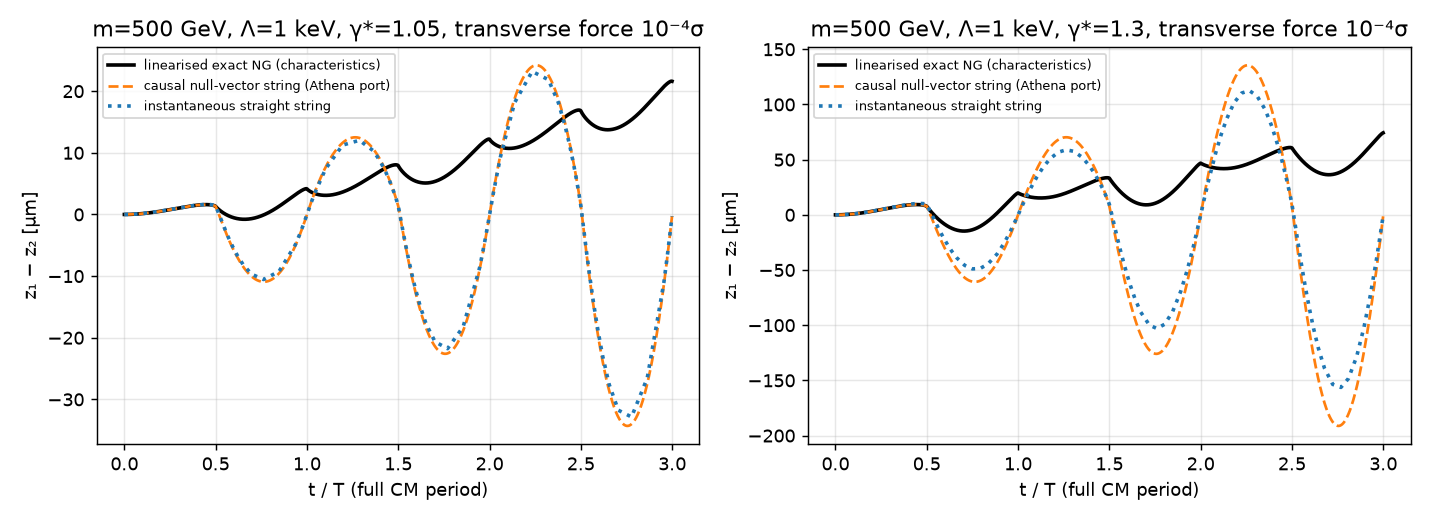
\includegraphics[width=0.95\textwidth]{figures/T2_transverse_check.png}
\caption{\textbf{Causal vs straight string for a pair at rest} in a weak transverse force $10^{-4}\sigma$ ($\mQ=500\GeV$, $\Lambda=1\keV$; left $\gst=1.05$, right $\gst=1.3$) \src{T2 \S5.1 item 3; \file{code/T2_transverse_linear.py}; \EST{}}. Out-of-plane separation $z_1-z_2$ vs time in units of the CM period. The dotted straight string is T2's labSS code, but because the pair is at rest, lab and CM simultaneity coincide, so here it is effectively the CM-simultaneous prescription, not the \WD{} moving-pair labSS case. The linearised NG solution (black) is valid only up to the first crossing ($t/T=0.5$), where all three agree. Causal and straight agree to $\approx3\%$ at $\gst=1.05$ and differ by $\approx20\%$ in amplitude at $\gst=1.3$; this trend is qualitatively the same as R2's $\gst$-dependent Li deficit (the figure itself is not cited in synthesis v4, and no step-convergence test was run for it).}\label{fig:transverse}
\end{figure}

\subsubsection{Plane-thickness physics and the revised window \src{S-3}}
The project's strategy uses $d=1.16\um\,(\mQ/100\GeV)(\keV/\Lambda)^4(B/{\rm T})$ [1911.02223 Eq.III.12] to set the window edge. \textbf{Credit:} Li et al.\ themselves show that their numerical thickness deviates from this formula by $10^{-3}$--$10^{3}$ and agrees only ``within an order of magnitude'' [2002.07503 App.C, Fig.8]; their published reach uses the numerical thickness. So the formula's failure is a criticism of \emph{this project's} use of it, not of published analyses. The causal string gives (B only, truth level, median) \src{T3 \S3.2}:

\begin{center}\small
\begin{tabular}{@{}cccc@{}}\toprule
$\mQ$ [GeV] & $\Lambda$ [keV] & causal B-only $\Ds$ & formula $d$\\\midrule
200--1000 & 1 & 32--38\um & 9--44\um\\
200--1000 & 3 & 3.9--5.2\um & 0.1--0.55\um\\
200--1000 & 10 & 0.4--0.7\um & $\le0.004\um$\\\bottomrule
\end{tabular}\end{center}

\begin{itemize}
\item \textbf{Already in Li et al.}\ [2002.07503 \S V, Fig.4]: the thickness depends only mildly on $m$ and $p_T$; local exponents $\approx\Lambda^{-1.9}$ and $\Lambda^{-1.3}$ (R3's by-eye reading); $\approx\times50$ above the formula at 2\,keV; linear in the quirk charge [\S V.A].
\item \textbf{New here:} (i) local exponents $\Lambda^{-1.6\ldots-2.0}$ (median $\approx-1.9$) and $\sim\mQ$ independence measured with a validated, converged propagator over 1--10\,keV; (ii) T4's in-plane B displacement $x_B\approx0.5\,qBR/\sigma$ shows the same scaling; (iii) \textbf{the response is non-linear in $B$}: exactly linear before the first crossing, then $\approx1+0.10\ln(B_0/B)$ (31--35\% at $B/20$), \VER{} by the independent conformal-gauge solver [R1 \file{R1_Blinearity.py}; S \file{S_Bnonlin.py}, \file{S_Bscan.py}], so Li's ``linear in $q$'' holds only to $\approx10\%$; (iv) the crossing origin of the thickness; (v) the MS floor; (vi) the corrected window.
\item \textbf{Heuristic mechanism} (\EST{}; coefficient fitted, not derived): at a crossing the partner is offset by $b\propto qB$; the string pulls transversely with $\sigma b/|x|$ while $|x|\to0$, so the impulse $\int\sigma b/(v|t|)\,dt$ is cut off at $|x|\sim b$, giving $(\sigma b/v)\ln(\ell/b)$: a $B\ln(1/B)$ term. With $b\propto B/\Lambda^4$ and $\ell\propto1/\Lambda^2$ it predicts $B^{0.89\text{--}0.92}$ and $\Lambda^{-1.78\ldots-1.84}$, matching the measured $B^{0.91}$ and $\Lambda^{-1.6\ldots-2.0}$. The formula $d$ is the odd-crossing miss distance $b\approx3.5\um(\keV/\Lambda)^4$, not the accumulated thickness \src{X-2}.
\item \textbf{Revised window (truth level):} 50\% edge $\Lambda_{\rm low}\approx0.5/0.45/0.55\to0.7\keV$ at 200/500/1000\,GeV, slightly lower and flatter in $\mQ$ than the strategy's 0.54--0.81\,keV; at 1\,TeV the $\ge90\%$ plateau starts at $\approx2\keV$ (MS). Upper edges unchanged. Effect on the projected reach: not computable at our precision.
\end{itemize}

\begin{figure}[!htbp]\centering
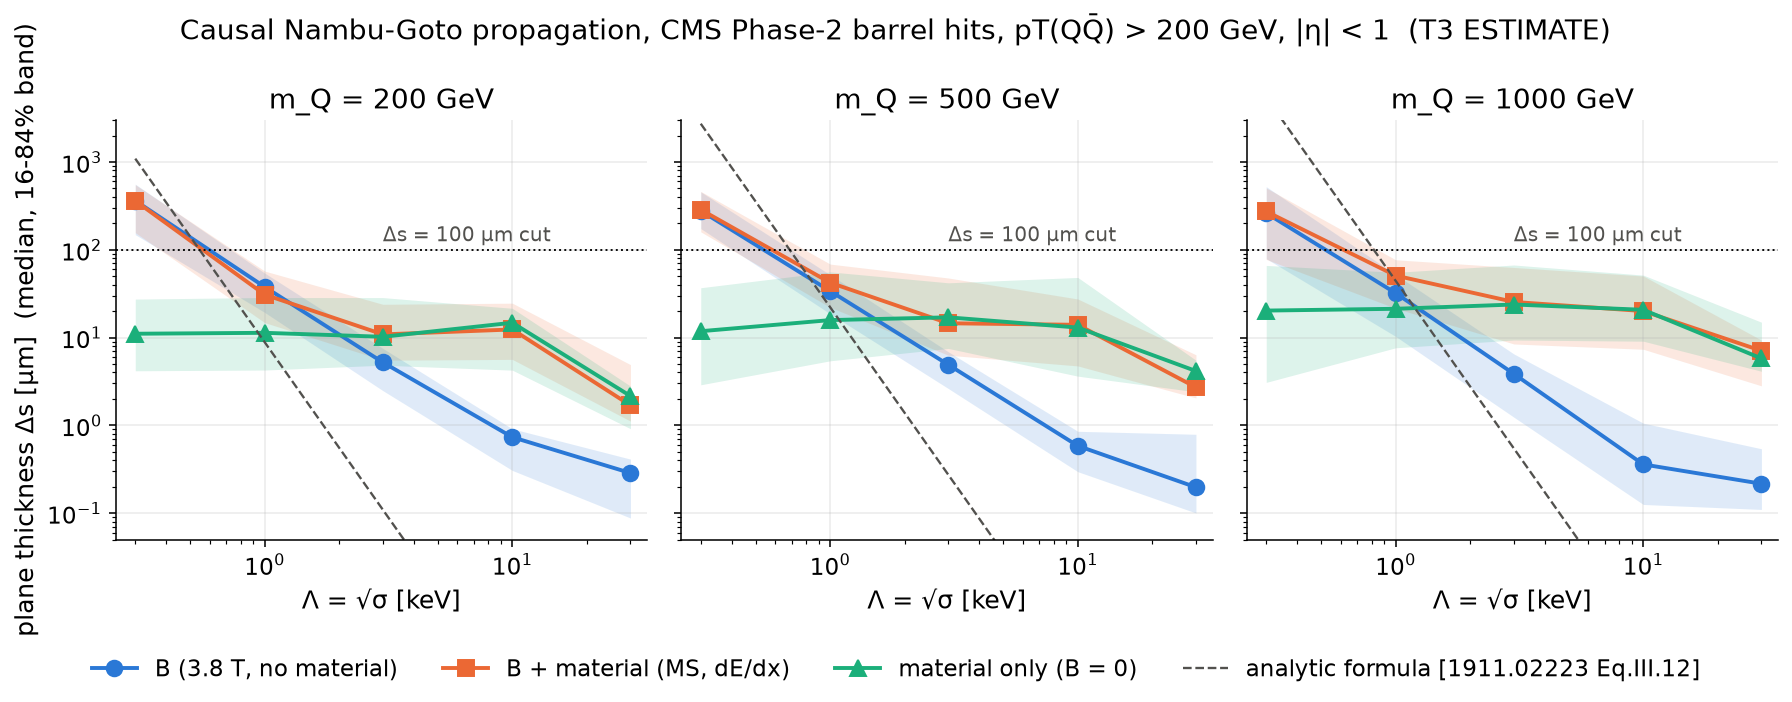
\includegraphics[width=\textwidth]{figures/T3_ms_thickness_rep.png}
\caption{\textbf{Plane thickness vs $\Lambda$ with the causal string} \src{T3 \S3.2; \file{code/T3_ms_thickness.py}, \file{code/T3_ms_figure.py}; \EST{}, truth level}. Median and 16--84\% band for B only (blue), B + Phase-2 material (MS, dE/dx; orange) and material only (green), at $\mQ=200/500/1000\GeV$, $\pTQQ>200\GeV$, $|\eta|<1$; dashed: the analytic formula [1911.02223 Eq.III.12]; dotted: the 100\um\ cut. Legend moved below the panels for this report. Material per layer is \UNV{} ($\approx19\%\,X_0$ at $\eta=0$). This figure uses only the causal string and is not affected by the erratum. Statistics: 60 events per point for $\Lambda\le3\keV$, 24 at 10\,keV, 12 at 30\,keV.}\label{fig:T3ms}
\end{figure}

\subsubsection{Multiple-scattering floor and realistic hit resolution \src{S-2}}
\begin{itemize}
\item \textbf{Credit and novelty.} No published phenomenology study includes MS or quantifies it (Knapen neglect material; Li et al.\ include only the mean dE/dx; Evans--Luty ``have not attempted to model'' the kicks; Sha et al.\ smear hits by 1\,mm). The ATLAS/FASER Athena Geant4 extension uses ``standard Geant4 electromagnetic processes'' [2607.26195 App.A], so it probably includes MS (\UNV{} which processes), but no effect on quirk observables has been published. New here: the quantification for the CMS Phase-2 central detector. T5's earlier 50--400\um\ bound is superseded \src{X-7}.
\item \textbf{Truth-level floor}: median $\Ds_{\rm MS}=11/15/22\um$ at 200/500/1000\,GeV, nearly $\Lambda$-independent (84th percentile $\le67\um$); MS dominates the B thickness for $\Lambda\gtrsim1.5$--2\,keV. Pass fraction of $\Ds<100\um$ (B + material): 0.93--1.00 for 1--30\,keV. A $\Ds<30\um$ cut keeps 0.92--0.93 / 0.68--0.83 / 0.55--0.67 at 3--10\,keV. $\Ds_{\rm MS}\propto(x/X_0)^{0.517}$ (a scaling of the same code, not a test of the material). Mechanism: the kick is shared by the pair, and near-miss crossings turn part of it into a slow rotation of the oscillation axis.
\item \textbf{Realistic resolution} [F1 \file{F1_smear.py}; pitches \UNV{}]: the out-of-plane resolution of one hit is $\sigma_n=\sqrt{(n\cdot\hat\phi)^2\sigma_{r\phi}^2+n_z^2\sigma_z^2}$; with the median $|n_z|=0.56$ of the fitted planes this is \textbf{$\approx17\um$ (IT), 0.25\,mm (PS), 8\,mm (2S)}. A 2S hit tests coplanarity only through its 5\,cm strip length. The coplanarity test at the 10--100\um\ scale is therefore carried by the four IT layers; the event-level resolution $s_{\rm eff}\approx23$--30\um\ is the size of the MS floor.
\item An unweighted eigenvalue $\Ds$ on smeared hits is meaningless (dominated by 2S $z$ smearing); use a resolution-weighted fit $\chi^2(n)=\sum(n\cdot h_i)^2/\sigma_{n,i}^2$.
\item At 0.3--0.45\,keV, 60--73\% of the signal pass $t_{\rm est}<100\um$, against 13--42\% for truth $\Ds<100\um$. \textbf{This is not an acceptance gain}: an IT-dominated test also passes prompt track pairs with $p_T\gtrsim100\GeV$ (helix sagitta $\approx0.32\,{\rm mm}\times(10\GeV/p_T)$ at 14.6\,cm). The low-$\Lambda$ edge is undefined until the cut is set at fixed background efficiency [R2-B4].
\end{itemize}

{\small
\begin{longtable}{@{}ccccccccc@{}}
\caption{Resolution study, selected rows (60 events per point; efficiencies $\pm6\%$) \src{S-2; \file{figures/F1_smear_out.txt}}. $t_{\rm est}$ and truth $\Ds$ have different background rejection; do not compare their efficiencies at equal cut values.}\label{tab:smear}\\
\toprule $\mQ$ & $\Lambda$ & truth $\Ds$ & truth, IT+PS & $t_{\rm est}$ & $s_{\rm eff}$ & $f(\Ds_{\rm truth}<100)$ & $f(t_{\rm est}<100)$ & $f(\chi^2\ p>1\%)$\\
GeV & keV & \um & \um & \um & \um & & & \\\midrule\endfirsthead
\bottomrule\endfoot
500 & 0.3 & 253 & 59 & 30 & 28 & 0.23 & 0.63 & 0.65\\
500 & 0.6 & 72 & 41 & 17 & 28 & 0.65 & 0.88 & 0.70\\
500 & 1 & 31 & 16 & 9 & 28 & 0.98 & 0.98 & 0.92\\
500 & 3 & 14.5 & 6.4 & 4 & 27 & 1.00 & 0.97 & 0.97\\
500 & 10 & 12.5 & 5.2 & 7 & 25 & 1.00 & 0.97 & 0.83\\
1000 & 0.3 & 237 & 81 & 40 & 30 & 0.13 & 0.60 & 0.63\\
1000 & 1 & 35 & 18 & 10 & 27 & 0.98 & 0.97 & 0.93\\
1000 & 10 & 33 & 11 & 9 & 23 & 0.93 & 0.98 & 0.85\\
\end{longtable}
}

\subsubsection{Timing, stopping and dE/dx \src{S-6, S-8, S-10}}
\begin{itemize}
\item \textbf{Timing.} The strategy's delays at the timing layer (BTL, $r=114.8$\,cm) of 6/16/33\,ns use the median $\gst$ at a fixed $\pTQQ=250\GeV$. With the real falling $p_T>200\GeV$ spectrum the \textbf{medians are 3.5/9.6/18.7\,ns} (200/500/1000\,GeV); 6.2/16.5/32.8\,ns are the 84th percentiles \src{T3 \S6; S check 3, closed form on the same cache}. Fraction of pair-CM crossings outside the $\pm12.5$\,ns OT window: 2S1/2S2/2S3 = 7/17/33\% at 500\,GeV; PS3 27\%, 2S 44/57/68\% at 1\,TeV; per hit 21\% (500\,GeV) and 70\% (1\,TeV). Heavy slow pairs give $\approx3$ hits per IT/PS layer (slightly more after the double-crossing fix, R1 C-1). The oscillation spreads hit times by $>1$\,ns only for $\Lambda\lesssim0.5\keV$.
\item \textbf{Stopping fraction}, first computed with the causal string \src{T3 \S7}: inclusive pairs $1.0\pm0.3\%$ in EB+HB ($|\eta|<1$), 6--9\% in any calorimeter, $\approx10\%$ anywhere, flat for 0.3--3\,keV; triggered ($p_T>200\GeV$) pairs 0\% at 200--500\,GeV and 1.3--2.5\% at 1\,TeV; $\times2$ model band; material \UNV{}.
\item \textbf{Merged pair} ($\Lambda\gtrsim30\keV$): median 9$\times$ MIP (500\,GeV) and 21$\times$ MIP (1\,TeV) for the central triggered sample, i.e.\ 0.75--0.9 of two HSCPs at $\beta_{\rm cm}$ \src{T3 \S8}. D0 already integrated the deposit along the trajectory ($\gtrsim15$\,MeV/cm) [1008.3547 p.2]; the ``$\ge2\times$ MIP'' is FASER's number for relativistic forward pairs.
\end{itemize}

\begin{figure}[!htbp]\centering
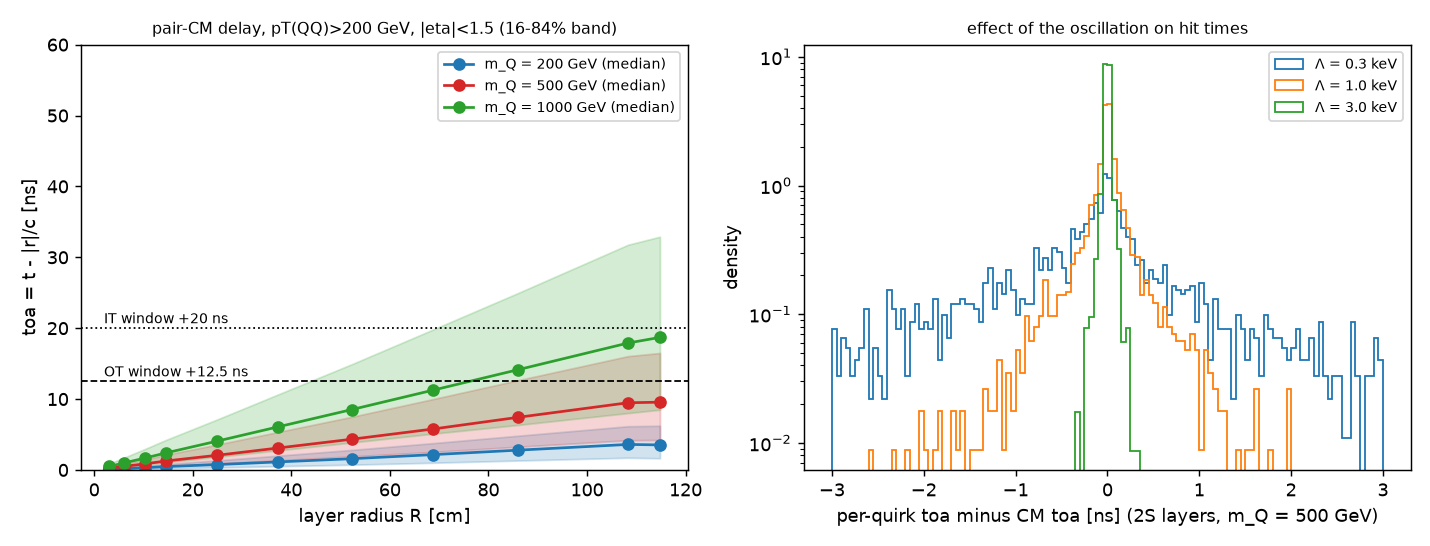
\includegraphics[width=0.95\textwidth]{figures/T3_timing.png}
\caption{\textbf{Hit timing of slow pairs} \src{T3 \S6; \file{code/T3_timing.py}; \EST{}; exact kinematics}. Left: pair-CM arrival delay $t-|r|/c$ vs layer radius (median and 16--84\% band) with the IT ($+20$\,ns) and OT ($+12.5$\,ns) windows. Right: per-quirk spread around the CM delay in the 2S layers at 500\,GeV for $\Lambda=0.3$, 1, 3\,keV.}\label{fig:T3timing}
\end{figure}

\subsection{Trajectory model and measurement}\label{sec:traj}
\subsubsection{Degeneracy theorem and measuring \texorpdfstring{$(\mQ,\Lambda)$}{(mQ, Lambda)} after a discovery \src{S-4}}
\textbf{Theorem.} Hits, hit times and dE/dx depend on $(\mQ,\Lambda)$ only through $\ell_0=\mQ/\sigma$ and the velocities. It follows exactly from the scale invariance of the NG + point-mass action (vacuum Fisher column for $\ln\sigma$ $\le3\times10^{-7}$ of the largest) and was confirmed independently by dimensional analysis [R1 \S3]. Only three things break it: the recoil (MET $=\pTQQ$), the B field through $\varepsilon_B=qB/\sigma$, and material ($\propto1/\mQ$).

\begin{center}\small
\begin{tabular}{@{}L{3.2cm}L{3.7cm}L{3.8cm}L{4.6cm}@{}}\toprule
Handle & per event & $N=30$, statistical & $N=30$, with 1--3\% MET/JES scale\\\midrule
+MET ($\sigma_\perp=25\GeV$) & $\sigma(m)/m$ 6--10\%, $\sigma(\Lambda)/\Lambda$ 3--5\% & 0.9--1.2\% / 0.5--0.6\% & \textbf{$\approx$1--3\% / 0.5--1.5\%}\\
B only (no recoil) & $\sigma(\Lambda)/\Lambda$ 16--20\% at 1\,keV & 1.5--2.2\% (1\,keV); 17--29\% (3\,keV); none at 10\,keV & needs $q$ known and the crossing physics modelled to $\lesssim10\%$\\\bottomrule
\end{tabular}\end{center}
Caveats: local Cram\'er--Rao bound, known hit-to-quirk assignment, no PU, global minimum assumed (aliasing at 10\,keV); PUPPI $\sigma_\perp$ at PU 200 \UNV{} (scanned 15--35\,GeV); the pair's own $\lesssim5\GeV$ calorimeter deposit biases MET by $\lesssim2\%$ (correctable). The natural real tool is simulation-based inference trained on \file{T3_causal.py} events (suggestion, not studied). \textbf{This corrects published expectations}: a trajectory fit, dE/dx, crossing spacing or timing cannot measure $\mQ$ or $\Lambda$ alone (Section~\ref{sec:disc}).

\begin{figure}[!htbp]\centering
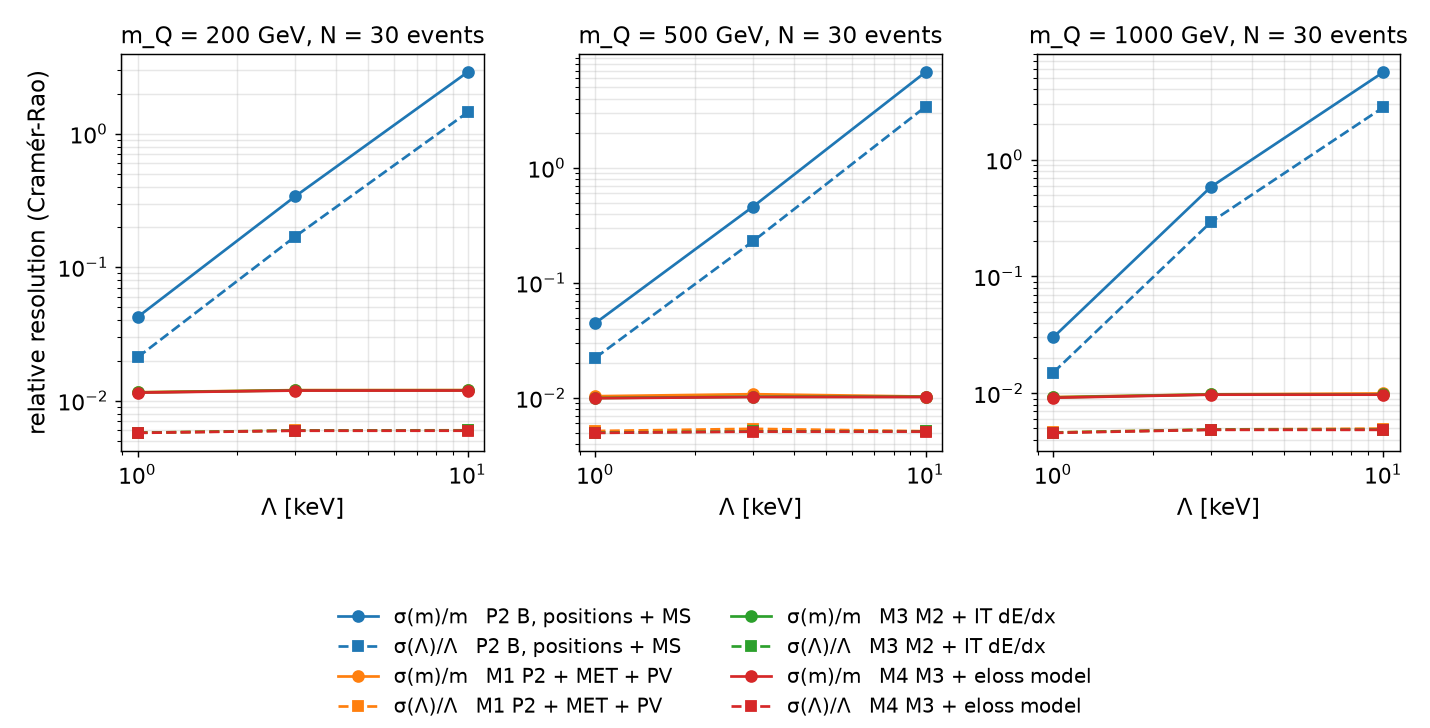
\includegraphics[width=0.97\textwidth]{figures/T4_fisher_summary_rep.png}
\caption{\textbf{Cram\'er--Rao resolutions for 30 events} \src{T4 \S4.3; \file{code/T4_fisher.py}, \file{code/T4_fisher_report.py}; \EST{}, idealised}. Solid: $\sigma(m)/m$; dashed: $\sigma(\Lambda)/\Lambda$. Blue: positions + MS with the B field only (no recoil); orange/green/red (overlapping): adding MET and the PV, IT dE/dx, and an energy-loss model. Statistical only: the 1--3\% MET-scale floor is not included. Re-plotted from \file{figures/T4_fisher_summary.npz} with larger fonts.}\label{fig:T4fisher}
\end{figure}

\begin{figure}[!htbp]\centering
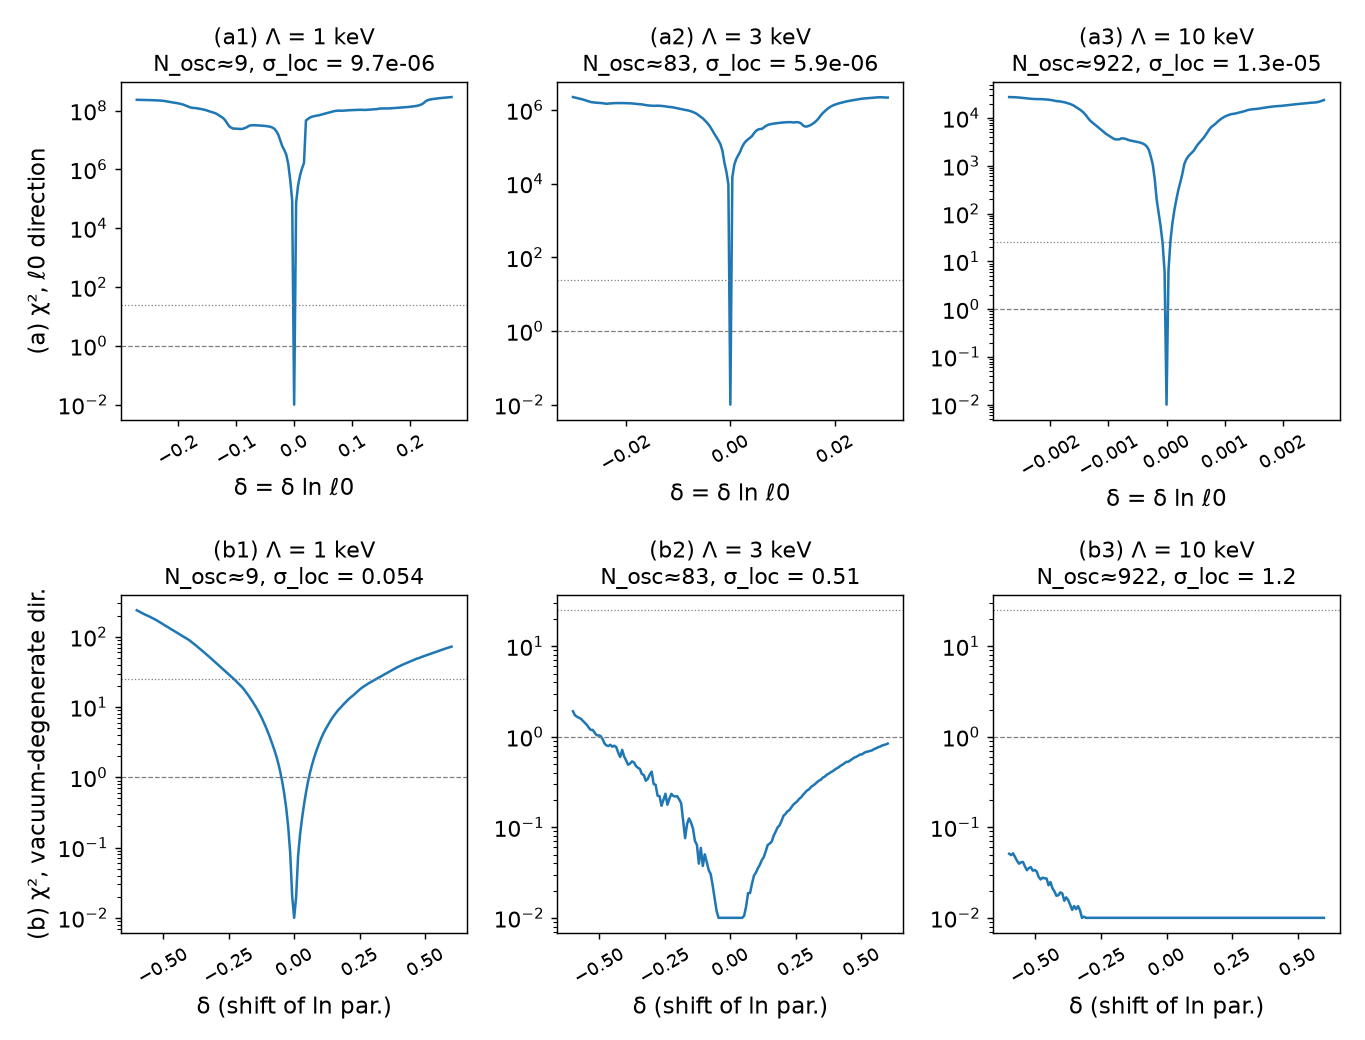
\includegraphics[width=\textwidth]{figures/T4_comb_rep.png}
\caption{\textbf{Linearity of the causal hit model} \src{T4 \S2.4; \file{code/T4_comb.py}; \EST{}; one event, 500\,GeV, no MS}. Top: $\chi^2$ along the oscillation-scale direction $\delta\ln\ell_0$ at fixed velocities, a very narrow ``comb'' minimum (phase-sensitive; aliasing at 10\,keV). Bottom: along the vacuum-degenerate direction ($d\ln m=d\ln p_T=2\,d\ln\Lambda$), constrained only by the B field and flat at 10\,keV. The linear window is a few per cent of a cycle: no Kalman filter; a global fit with a phase-scan seed. Panels (a1)--(a3) and (b1)--(b3) re-plotted from \file{figures/T4_comb.npy} (top-row $x$ axis: $\delta\ln\ell_0$ at fixed velocities).}\label{fig:T4comb}
\end{figure}

\subsubsection{MET-strip alignment \src{S-5}}
\textbf{Credit:} proposed qualitatively by Knapen et al.\ (``can easily be removed through either a $\Delta\phi$ requirement between $\not\!\!E_T$ and $n_3$'' [1708.02243 \S IV]; also Kang--Luty \S4.1). \textbf{New:} in vacuum the strip axis is exactly $\phi_{\rm pair}$; the B wobble ($\lesssim2\times10^{-4}$\,rad) and fit error ($3\times10^{-5}$\,rad) are negligible, so $\Delta\phi$(MET, strip) is set by the MET resolution. $|\Delta\phi|<0.15$--0.25\,rad keeps 95\% of the signal and rejects \emph{isotropic random planes} by $\pi/\delta_{95}=\times13$ ($\sigma_\perp=35\GeV$) to $\times34$ ($\sigma_\perp=15\GeV$). The seeding road is the same wedge (do not multiply). Against the real background (\EST{}, qualitative): $\times13$--34 per fake candidate for PU/UE planes, but only $\times\approx1$--3 for W($\tau\nu$)/lost-lepton events, where the visible object and the MET are collinear. \textbf{Do not put $\times13$--34 into a background estimate.}

\begin{figure}[!htbp]\centering
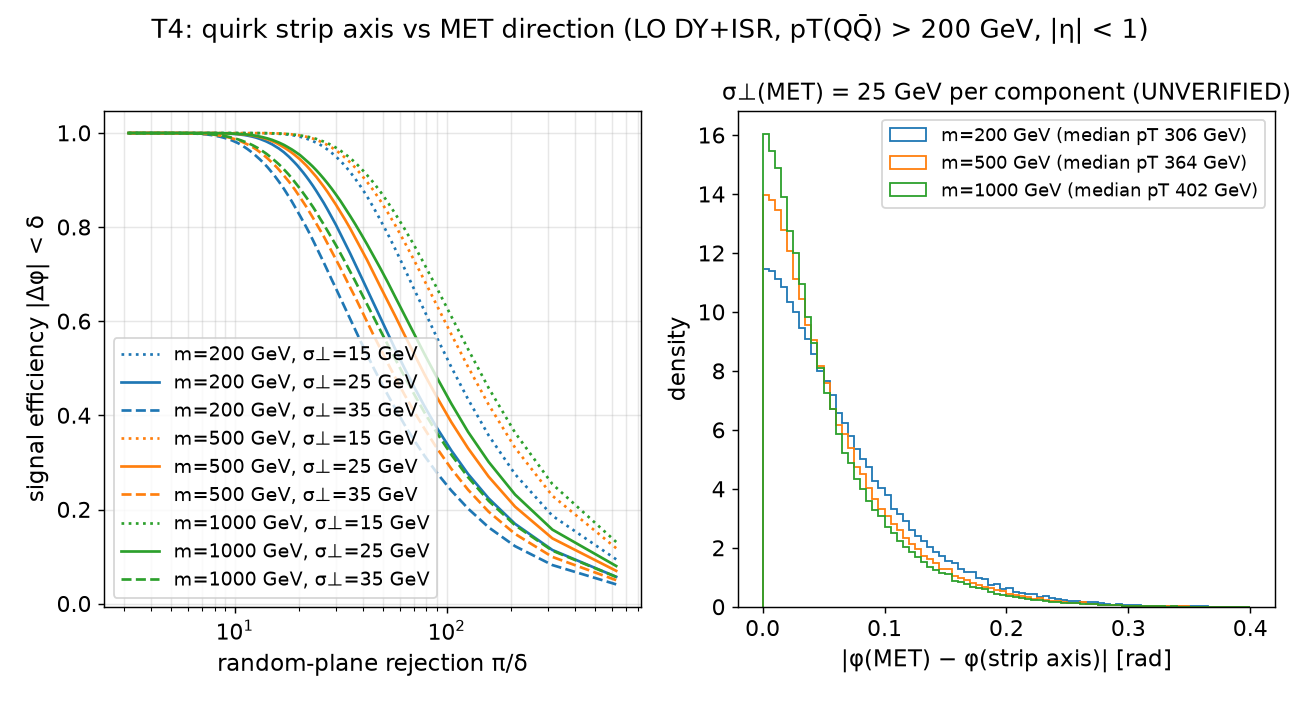
\includegraphics[width=0.97\textwidth]{figures/T4_met_alignment_rep.png}
\caption{\textbf{Strip axis vs MET direction} \src{T4 \S5.1; \file{code/T4_met.py}; \EST{}}. Left: signal efficiency vs rejection of isotropic random planes for three masses and $\sigma_\perp=15/25/35\GeV$ per MET component (\UNV{} PU-200 resolution). Right: $|\phi({\rm MET})-\phi({\rm strip})|$ for $\sigma_\perp=25\GeV$. Random planes only; the real-background gain is unknown.}\label{fig:T4met}
\end{figure}

\subsubsection{Global fit, seeding and trigger features \src{S-7, S-18}}
\begin{itemize}
\item \textbf{Credit:} Sha et al.\ already fit tracks under a quirk vs a helix hypothesis with a $\chi^2$ ratio (94\% of quirks kept at 500\,GeV, 0.5\,keV; all SM tracks in their sample removed) [2410.00269 \S V]; Knapen et al.\ proposed fitting a quirk trajectory [1708.02243 \S IV].
\item \textbf{New:} a 9-parameter causal \emph{pair} fit ($z_0$, $P_{Q\bar Q}$, $\gst$, CM axis, $\mQ$, $\Lambda$) plus MS kinks, against 50--130 measurements; linear only within 2--10\% of a cycle at the last layer, so a global Gauss--Newton fit with a phase-scan seed, not a Kalman filter. Seeding: resolved arcs for $\Lambda\lesssim1\keV$, an aliased zig-zag band through the PV for $\Lambda\gtrsim3\keV$; the pair separation is non-monotonic in $r$ in 98--100\% of events.
\item \textbf{Predictive power (idealised upper bound)}: an OT hit predicted from the IT has a 15--55\um\ uncertainty against 0.5--24\,mm strips: at most $\times20$--100 per OT layer at 1\,keV, $\times2$--10 at 3\,keV, none at 10\,keV. OT misalignment ($\approx10$--30\um, \UNV{}) and PU-200 hits reduce it; \textbf{do not quote it as a background reduction}.
\item \textbf{L1:} only 23--47\% of quirk OT crossings form 2\,GeV stubs at $\Lambda\le3\keV$ (76--89\% at 10\,keV), and they do not form helices; the trigger is L1 MET.
\item \textbf{Mean energy loss} is a first-order trajectory effect: OT hits shift by 40--180\um\ (200--500\,GeV) and 0.3--1.5\,mm (1\,TeV); a 10\% material error moves them by 4--150\um\ \src{S-12}.
\end{itemize}

\begin{figure}[!htbp]\centering
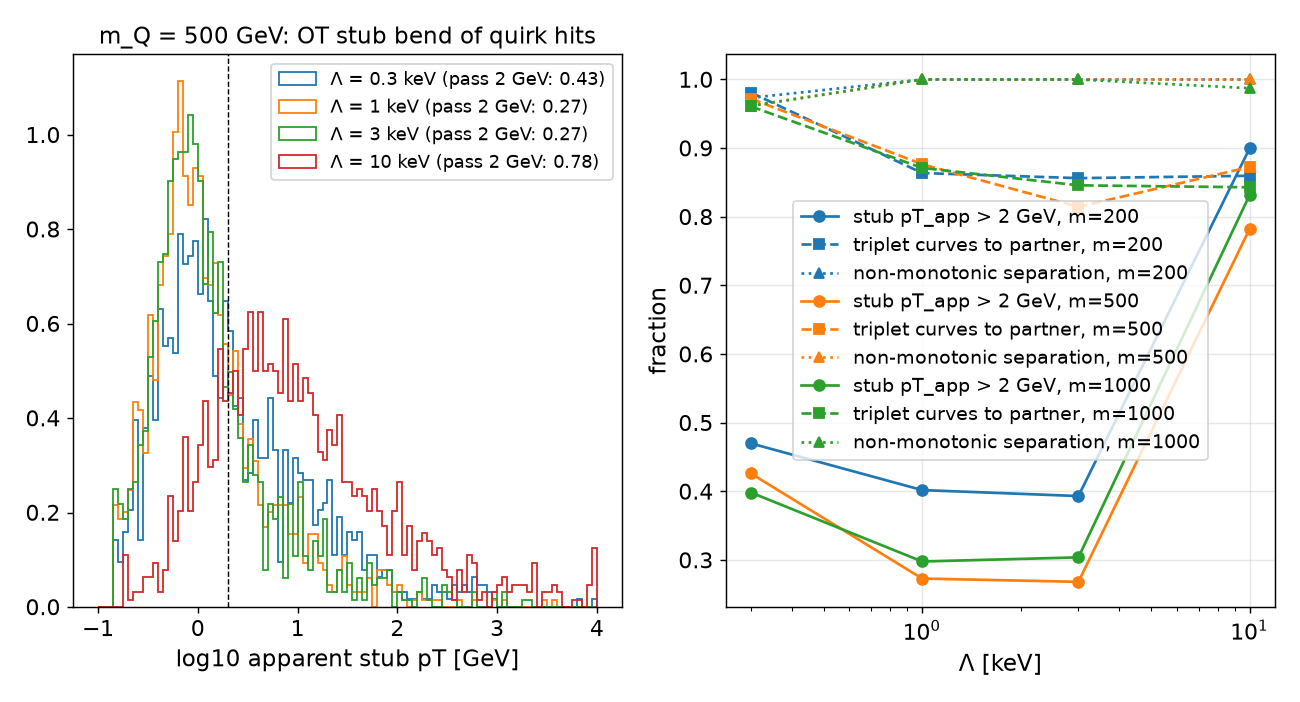
\includegraphics[width=0.97\textwidth]{figures/T4_local_rep.png}
\caption{\textbf{Local signatures} \src{T4 \S5.3, \S6; \file{code/T4_local.py}; \EST{}; no material}. Left: apparent stub $p_T$ of OT quirk hits at 500\,GeV (dashed: 2\,GeV stub threshold). Right: fraction of crossings passing the 2\,GeV stub cut, fraction of hit triplets curving towards the partner, and fraction of events with non-monotonic pair separation, vs $\Lambda$. Module spacings \UNV{}.}\label{fig:T4local}
\end{figure}

\subsection{Other exploitable gaps}\label{sec:other}
\begin{description}[leftmargin=0.4cm,style=nextline]
\item[S-9 Athena step-count killer (do first)] \file{QuirksPreInclude} attaches \texttt{MonopoleLooperKiller} with \texttt{MaxSteps}$=2\times10^6$ (BSM only). The quirk stepper takes $\approx150$--200 Geant4 steps per crossing and $N_{\rm cross}\approx24(\Lambda/\keV)^2$ in a CMS-size tracker, so a naive port kills quirks inside the tracker for $\Lambda\gtrsim24\keV$ (\EST{}). FASER ($\approx10^5$ crossings at 100\,keV): possible, \UNV{}. SREQ W1(v) already asks for an exemption; this quantifies why. A configuration note, hours.
\item[S-10 Merged pair 9--21$\times$ MIP] An HSCP-like high-$\Lambda$ category (IT ToT, MTD $1/\beta$, OT HIP bit); distinguishable from $|q|=2$ only with $\beta$. A CMS HSCP recast needs care: the merged pair is net neutral, so its ``track'' is straight. IT ToT saturation \UNV{}.
\item[S-11 Conventions and closed forms] Documentation; hours (Tables~\ref{tab:boxA}, Section~\ref{sec:osc}).
\item[S-12 Mean energy loss] A fit nuisance and efficiency systematic for any $\chi^2$/GNN using OT positions (\WAC{}).
\item[S-13 ISR tail] Two groups differ by 37\% in mass reach on one benchmark largely from ISR/K-factor handling; FASER needed an ISR reweighting. Already planned in STRATEGY \S12; add ``never a fixed-$p_T$ kick''.
\item[S-14 GUT ladder and doublet invisibility] Doublet charged members decay with $c\tau=7.8$\,mm, so the pair is neutral before the first pixel layer (survival to 3\,cm $\le0.2\%$ at 200\,GeV). The theory-favoured representation gives monojet + soft displaced pions at $\times14$ the $E$ rate (84\,fb at 500\,GeV): a compressed-higgsino-style monojet recast (limits not opened, \UNV{}). Drop the ``2 $L$ points as a tracker topology test'' (OQ Q4).
\item[S-15 Cosmology] Credit: the implication ``discovery $\Rightarrow$ low reheating'', including $T_{\rm RH}\lesssim\mQ/25$, is the headline of \cite{cool}. Ours: window numbers 5--40\,GeV with the SU(2) conversion; $\Omega\propto T_{\rm RH}^{21/4}$ (not $T^7$); an unresolved $\times2.2$ (Section~\ref{sec:disc}).
\item[S-16 $\Lambda\gtrsim3\MeV$ and the 0.1--3\,MeV band] Prompt resonance at $2\mQ$ [0805.4642 \S5, Eq.5.59] with $\sigma\times{\rm BR}(\ell\ell)=1.1\fb$ at 500\,GeV; ATLAS dilepton limits probably exclude $\mQ\lesssim0.8$--1\,TeV (a reading, \UNV{}). Displaced annihilation at 3\,cm--10\,km for 0.1--3\,MeV (using [1811.08903 Eq.4.4]): no search. The tracker search should not claim $\Lambda\gtrsim1\MeV$.
\item[S-17 $|q|=2$ singlets] $\sigma\propto q^2$ ($+18$--21\% from $\gamma\gamma$); tracker reach $\approx1.3\TeV$ vs 1.15\,TeV. With the causal scaling ($\Ds\propto qB/\Lambda^{1.9}$) $\Lambda_{\rm low}$ rises by $\approx2^{1/1.9}\approx1.4$, not $2^{1/4}$; MS floor doubles to 22--44\um; dE/dx $\times4$ (\EST{}).
\item[S-18 Trigger, PU 200, PU-vertex association, HLT] Experimental; months. The plane fit's $z_0$ is known to $\approx30$--60\um\ from the IT; $\approx30\%$ of events have another PU vertex within $\pm100\um$ (\EST{}). This is a background handle (fake planes point to their own vertex), not a signal ambiguity.
\item[S-19 $\varepsilon$ (glueball emission per crossing)] $\varepsilon=0.1$ has no derivation; emission needs $b<1/\Lambda$, which in 3.8\,T applies to no crossing for $\Lambda\lesssim2\keV$, the even crossings for 3--20\,keV, all above $\approx30\keV$. Irrelevant for CMS; could relax FASER's 30--100\,keV limits (low priority).
\item[S-20 Exclusive $\gamma\gamma\to Q\bar Q$ with PPS] $\approx35$ produced events at 500\,GeV with PPS-2 acceptance; a post-discovery mass handle independent of the MET scale. Inelastic $\gamma\gamma$ adds only 4.0--4.2\% (killed as a boost).
\end{description}

\subsection{Ranked gap list S-1 \ldots\ S-20}\label{sec:ranked}
Ranking criterion: (impact on the CMS search or on constraints) $\times$ confidence $\div$ remaining effort \src{synthesis \S1}. Type: \textbf{C} correction to the existing plan; \textbf{N} new capability; \textbf{Ch} new or complementary channel; \textbf{D} documentation. The last column separates what this track adds from what was already published (credits added after R2--R3).
{\footnotesize
\begin{longtable}{@{}L{0.45cm}L{0.75cm}L{4.0cm}L{2.1cm}L{1.45cm}L{1.15cm}L{5.35cm}@{}}
\caption{Ranked gaps (synthesis v4 \S1). IDs unchanged since v1.}\label{tab:ranked}\\
\toprule \# & ID / type & Gap and best number(s) & Verdict & Effort & Conf. & New here vs.\ already in the literature\\\midrule\endfirsthead
\toprule \# & ID / type & Gap and best number(s) & Verdict & Effort & Conf. & New here vs.\ already in the literature\\\midrule\endhead
\bottomrule\endfoot
1 & S-1\newline N+C & Causal NG string validated (0.990--1.004 vs indep.\ solver); Li 3--35\% low if converged ($\gst$-dep.); printed step unconverged; lab slices $\times1.5$--75 & \EXPL{} (adopt \file{T3_causal.py}) & days & high & New: independent validation; converged, $\gst$-binned Li comparison; convergence requirements. Already: the causal construction (Athena/Lund; used by ATLAS/FASER); Li et al.'s own warning that $\hat s$ matters [2002.07503 \S VIII]\\
2 & S-6\newline C & Timing medians 3.5/9.6/18.7\,ns; 2S lost 7--33\% (500\,GeV), 44--68\% (1\,TeV); $\approx3$ hits/layer & \EXPL{} & done & high & New for CMS Phase-2 with the triggered spectrum. Li Tab.I already gives 37\% with $>2$ hits at 500\,GeV\\
3 & S-3\newline C+N & $\Ds_B\propto\Lambda^{-1.6\ldots-2.0}$, $\mQ$-indep., $B\ln(1/B)$ at crossings; window 0.45--0.7\,keV (truth) & \EXPL{} (window, V2); \WAC{} (analytic) & 1--2 wk & med.--high & New: converged exponents, $B$ non-linearity and its crossing origin, corrected window. Already: mild $m$ dependence, $\sim\Lambda^{-2}$, $\propto q$, formula only order-of-magnitude [2002.07503 \S V, App.C]\\
4 & S-2\newline C+N & MS floor 11/15/22\um\ (truth); per-hit $\sigma_n$ IT 17\um, PS 0.25\,mm, 2S 8\,mm & \EXPL{} & days & medium & New: CMS Phase-2 quantification. Already: Athena/FASER G4 uses standard EM processes; Knapen evaluated $\Ds$ on detector-level hits\\
5 & S-4\newline N & Degeneracy theorem; 1--3\% ($\mQ$), 0.5--1.5\% ($\Lambda$), 30 events & \EXPL{} & days / wks & high / med. & New: theorem and first quantitative answer. Shows that the 2108.06748 \S5 statement and Knapen's expectations are not supported by the theorem\\
6 & S-5\newline C+N & MET-strip: $\times13$--34 vs \emph{random} planes at 95\% & \EXPL{} & days & high (geom.), low (gain) & Proposed by Knapen \S IV and Kang--Luty \S4.1; new: the 95\% window, rejection, real-background analysis\\
7 & S-9\newline C & Athena MaxSteps $2\times10^6$ kills quirks for $\Lambda\gtrsim24\keV$ & \EXPL{} (config) & hours & medium & New (code reading of Athena)\\
8 & S-8\newline Ch & Stopped pairs: $f_{\rm stop}$(EB+HB) $1.0\pm0.3\%$; HL-LHC 0.3--0.55\,TeV; Run-2+3 update 0.15--0.35\,TeV & \EXPL{} (complement.); \WAC{} (update) & weeks & med.--low & Already: the recast itself, trigger fraction, 300\fbinv\ projections [1811.08903]. New: causal $f_{\rm stop}$, triggered-sample $f_{\rm stop}$, 3\abinv\ projection with a background bracket, Run-2+3 estimate\\
9 & S-10\newline C+Ch & Merged pair 9--21$\times$ MIP & \EXPL{} (corr.); \WAC{} (recast) & days & medium & D0 used the same per-trajectory method [1008.3547]; new: the CMS central-sample numbers\\
10 & S-7\newline C+N & 9-par.\ causal global fit; OT prediction 15--55\um\ (idealised) & \EXPL{} (approach) & weeks & medium & Already: quirk vs helix $\chi^2$ [2410.00269 \S V]; trajectory fit idea [1708.02243]. New: causal pair fit, linearity/aliasing, predictive power, seeding\\
11 & S-11\newline D & Conventions; closed forms; scalar $\times1.7/\times0.81$ & \EXPL{} & hours & high & New: lattice-based table and closed forms\\
12 & S-12\newline C & Mean energy loss shifts OT hits 40\um--1.5\,mm & \WAC{} & days & medium & Already: ionisation force in the EoM (Li; 2108.06748); new: OT-hit shift numbers\\
13 & S-13\newline C & ISR tail: fixed-$p_T$ trick biases $\lmax$ $-10$--25\% & \EXPL{} (planned) & weeks & high & 37\% reach spread noted by T5 from published numbers\\
14 & S-14\newline Ch & GUT ladder (doublets); doublets invisible; monojet recast & \EXPL{} (lines); \WAC{} (recast) & days & med.\ / low-med. & Ladder from Kang--Luty/Martin; new: SU(2)/SU(3) strips and the invisibility consequence\\
15 & S-15\newline D+C & Reheating implication; $T_{\rm RH}\lesssim5$--40\,GeV; $T^{21/4}$; $\times2.2$ & \EXPL{} (figure); \WAC{} (note) & days & medium & Already: the implication and $T_{\rm RH}\lesssim\mQ/25$ [2512.20696]. New: window numbers, scaling, normalisation check\\
16 & S-16\newline Ch & $\Lambda\gtrsim3\MeV$ resonance (prob.\ excluded to 0.8--1\,TeV, \UNV{}); 0.1--3\,MeV band & \EXPL{} (scoping); \WAC{} & days & low & Resonance from Kang--Luty \S5; annihilation length from E--L Eq.4.4\\
17 & S-17\newline Ch & $|q|=2$: $\sigma\times4$, reach 1.3\,TeV, $\Lambda_{\rm low}\times1.4$ & \WAC{} & days & medium & Uses Li's $\propto q$; new: causal scaling of $\Lambda_{\rm low}$\\
18 & S-18\newline N & Trigger, PU 200, PU vertex, HLT; L1 stubs 23--47\% & \WAC{} (exp.) & months & medium & PU 200 never simulated for a quirk tracker analysis\\
19 & S-19\newline N & $\varepsilon$ active only for $b<1/\Lambda$ & \WAC{} (low) & weeks & low & Criterion from E--L App.B.1; new: crossing-by-crossing application\\
20 & S-20\newline N & Exclusive $\gamma\gamma$ + PPS: 35 events at 500\,GeV & \WAC{} (post-disc.) & weeks & medium & New estimate\\
\end{longtable}
}

\subsection{Cross-report tensions and how they were resolved}
{\footnotesize
\begin{longtable}{@{}L{0.7cm}L{5.4cm}L{10.2cm}@{}}
\caption{Tensions between investigator reports (synthesis \S2; called T-n in v1).}\label{tab:tensions}\\
\toprule ID & Tension & Resolution\\\midrule\endfirsthead
\toprule ID & Tension & Resolution\\\midrule\endhead
\bottomrule\endfoot
X-1 & ``precession is not a $\Lambda$ meter'' (T3) vs ``in-plane B displacement is a recoil-free $\Lambda$ meter'' (T4) & different observables: T3 killed the secular rigid rotation (3--18\,$\mu$rad $<$ MS 4.5--10\,$\mu$rad); T4 uses the whole non-rigid pattern $x_B\approx0.5\varepsilon_BR$. T2's $\Lambda^{-2.5}$ (4 events, unconverged causal column) retired\\
X-2 & causal $\Lambda^{-1.6\ldots-2.0}$ vs formula $\mQ/\Lambda^4$ & the formula is the odd-crossing miss distance; first-order perturbation theory fails at crossings; ``$\times7$--50 at 3\,keV'' already in Li App.C\\
X-3 & causal string non-linear in B (T4, artefact not excluded) & confirmed by S (converged) and R1 (independent solver); exactly linear before the first crossing\\
X-4 & $\Lambda$ convention 0.709 (T1), 0.71 / ``15\%'' (T5) vs $1/0.6$ (TH) & T1 and T5 agree; 15\% on $\Lambda$, 18\% inverted, 28\% on $\sigma$; $\le4\%$ effect on cosmology\\
X-5 & $f_{\rm stop}$ 1--6\% (T6) vs $1.0\pm0.3\%$ (T3) & different fiducial definitions; T6 took Evans--Luty $\times3$; T3 computed it\\
X-6 & timing medians (T3) vs strategy 16/33\,ns & strategy right for fixed $p_T=250\GeV$; the triggered spectrum gives 9.6/18.7\,ns\\
X-7 & MS 50--400\um\ (T5) vs 11--22\um\ (T3) & T3 supersedes T5's upper bound (plane fit, kick sharing, restoring dynamics)\\
X-8 & $\Lambda$ from crossing period / BTL double hits (T2, T3) vs degeneracy theorem (T4) & T4 right: these measure $\ell_0$, never $\Lambda$ alone\\
X-9 & GUT-favoured $\Lambda$ (T1) vs tracker visibility (T3, T6) & a tension in motivation: the ladder predicts invisible doublets\\
X-10 & $|q|=2$ window (T6) vs causal scaling (T3) & $\Lambda_{\rm low}$ rises by $\approx1.4$, not 1.19\\
X-11 & ``10--20\% of events with $>2$ hits'' (strategy, from Li Tab.I) vs $\approx3$ hits/layer & Li Tab.I itself gives 37\% at 500\,GeV; the strategy took lighter, faster points\\
X-12 & MET alignment $\times5$--10 (T5) vs $\times13$--34 (T4) & T4 computed the 95\% window; against random planes only\\
X-13 & straight string ``good to 1--4\%'' (TH \S3.1) vs ``uncontrolled at O($F_{\rm ext}$)'' (T2, T3) & TH bounds angles, not observables; the error depends on the prescription: Li converged $-3\ldots-35\%$ ($\gst$-dep.), labSS $\times1.5$--75, Li at printed step $\times0.8$--20. The causal string is the reference; the comparison is superseded, not a systematic\\
\end{longtable}
}

\subsection{What the checks did and did not test}
The v1 synthesis announced ``35/35 PASS''; that was 30 assertions in \file{S_spotchecks.py} plus five rows, and \textbf{none} compared a published integrator or an independent string solver with the causal string, so the premise of the v1 top gap was never tested \src{\S3.0; R1 A-3}. The final table has 23 rows: rows 1--21 (v2) split into 12 independent closed-form or independent-code checks, 5 same-code-new-sample checks, 3 re-runs and one new-model estimate; rows 22--23 (added in v3) are independent runs by R2. Two v1 premises \textbf{fail}: ``labSS represents Li et al.''\ (row 15: labSS/Li = 1.6--73) and ``straight string + MS gives fake mm thickness'' (row 19: holds for labSS only). One v2 statement fails as a general statement: ``Li $\approx15\%$ low'' (row 22: depends on $\gst$). \textbf{Still untested:} the Athena C++ itself, the Knapen--Papucci code, the Phase-2 material, anything with PU, the analytic coefficient of the $B\ln B$ term, and the $f_{\rm stop}$ numbers (not re-run by anyone).

% ======================================================================
\section{Discrepancies found in the literature and in public code}\label{sec:disc}
This chapter collects every place where the track found a published statement, a public code setting, or a number in our own project documents that disagrees with a check. ``Size'' is the size of the disagreement on the quantity stated. Status: \VER{} = established by independent code, a closed form or a direct reading of the primary text by at least one reviewer; \EST{} = our calculation with a single code; \UNV{} = not established (figure reading, recalled, or code not seen). \textbf{Credit is given where the authors themselves noted the issue.}

\subsection{Published papers}
{\footnotesize
\begin{longtable}{@{}L{2.2cm}L{3.4cm}L{4.4cm}L{2.0cm}L{1.3cm}L{1.9cm}@{}}
\caption{Discrepancies with published papers.}\label{tab:disclit}\\
\toprule Source & Claim / setting & What we found & Size & Conf. & Status\\\midrule\endfirsthead
\toprule Source & Claim / setting & What we found & Size & Conf. & Status\\\midrule\endhead
\bottomrule\endfoot
2512.20696 (Asadi, Kribs, Luty) Eq.1, \S2 & $\Lambda\equiv T_c=0.6\sqs$; $m_0=6T_c$ & lattice SU(2): $T_c/\sqs=0.709$ [hep-lat/0307017 Tab.6; 0912.3339 Eq.33]; 0.6 is the $N\to\infty$ value. Their ``1\,keV'' is $\sqs=1.41\keV$ (not 1.67); $m_0=5.33T_c$ (theirs 13\% high). Their length formula keeps the collider coefficient while defining $\Lambda=T_c$: a convention trap (lengths $\times2.0$ if read literally) & 15\% on $\Lambda$, 28\% on $\sigma$; $\le4\%$ on $T_{\rm RH}$ & high & \VER{} (S check 5; T1, T5 agree)\\
2512.20696 \S4.2 & relic abundance $\Omega\propto T_{\rm RH}^7$ & once the frozen-in gluons self-thermalise ($\Gamma_{2\to3}/H\sim10^{10}$ at the bound) the scaling is $T_{\rm RH}^{21/4}$ (numerically $T^{5.0}$ with $g_{*s}$); a $\times100$ abundance uncertainty moves $T_{\rm RH}$ by $\times2.5$, not ``at most $\times2$'' & exponent 5.25 vs 7 & medium-high & \VER{} (analytic; S and R1 agree)\\
2512.20696 Fig.4 & $T_{\rm RH,max}$ at $\mQ=600\GeV$, $T_c=1\keV$: 15\,GeV (overclosure), 6.4\,GeV (SIDM) & T1 gets 33 and 16\,GeV; slopes agree; a missing $g_{*s}$ dilution would explain $\times1.8$ & $\times2.2$ in $T_{\rm RH}$ ($\times50$ in $\Omega$) & low & \UNV{} (their code is not public; contact authors before claiming an error)\\
1911.02223 Eq.III.10 (Li, Li, Pei, Zhang) & Euler step ``should satisfy'' $\epsilon<10^{-4}$\,ns $\times(\mQ/100\GeV)$ $\times(\keV/\Lambda)^2$ & at this bound the integration is not converged: thickness $\times0.8$--20 (0.6--3\,keV), OT hits 6--250\,mm off; convergence needs $10^{-2}$--$10^{-3}$ of it, shrinking $\propto\Lambda^{-2}$. The step they actually used is unknown, so the impact on their published reach is unknown & up to $\times20$ in $\Ds$ & high (for the bound) & \VER{} (R1, F1, R2 independent code)\\
1911.02223 Eq.III.12 & $d=1.16\um$ $\times(\mQ/100\GeV)$ $\times(\keV/\Lambda)^4$ $\times(B/{\rm T})$ & the plane-fit thickness scales as $\Lambda^{-1.6\ldots-2.0}$, $\mQ$-independent; the formula is the odd-crossing miss distance. \textbf{Already noted by Li et al.}\ themselves [2002.07503 App.C, Fig.8: $10^{-3}$--$10^3$ scatter; their reach uses the numerical thickness]. It is our strategy that used the formula & $\times7$--50 at 3\,keV; $\times100$+ at 10\,keV & high & \VER{} (two NG solvers)\\
1911.02223 / 2002.07503 (Li method) & CM-simultaneous straight string (no retardation, no curvature) & vs exact causal string, converged: $\Ds$ low by $\approx3\%$ ($\gst\approx1.05$), 15\% (1.3), 30--35\% (2--3); single events $-47\%\ldots+36\%$; out-of-plane hit differences up to 124\um. Evans--Luty's ``retarded time corrections \ldots\ safely neglected'' [1811.08903 \S2] and Kang--Luty's call for a direct check [0805.4642 \S3.2] are thereby answered for the thickness & 3--35\% (me\-dian, $\gst$-dep.) & high at $\gst=1.28$; medium else\-where (5 events per point) & \VER{} (R1, R2)\\
2002.07503 \S VIII, Fig.6 & fixed $\hat s$ changes $\Ds$ from $\sim100\um$ to several mm & confirmed: fixed $\hat s$ has no transverse restoring force once $F_{\rm ext}\ne0$; \textbf{Li et al.\ already said so} (``choosing the correct $\hat s$ direction is critical'') & -- & high & \VER{} (agreement)\\
2108.06748 \S5 (Li, Pei et al., FASER) & ``after obtaining the oscillation amplitude and oscillation period \ldots\ one can infer the confinement scale, quirk mass'' & amplitude and period carry only $\mQ/\Lambda^2$ and velocities (their own Eq.4.18 is consistent with this), so they fix $\ell_0$, not $\mQ$ and $\Lambda$ separately, without the recoil & qualitative & high (theorem) & \VER{} (R1 dimensional analysis; R4 text check). ``Not supported'', softened from ``refutes''\\
1708.02243 \S IV, App.A (Knapen et al.) & fitting a quirk trajectory is ``an obvious way to try to measure the mass and string tension''; dE/dx ``will be important to measure the mass and string tension'' & by the same theorem, positions and dE/dx measure $\ell_0$ and $\beta\gamma$ only; adding IT dE/dx changes $\sigma(\mQ)$ by 0\% & qualitative & high & \VER{} (T4 Fisher; R1)\\
1708.02243 Fig.6 vs 1911.02223 App.A, Fig.9 & reach for coloured $D^c=(3,1)_{2/3}$, 300\fbinv, coplanar: 1500 vs 2050\,GeV & same benchmark, same observable, +37\% in mass; Li et al.\ cite an ``incorrect cross section''; the LO $pp\to DDj$ ($p_T>200$) cross section exceeds $pp\to DD$ for $m>500\GeV$ (Knapen's own trigger efficiencies are 0.24 for $D^c$ and 0.10 for $E^c$, so the 0.24 vs 0.10 is a channel difference, not a Knapen--Li difference). Shows how fragile LO + shower ISR modelling is & +37\% in $\mQ$ & medium & read in the papers by T5; cause not resolved\\
same pair & $E^c$ reach, 300\fbinv: 650 (Knapen) vs 500\,GeV (Li ``coincides well'') & probably 3-event (exclusion) vs 5-event (discovery) contours & 30\% & low & \UNV{}\\
same pair & plane-rotation / thickness scale for Knapen's benchmark ($\mQ=1.8\TeV$, $\Lambda=2\keV$, 2\,T) & Li's formula gives 2.6\um; Knapen's $\Delta\phi\times$ amplitude gives 0.45--13\um & $\times30$ spread & low & \EST{} (T5 arithmetic)\\
2002.07503 \S II.C & CMS field ``4\,T'' & CMS runs at 3.8\,T & 5\% & high & minor\\
1708.02243 & $\Lambda$ window ``100\,eV--30\,keV'' (abstract) vs ``100\,eV--10\,keV'' (text) & internal inconsistency & $\times3$ at upper edge & high & minor\\
Literature shorthands [2404.13814; 2607.26195; 2512.20696] & $\lmax\approx1$\,cm $\times(m/100\GeV)$ $\times(\keV/\Lambda)^2$; ``2\,cm$(\gamma-1)$'' & right on average near 500\,GeV but $\times0.4$--2.7 event by event; ``2\,cm$(\gamma-1)$'' is a factor 2 low & $\times0.4$--2.7; $\times0.5$ & high & \VER{} (closed form)\\
2404.13814, 2607.26195, 1811.08903 & $\varepsilon=0.1$ glueball emission per crossing, one number for all $\Lambda$, $\mQ$ & no derivation; emission needs $b<1/\Lambda$, which in 3.8\,T excludes all crossings for $\Lambda\lesssim2\keV$; Kang--Luty gave extremes $\sim1$ and $\sim10^{-3}$ & model choice & low & \EST{}\\
\end{longtable}
}

\subsection{Public code (GitLab / GitHub / Zenodo)}
{\footnotesize
\begin{longtable}{@{}L{2.9cm}L{3.0cm}L{4.5cm}L{1.7cm}L{1.1cm}L{2.1cm}@{}}
\caption{Findings on public code. Athena \texttt{main} read by T2 on 7 Oct 2026; the \file{Quirks} directory is snapshotted in \file{theory_track/data/athena_quirks_snapshot/}.}\label{tab:disccode}\\
\toprule Code & Setting & What we found & Size & Conf. & Status\\\midrule\endfirsthead
\toprule Code & Setting & What we found & Size & Conf. & Status\\\midrule\endhead
\bottomrule\endfoot
ATLAS Athena \file{Simulation/G4Extensions/Quirks} (\file{gitlab.cern.ch/atlas/athena}) & \textbf{causal string algorithm}:\newline \texttt{InfracolorForce},\newline \texttt{StringVector},\newline \texttt{HyperbolaStep} & \textbf{exact}: the absorb/emit map of null string vectors keeps $p^2=m^2$, composes exactly, and is the hyperbolic motion of a massive endpoint fed by a straight null segment: exact NG for piecewise-null data, causal, 4-momentum conserving. Python port: vacuum $\le2\times10^{-8}\lmax$, covariant to 0.05\um; independent solver agrees $\le1\%$ & no physics error found & medium-high & \VER{} for the algorithm (algebra + Python port + R1 solver); the C++ itself was \textbf{not run}\\
same, \file{QuirksPreInclude},\newline \texttt{G4UserActions-}\newline\texttt{Config.py},\newline \file{LooperKiller.cxx} & \texttt{Monopole-}\newline\texttt{LooperKiller},\newline \texttt{MaxSteps}$=2\times10^6$ (BSM only) & $\approx150$--200 G4 steps per crossing; $N_{\rm cross}\approx24(\Lambda/\keV)^2$ in a CMS-size tracker $\Rightarrow$ quirks killed inside the tracker for $\Lambda\gtrsim24\keV$. FASER: $\sim10^5$ crossings over 5\,m at 100\,keV, so possibly killed in the detector. The snapshot confirms the killer attachment (\texttt{MonopoleLooperKillerToolCfg}, \file{QuirksConfig.py} l.69); \texttt{MaxSteps}$=2\times10^6$ and \texttt{BSM\_Only} come from \file{G4UserActionsConfig.py} and \file{LooperKiller.cxx}, read by T2 on 7 Oct but not in the snapshot & tracks truncated above $\approx24\keV$ & medium & \EST{}; FASER configuration \UNV{}\\
same, \texttt{HyperbolaStepper} & \texttt{DistChord()} returns 0, \texttt{yerr}=0 (TODOs) & G4 chord-error control disabled; boundary crossings rely on the exact partial-absorption map plus G4's intersection tolerance (snapshot \file{HyperbolaStepper.cxx} l.80--86) & probably harmless & low & \UNV{} in ATLAS settings\\
same, field kick & kick then \texttt{m\_momentum *= mass/m\_momentum.m()} (``TODO: possible instability'') & first-order splitting error $O$(maxBoost) (snapshot \file{HyperbolaStep.cxx} l.116--117) & $\le1\%$ at maxBoost $10^{-2}$ & medium & \EST{} (port)\\
same, Geant4 material & ``standard Geant4 electromagnetic processes'' [2607.26195 App.A] & probably includes MS, which processes are attached was not checked; no MS effect on quirk observables is published & -- & -- & \UNV{}\\
Sha et al.\ samples (Zenodo 17941765; \file{shaqiyu/QuirkTracking-ML}) [2410.00269] & straight-string propagator, hits smeared by 1\,mm, no material & MS floor (11--22\um) certainly absent; string prescription and step unknown. If CM-simultaneous and converged: expect 3--35\% ($\gst$-dep.) thickness differences; if lab-slice or unconverged: mm-scale OT errors & unknown & -- & \textbf{validate against \file{T3_causal.py} before use as truth}\\
Knapen--Papucci propagator [1708.02243] & ``in the CM frame $v_\parallel$ lies along the displacement'' (\S II) & code not seen by anyone on the track & unknown & -- & \UNV{}; ask the authors\\
\file{burzynski-lab/quirk-tracking}, \file{quirkviz} (GitHub; ATLAS quirk search) & MaskFormer pair finder on Athena GNN4ITk dumps; displays default to 500\,GeV, 400\,eV & physics model is the Athena causal string, hence exact (S-1). The \texttt{MaxSteps} killer applies to any Athena sample unless exempted; whether their $\Lambda$ grid reaches $\gtrsim24\keV$ was not checked & -- & -- & not audited by this track (context: \file{research/samples_and_tools.md})\\
\file{eliwelch17/PreFASERQuirkSim} & C++17 port of the 2404.13814 forward transport (ionisation, LHC magnets, $\varepsilon$ weights) & forward-beamline specific; not audited by this track & -- & -- & not audited\\
\end{longtable}
}

\subsection{Our own project documents (pre-track numbers)}
{\footnotesize
\begin{longtable}{@{}L{3.0cm}L{4.0cm}L{5.3cm}L{1.5cm}L{2.0cm}@{}}
\caption{Numbers in the project's strategy and signal model that the track found wrong or in need of qualification. Proposed edits: Section~\ref{sec:mods}.}\label{tab:discown}\\
\toprule Document & Statement & What we found & Size & Status\\\midrule\endfirsthead
\toprule Document & Statement & What we found & Size & Status\\\midrule\endhead
\bottomrule\endfoot
\file{theory_signal_model.md} \S0(d), \S1.1, \S6.1 & convert the cosmology $\Lambda$ with $1/0.6$ (``$\sim1.7\keV$'') & use $1/0.709$ (SU(2)) or $1/0.646$ (SU(3)) & 18\% & \VER{}\\
TH \S3.1 & straight-string approximation ``good to $\lesssim1$--4\%'' & bounds the bending angles, not the observables; Li-type 3--35\% on $\Ds$, lab slices $\times1.5$--75 & 3--35\% & \VER{}\\
STRATEGY \S1, \S10.4 & median BTL delay $\approx16\ns$ (500\,GeV), 33\,ns (1\,TeV) & these are the 84th percentiles; medians 9.6/18.7\,ns (fixed $p_T=250$ vs real spectrum) & $\times1.7$ & \VER{} (closed form)\\
STRATEGY \S4.3, \S9.1, \S9.4 V4 & merged pair ``$\ge2\times$ MIP'' & FASER's forward-relativistic number; CMS central triggered: 9--21$\times$ MIP & $\times4.5$--10 & \EST{}\\
STRATEGY \S4.2 & ``1--5\% stop in the calorimeters'' & $1.0\pm0.3\%$ EB+HB inclusive; 0\% for triggered 200--500\,GeV pairs; 1.3--2.5\% at 1\,TeV & $\times1$--5 & \EST{}\\
T6 (within the track) & $f_{\rm stop}$ 1--6\%; reach 0.65--0.9\,TeV & different fiducial definition; reach assumed long-delay live fraction and zero background: revised to 0.3--0.55\,TeV (EB+HB) & -- & superseded by S-8\\
STRATEGY \S4.2 & ``10--20\% of events have $>2$ hits per layer'' & $\approx3$ hits per IT/PS layer for heavy pairs (Li Tab.I itself gives 37\% at 500\,GeV) & -- & \EST{}\\
STRATEGY \S4.4, \S5 O1, \S9.4 V2 & window edge from $d\propto\mQ/\Lambda^4$ (0.54--0.81\,keV); V2 ``thickness vs formula within $\times10$'' & 0.45--0.7\,keV truth level; a correct propagator fails V2 at $\Lambda\gtrsim3\keV$ & edge $-15$--20\% & \EST{} (window: T3 code only); causal thickness \VER{}\\
STRATEGY \S5 O6 & ``fit \ldots\ measures $(\mQ,\Lambda)$'' & only $\ell_0$ and velocities; $\mQ$ from MET & -- & \VER{}\\
OQ Q4, STRATEGY \S7 A2 & two $L$ (doublet) points as tracker topology test & doublets are neutral before the first pixel layer & -- & \VER{} ($c\tau$ closed form)\\
\end{longtable}
}

\subsection{Discrepancies in our own earlier work}\label{sec:owndisc}
\begin{caution}
\textbf{Errors made and corrected inside the theory track} (details in Section~\ref{sec:review}).
\begin{enumerate}[leftmargin=1.3em]
\item \textbf{The v1 headline was wrong and is \WD{}.} Synthesis v1 claimed that ``every published central-detector trajectory model is wrong at the order that matters'' (thickness $\times0.04$--60, OT hits 0.2--35\,mm, fake MS thickness 0.2--21\,mm, 140--570\um\ frame dependence). These numbers came from T2's lab-time-slice straight string, written as a stand-in for Li et al.\ and checked only on the exact vacuum solution, where the two coincide. No paper used it. The literal Li algorithm, converged, is within 3--35\% of the causal string (R1-critical A-1).
\item \textbf{Lost credit to Evans--Luty.} T6 knew that Evans and Luty had already recast CMS 1801.00359 for this very benchmark, with a lifetime-dependent trigger fraction and 300\fbinv\ projections; synthesis v2 lost this and called the stopped-pair recast the ``first LHC limit'' (R2-A1).
\item \textbf{Four further missing credits} (R3-B2--B6): Li et al.\ \S V/Fig.4 (thickness $\sim\mQ$-independent, $\sim\Lambda^{-2}$, $\propto q$); Knapen \S IV ($\Delta\phi$(MET, plane) cut); Sha et al.\ \S V (quirk vs helix $\chi^2$); 2512.20696 (discovery $\Rightarrow$ reheating bound); and ``no published propagation includes MS'' ignored the Athena/FASER Geant4 EM processes.
\item \textbf{Overclaiming from one kinematic point}: ``Li $\approx15\%$ low'' was measured only at $\gst=1.28$ (R2-B1); the truth-vs-smeared ``edge shift below 0.3\,keV'' compared cuts with different background rejection (R2-B4); the stopped-pair reach of 0.65\,TeV assumed a long-delay live fraction and zero background (R1 B-6).
\item \textbf{A misread figure}: v3 read FASER's limit as flat 0.11--0.18\,TeV; it is C-shaped (57\,GeV at 0.3\,keV, 179\,GeV at 10\,keV, $\approx65\GeV$ at 100\,keV) (R3-B1).
\item \textbf{Unconverged numerics}: T2's $\Lambda^{-2.5}$ came from 4 events with a causal column up to 25\% from converged (R1 B-8).
\item \textbf{Spot checks that missed the premise}: ``35/35 PASS'' never compared a published integrator with the causal string (R1 A-3).
\end{enumerate}
\textbf{Two further observations made while writing this report (not reviewed):}
\begin{enumerate}[leftmargin=1.3em,resume]
\item \textbf{FASER numbers: synthesis v4 used by-eye readings while HEPData was already in the project.} Synthesis v4 quotes FASER's contour as by-eye readings of Fig.~5, ``\UNV{} until HEPData is read''. But \file{research/theory_signal_model.md} (\S6.3, l.103, l.483), STRATEGY v3 and \file{code/T1_figure.py} already use HEPData record ins3184325 table t2: \textbf{57/72/113/149/163/179/173\,GeV at $\Lambda$ = 0.3/0.5/1/1.7/3/10/30\,keV, and 71\,GeV at 100\,keV}. The by-eye values are lower by 8/14/13/$\approx5$\,GeV at 1/1.7--2/3/5\,keV. This report now uses the HEPData values as the single primary set. Re-running R3's per-$\Lambda$ comparison with them (fidelity reviewer; Run-2+3 bands $\Lambda$-flat: $B=0$: 220--340, $B=10$: 170--260, $B\approx80$: 150--200\,GeV) gives the corrected statement: the update \textbf{beats FASER and D0 at $\Lambda\lesssim1.5\keV$ and (extrapolated) near 100\,keV even with $B\approx80$; at 2--5\,keV it needs $B\lesssim10$, at 10--30\,keV $B\approx0$; 50\,keV is undecided (no HEPData point)}. v4 said ``$\Lambda\lesssim2\keV$'' and ``3--50\,keV only with $B\lesssim O(10)$''.
\item \textbf{Reproducibility} (\emph{resolved}): the shared event cache, the PDF grid and the Athena source snapshot lived only in the session scratchpad; they are now in \file{theory_track/data/} and the code defaults point there (Section~\ref{sec:reading}).
\end{enumerate}
\end{caution}

% ======================================================================
\section{Proposed modifications}\label{sec:mods}
\begin{key}
\textbf{None of these changes has been applied.} The theory track was not allowed to edit files outside \file{theory_track/}. The tables reproduce synthesis \S4 with its severity: \textbf{must} = changes a decision or a number used downstream; \textbf{should} = improves correctness; \textbf{wording}. The user decides which to apply.
\end{key}

\needspace{18\baselineskip}
\subsection{To the project documents}
\subsubsection*{(a1) \file{phase1_strategy/outputs/STRATEGY_DRAFT.md} (v3)}
{\footnotesize
\begin{longtable}{@{}L{1.9cm}L{3.0cm}L{7.6cm}L{2.0cm}L{1.1cm}@{}}
\caption{Proposed changes to the strategy (synthesis \S4.1).}\label{tab:modstrat}\\
\toprule Section & Current statement & Proposed change & Reason & Prio.\\\midrule\endfirsthead
\toprule Section & Current statement & Proposed change & Reason & Prio.\\\midrule\endhead
\bottomrule\endfoot
\S1 item 3; \S10.4 OI-1 & median BTL delay $\approx16$\,ns (500\,GeV), $\approx33$\,ns (1\,TeV) & medians 3.5/9.6/18.7\,ns; 16.5/33 are 84th percentiles. Per-layer fractions outside $\pm12.5$\,ns: 500\,GeV 2S 7/17/33\%; 1\,TeV PS3 27\%, 2S 44/57/68\%; per hit 2S 21\%/70\% & S-6 & must\\
\S4.2 b1 & ``straight-string EoM \ldots\ good to $\lesssim1$--4\%'' & causal NG string (Athena algorithm; \file{T3_causal.py}, validated to $\le1\%$). Never lab-time-slice strings. A converged CM-simultaneous (Li-type) string is within 3--35\% on $\Ds$ ($\gst$-dependent; $\pm50\%$ per event at $\gst\gtrsim2$), only at $\lesssim10^{-2}$--$10^{-3}$ of its printed step & S-1 & must\\
\S4.2 b3; \S4.4; \S5 O1 & $d\propto\mQ/\Lambda^4$; $\Lambda_{\rm low}\propto\mQ^{1/4}$ & causal B thickness 32--38\um\ at 1\,keV, $\propto\Lambda^{-1.6\ldots-2.0}$, $\sim\mQ$-independent; MS floor 11/15/22\um\ (truth). $\Lambda_{\rm low}$(50\%, truth) $\approx0.45$--0.7\,keV; plateau from $\approx1\keV$ (200--500\,GeV), $\approx2\keV$ (1\,TeV); re-derive with the real finder at fixed background efficiency. Credit 2002.07503 App.C & S-2, S-3 & must\\
\S4.2 & ``10--20\% of events have $>2$ hits per layer'' & $\approx3$ hits per IT/PS layer for heavy pairs; accept 3--4 & X-11, S-6 & must\\
\S4.2 & ``1--5\% stop in the calorimeters'' & $1.0\pm0.3\%$ (EB+HB, inclusive), 6--9\% any calorimeter; 0\% triggered 200--500\,GeV; 1.3--2.5\% triggered 1\,TeV & S-8 & should\\
\S4.3; \S9.1 & high-$\Lambda$ category ``$\ge2\times$ MIP'' & median 9$\times$ (500\,GeV) to 21$\times$ (1\,TeV) MIP & S-10 & must\\
\S5 O6 & ``fit \ldots\ measures $(\mQ,\Lambda)$'' & hits/time/dE/dx measure $\ell_0$ and velocities only; $\mQ$ from MET: $\approx1$--3\% ($\mQ$), 0.5--1.5\% ($\Lambda$) for 30 events, MET-scale limited; B route only for $\Lambda\lesssim2\keV$ & S-4 & must\\
\S5 O7 & MET-plane alignment, no number & $|\Delta\phi|<0.15$--0.25\,rad: 95\% signal, $\times13$--34 vs \emph{random} planes per candidate; real-background gain unknown, must be measured; $\Delta\phi$(jet, MET) cleaning first; seeding wedge = same wedge & S-5 & must\\
\S9.1 fit & ``fit the straight-string EoM \ldots\ analytic first-order solution as a fast seed'' & global Gauss--Newton fit with the full causal propagator (B, mean dE/dx inside; MS as kinks); vacuum closed form only as IT seed; phase scan; no Kalman filter; SBI eventually & S-7, S-4 & should\\
\S9.1 finder & ``$\ge2$ hits in $\ge N_{\min}$ layers''; ``$\Ds$ scanned per $\Lambda$ since $d\propto\mQ/\Lambda^4$'' & resolution-aware coplanarity: per-hit $\sigma_n$ IT $\approx17\um$, PS 0.25\,mm, 2S 8\,mm ($n_z$-dependent); weights $1/\sigma_n^2$; no truth-level cut values; 3--4 hits per layer & S-2 & must\\
\S9.2 GNN & ``signal from the full CMS simulation'' & causal string + material samples; Zenodo 17941765 / Sha et al.\ have no material and an unknown prescription: validate against \file{T3_causal.py} before using them as truth & S-1, S-2 & must\\
\S9.4 V2 & ``plane thickness vs the formula, within $\times10$'' & remove (a correct propagator fails it at $\Lambda\gtrsim3\keV$, as Li App.C shows); replace by the causal-thickness table & X-2 & must\\
\S9.4 V3 & causal vs straight string ``with correct $\hat s$ simultaneity'' & keep as cross-check, event by event in $\gst$ bins (0.97 at 1.05; 0.85 at 1.3; 0.5--1.4 per event at $\gtrsim2$); no single pass/fail ratio; real validation: vacuum vs ExactPair, covariance test, canonical momentum, comparison with \file{T3_causal.py} and R1's solver & S-1 & should\\
\S9.4 V4 & ``$\approx2$-MIP charge for merged pairs'' & FASER-specific; 9--21$\times$ MIP at CMS & S-10 & must\\
\S9.4 V5 & Zenodo comparison & expect the missing MS floor and $\gst$-dependent differences; mm-scale OT differences \emph{suggest} unconverged or lab-slice code; confirm with a step-convergence test & S-1 & must\\
\S7 A2 & $L$ doublet ``2 topology points'' & drop as tracker benchmark (neutral before the first layer); replace by the monojet recast & S-14 & should\\
\S12 (i) & ``Athena causal vs straight-string \ldots\ few \%'' & quirk-dynamics systematic = causal numerics ($\le1\%$); NG validity at near-miss crossings (negligible $\le3\keV$; $\lesssim10$--30\% on $\Ds_B$ at $\gtrsim10$--20\,keV, where MS dominates); material ($\propto\sqrt{x/X_0}$; OT shifts 4--150\um\ per $\pm10\%$); B map ($\le1$--2\%). Straight-string comparison superseded, not a systematic & S-1, S-2, S-12 & must\\
\S12 (iii) & material $\pm5$--10\% & also via the energy-loss phase drift (OT shifts 40\um--1.5\,mm); material scale as a fit nuisance & S-12 & should\\
\S3, \S6 & motivation & add: discovery $\Rightarrow T_{\max}\lesssim\mQ/25$, $T_{\rm RH}\lesssim5$--40\,GeV; GUT-ladder lines labelled as doublet motivation; window generic-hidden-sector motivated & S-14, S-15 & wording\\
\S5, \S10 & new observables & BTL double hit ($\ell_0$; TOFHIR capability), OT HIP bit, ISR + delayed calorimeter deposit at 1\,TeV, physics ML features & S-6, -7, -8, -10 & should\\
\end{longtable}
}

\needspace{12\baselineskip}
\subsubsection*{(a2) \file{phase2_exploration/outputs/SAMPLE_REQUIREMENTS.md}}
{\footnotesize
\begin{longtable}{@{}L{2.4cm}L{11.3cm}L{1.3cm}L{1.1cm}@{}}
\caption{Proposed changes to the sample requirements (synthesis \S4.2, severities as in v4).}\label{tab:modsreq}\\
\toprule Item & Proposed change & Source & Prio.\\\midrule\endfirsthead
\toprule Item & Proposed change & Source & Prio.\\\midrule\endhead
\bottomrule\endfoot
\S1 P-S1; \S6 W3 & the ``fast numba propagator (straight string + B + Bethe--Bloch)'' should be the causal algorithm: \file{theory_track/code/T3_causal.py} already provides B, MS, mean dE/dx, straggling, hit recording, stop/exit, validated against ExactPair, T2 and the independent solver; add the two-roots-per-chord hit fix first. A straight-string code, if wanted, must be CM-simultaneous and step-converged on hit positions & S-1 & must\\
\S1 P-S0 & Zenodo GNN samples: no material, no PU, prescription unknown; plumbing only until validated & S-1 & must\\
\S2 S1-VAL (iii) & replace ``causal vs straight string'' by the V3 validation set above & S-1 & should\\
\S6 W1 (v) & keep the looper-killer exemption: \texttt{MaxSteps}$=2\times10^6$ kills quirks for $\Lambda\gtrsim24\keV$; also check the G4 \texttt{DistChord()}$=0$ chord error & S-9 & must\\
\S6 W1 (ii) & \texttt{G4hMultipleScattering} is required (MS dominates the thickness for $\Lambda\gtrsim1.5$--2\,keV); validate against \file{T3_ms_thickness.py} & S-2 & must\\
\S6 W8 (GNN) & training truth from causal + material samples; train on 3--4 hits per layer; resolution-aware coplanarity features and the physics features of S-7 & S-1, S-2, S-7 & must\\
Grid (STRAT \S7, TH \S7) & no change needed; consider $\Lambda=0.45\keV$ at 500\,GeV once the resolution-aware finder exists & S-3 & wording\\
\end{longtable}
}

\needspace{12\baselineskip}
\subsubsection*{(a3) \file{research/theory_signal_model.md} and (a4) \file{phase1_strategy/outputs/OPEN_QUESTIONS.md}}
Synthesis v4 \S4.3--4.4 list these changes without a severity; the priorities in this table are \textbf{the report writer's assessment}, by the same must/should/wording definitions.
{\footnotesize
\begin{longtable}{@{}L{2.8cm}L{10.6cm}L{1.3cm}L{1.4cm}@{}}
\caption{Proposed changes to the theory/signal model and the open questions (synthesis \S4.3--4.4; priorities are the writer's assessment).}\label{tab:modth}\\
\toprule Item & Proposed change & Source & Prio.\ (writer)\\\midrule\endfirsthead
\toprule Item & Proposed change & Source & Prio.\ (writer)\\\midrule\endhead
\bottomrule\endfoot
TH \S0 4a, \S4.2 Tab.4.2b, \S4.4 & causal thickness table and revised (truth-level) window, crediting 2002.07503 App.C & S-3 & must\\
TH \S0(d), \S1.1, \S6.1 & $1/0.709$ (SU(2)) or $1/0.646$ (SU(3)), not $1/0.6$; $m_0=3.78\sqs$ for SU(2) & S-11 & should\\
TH \S3.1 & ``straight string good to $\lesssim1$--4\%'' $\to$ ``angles controlled; $\Ds$ differs by 3--35\% ($\gst$-dep.) between converged Li and the exact causal string; lab slices $\times1.5$--75''; formula $\to$ odd-crossing miss distance; ``Knapen $\Delta\phi$ accumulates'' $\to$ bounded & S-1, X-2 & must\\
TH \S3.5 step 2(i) & causal string as production model; CM-simultaneous straight string only as cross-check & S-1 & must\\
TH \S4.3 & timing medians; 9--21$\times$ MIP; stopping $1.0\pm0.3\%$; $\approx3$ hits per layer & S-6, -8, -10 & should\\
TH \S5 string row & ``few \% in core'' $\to$ ``superseded (Li-type $-3\ldots-35\%$, $\gst$-dep.)''; add material and energy-loss phase-drift systematics & S-1, S-12 & should\\
OQ Q4 & recommend (b) $E$ + $\tilde E$ without the 2 $L$ points; $\tilde E$ needs its own window ($\lmax\times1.7$, $N_{\rm osc}\times0.81$) & S-14 & should\\
OQ Q9 & low-$\Lambda$ boundary $\approx0.45$--0.7\,keV at truth level; to be re-derived with the real finder at fixed background efficiency & S-2 & should\\
OQ Q10 & strengthen: merged pair 9--21$\times$ MIP; stopped-particle recast as an update of Evans--Luty with $f_{\rm stop}\approx1\%$ and a lifetime-dependent live fraction; doublet monojet recast & S-8, -10, -14 & should\\
OQ Q11 & update medians (9.6/18.7\,ns); 30\% loss threshold crossed at 1\,TeV (2S 44--68\% per pair) and only at 2S3 at 500\,GeV & S-6 & must\\
\end{longtable}
}

\subsection{To the signal and simulation model, and the CMSSW port}
\begin{enumerate}
\item \textbf{One string model:} the causal string, everywhere (fast propagator W3, Geant4 port W1, GNN truth, trajectory fit). Start from \file{T3_causal.py} with the two-roots-per-chord fix; port the Athena \file{Quirks} classes to CMSSW SimG4Core for full simulation.
\item \textbf{Configuration:} exempt quirks from looper/step killers (\texttt{MaxSteps} $\gg2\times10^6$; $\gtrsim10^8$ suggested by T2); check the chord-error setting; attach \texttt{G4hMultipleScattering}.
\item \textbf{Validation tests} (replace V2/V3): vacuum vs \texttt{ExactPair} ($\le10^{-8}\lmax$); Lorentz-covariance test with an external field; canonical-momentum conservation; event-by-event comparison with \file{T3_causal.py} and \file{R1_conformal_ng.py} in bins of $\gst$; step convergence on hit positions (match crossings by index); MS thickness vs \file{T3_ms_thickness.py}; a 0\,T cosmic/collision sample as a free check of the MS model.
\item \textbf{Timing windows:} simulate with the real digitiser windows and record the loss per layer; heavy pairs lose 21--70\% of 2S hits at $\pm12.5$\,ns (OI-1).
\item \textbf{Material nuisances:} the material scale enters as $\sqrt{x/X_0}$ in the MS floor and linearly in the energy-loss phase drift; carry it as a nuisance in fits and as an efficiency systematic. Pull the real Phase-2 $x/X_0(\eta)$ (tkLayout/TDR).
\item \textbf{Production:} generate the ISR tail with a $V$+jet matrix element (MLM or FxFx), never a fixed-$p_T$ kick, including in fast scans.
\end{enumerate}

\subsection{To the analysis}
\begin{enumerate}
\item \textbf{MET-plane alignment} as a selection and seeding road ($|\Delta\phi|<0.15$--0.25\,rad), after $\Delta\phi$(jet, MET) cleaning; measure its real gain in a low-MET control region.
\item \textbf{IT-dominated coplanarity} with a resolution-weighted plane fit; define the low-$\Lambda$ edge at fixed background efficiency; take low-$\Lambda$ discrimination from OT $r\phi$ non-helicity, non-monotonic pair separation and hit multiplicity.
\item \textbf{Merged-pair HSCP-like category} for $\Lambda\gtrsim20$--30\,keV (IT ToT, MTD $1/\beta$, OT HIP bit; Run~3: strip dE/dx), noting that the merged pair is net neutral and straight.
\item \textbf{Stopped-pair update} of Evans--Luty's recast with full Run-2+3 data (Section~\ref{sec:channels}); CMS-internal is faster.
\item \textbf{Doublet monojet recast} (compressed-higgsino-like, rate $\times2\NIC$ of a Dirac higgsino).
\item \textbf{Global causal fit} (or SBI) for $\ell_0$, $\gst$, and $\mQ$ via MET in a post-discovery measurement; ML features from S-7.
\end{enumerate}

\subsection{Theory-model extensions}
\begin{enumerate}
\item Analytic derivation of the near-miss crossing impulse and the coefficient $c\approx0.10$ of the $B\ln(1/B)$ term (1--2 weeks; P1 content).
\item Extend R1's independent solver to MS; run the Athena C++ standalone on $\sim10$ common events (vacuum, 3.8\,T, 3.8\,T + MS) (1 week).
\item $f_{\rm stop}(\Lambda)$ with \file{T3_causal.py} up to $\gtrsim100\keV$, including de-excitation times and in-flight annihilation above $\approx0.1\MeV$.
\item $\varepsilon(b)$ parametrisation and angular-momentum random walk (relevant for FASER at 30--100\,keV; low CMS priority).
\item Classical-NG validity at near-miss crossings with $b<1/\Lambda$ ($\Lambda\gtrsim10$--20\,keV): a model uncertainty to bound.
\item Representation dependence of $\Lambda$ (k-strings) if non-fundamental IC representations are considered.
\end{enumerate}

% ======================================================================
\section{Complementary channels and recasts}\label{sec:channels}
\subsection{Existing limits on the \texorpdfstring{$E$}{E} singlet}
{\small
\begin{longtable}{@{}L{3.0cm}L{2.6cm}L{4.4cm}L{6.0cm}@{}}
\caption{Existing exclusions for $E=(1,1)_{-1}$, $\NIC=2$ (synthesis Box~A, \S4.5).}\label{tab:limits}\\
\toprule Search / recast & Data & Limit & Status\\\midrule\endfirsthead
\bottomrule\endfoot
Farina--Low recast of CMS HSCP + monojet [1703.00912] & 12.9\fbinv\ (monojet: ATLAS 3.2\fbinv\ scaled) & 650\,GeV at $\Lambda=1$\,eV; 150\,GeV at 100\,eV; none at 1\,keV (scalar 350/60\,GeV); HSCP drives $\Lambda\lesssim0.2\keV$, monojet weak ($\sim0.05$--0.06\,TeV) to high $\Lambda$; HSCP limits stop at 300\,eV & opened (Tab.II, p.4)\\
Evans--Luty recast of CMS out-of-time (stopped particles) [1811.08903] & 38.6\fbinv\ & $\lesssim0.1\TeV$, only at $\Lambda\lesssim0.15\keV$ & R2's reading of Fig.5\\
D0 [1008.3547] & Tevatron & 107\,GeV, $\Lambda=10\keV$--1\,MeV & opened (abstract)\\
FASER [2607.26195] & 186\fbinv, 13.6\,TeV & HEPData t2: 57, 72, 113, 149, 163, 179, 173\,GeV at 0.3, 0.5, 1, 1.7, 3, 10, 30\,keV; 71\,GeV at 100\,keV & primary set (HEPData, via \file{theory_signal_model.md} \S6.3); synthesis v4 used by-eye readings, 8/14/13/$\approx5$\,GeV lower at 1/1.7--2/3/5\,keV (Section~\ref{sec:owndisc})\\
Dilepton/diphoton resonances [1903.06248; 2102.13405] & Run 2 & probably $\mQ\lesssim0.8$--1\,TeV for $\Lambda\gtrsim3\MeV$ & a reading of existing limits, \UNV{}\\
\end{longtable}
}

\subsection{Stopped-pair delayed annihilation \src{S-8}}\label{sec:stopped}
\textbf{Prior work (credit):} Evans and Luty already recast CMS 1801.00359 for $E'$, SU(2)$_{\rm IC}$; simulated stopping in a CMS cylinder model ($f_{\rm stop}$ 1--5\% in $|\eta|<1$ at 400\,GeV); computed the lifetime-dependent trigger fraction from the real 2016 fill schemes ($\approx8$--10\% for 300--500\,GeV at $\Lambda\gtrsim300$\,eV, against 21\% for long delays); gave 300\fbinv\ projections (naive $\approx0.15$--0.2\,TeV; optimised, $|\eta|<3$, zero background $\approx0.7$--0.75\,TeV up to $\Lambda\sim1\MeV$); and proposed higher thresholds, $|\eta|<3$, the yoke and HGCAL timing, warning that 8b4e-type fill schemes leave only the abort gap for a ``$\ge2$\,BX away'' trigger \cite{EvansLuty}. \textbf{New here (modest):} $f_{\rm stop}$ from the causal string with T3's CMS geometry; $f_{\rm stop}$ for the triggered (ISR) sample; a 3\abinv\ projection with a background bracket; a Run-2+3 estimate. The stopped pair dissipates its internal energy in $\approx0.07$--0.2\mus\ (range 0.02--0.5\mus), then annihilates with $\sim2\mQ$, 40--65\% visible.

{\small
\begin{longtable}{@{}L{5.2cm}L{2.4cm}L{2.5cm}L{2.5cm}L{3.1cm}@{}}
\caption{Expected 95\% CL reach (TeV), $E$ singlet, $\NIC=2$, ${\rm BR}_{\rm vis}$ 0.4--0.65 \src{S-8; \file{F1_stopped.py}; \EST{}}. $\tau$ = annihilation delay; the 2016 selection had 11.4 expected background events in 586\,h [1801.00359 Tab.4]; the $B\approx230$ column is $\approx\times2$ pessimistic for $\tau\lesssim0.5\mus$.}\label{tab:stopped}\\
\toprule Scenario & $B=0$, $\tau\gg1\mus$ & $B=0$, $\tau=0.1$--0.5\mus & $B=10$, $\tau=0.1$--0.5\mus & $B\approx230$ (2016 sel.), $\tau=0.5\mus$\\\midrule\endfirsthead
\bottomrule\endfoot
HL-LHC 3\abinv, EB+HB, $f_{\rm stop}=1\%$ & 0.61--0.67 & 0.39--0.56 & 0.30--0.45 & 0.28--0.32\\
HL-LHC, full calorimeter, $f_{\rm stop}=7.5\%$ (endcap empty-BX trigger \UNV{}) & 0.89--0.97 & 0.60--0.83 & 0.48--0.69 & 0.47--0.52\\
Run 2+3 (138\fbinv\ at 13\,TeV + $\sim250\fbinv$ at 13.6\,TeV), EB+HB 1\% & 0.38--0.42 & 0.22--0.34 & 0.17--0.26 & 0.18--0.20 ($B\approx80$)\\
\end{longtable}
}
\begin{itemize}
\item HL-LHC EB+HB reach $\approx0.3$--0.55\,TeV (not 0.65\,TeV as in v1); full calorimeter 0.5--0.8\,TeV. Our EB+HB numbers sit between E--L's naive and optimised 300\fbinv\ projections.
\item \textbf{Run-2+3 update} with $\tau=0.1$--0.5\mus: $\approx0.15$--0.35\,TeV ($B=0$: 0.22--0.34; $B=10$: 0.17--0.26; $B\approx80$: 0.15--0.20\,TeV). Compared per $\Lambda$ with the FASER HEPData limits (Table~\ref{tab:limits}) and D0, it \textbf{beats FASER and D0 at $\Lambda\lesssim1.5\keV$ and (extrapolated) near 100\,keV even with $B\approx80$; at 2--5\,keV it needs $B\lesssim10$, at 10--30\,keV $B\approx0$; 50\,keV is undecided (no HEPData point)} (corrected statement; synthesis v4, using by-eye FASER readings, said $\Lambda\lesssim2\keV$ and ``3--50\,keV only with $B\lesssim O(10)$''; Section~\ref{sec:owndisc}). Above 3\,keV this relies on flat stopping (computed to 3\,keV; E--L checked flat to 10\,keV); above $\sim0.1\MeV$ in-flight annihilation can pre-empt stopping. Use 1801.00359's Stage-3 effective luminosity or E--L's trigger fractions, not the schematic fill pattern of \file{F1_stopped.py}.
\item An ISR + delayed-deposit coincidence for triggered 1\,TeV pairs (1.3--2.5\% stop in the barrel calorimeter 0.1--0.4\mus\ later): \WAC{} (needs delayed readout).
\end{itemize}

\needspace{14\baselineskip}
\subsection{Recast table}
{\footnotesize
\begin{longtable}{@{}L{2.8cm}L{2.4cm}L{5.2cm}L{1.6cm}L{3.6cm}@{}}
\caption{Recasts: existing ones and possible updates; none was performed by this track (synthesis \S4.5).}\label{tab:recast}\\
\toprule Existing search & Quirk subset & Why it may work / fail & Effort & Expected\\\midrule\endfirsthead
\toprule Existing search & Quirk subset & Why it may work / fail & Effort & Expected\\\midrule\endhead
\bottomrule\endfoot
CMS stopped particles [1801.00359] (already recast by E--L) & stopped pairs, $\Lambda\approx0.3$ to $\gtrsim10\keV$ (plausibly $\gtrsim100\keV$) & works: $\sim2\mQ$ deposit in an empty BX. Risk: 0.1--0.5\mus\ delay where the effective luminosity is small & 1--2 wk & Run-2(+3) update 0.15--0.35\,TeV; beats FASER/D0 at $\Lambda\lesssim1.5\keV$ (and near 100\,keV, extrapolated) even with $B\approx80$; 2--5\,keV needs $B\lesssim10$; 10--30\,keV $B\approx0$\\
ATLAS stopped particles [2104.03050] & same & same & 1--2 wk & similar\\
CMS HSCP / dE/dx [2410.09164] (Farina--Low recast the 12.9\fbinv\ version) & merged pairs ($\Lambda\gtrsim20$--30\,keV) & net-neutral pair: straight ``track'', meaningless $p_T$; strip cluster cleaning may reject partially merged pairs; a dE/dx-only selection would work & weeks (CMS-internal) & unknown\\
ATLAS multi-charge [2303.13613] & merged $|q|=2$ & same issue; applicability \UNV{} & weeks & T6's ``$\approx1.1\TeV$'' \UNV{}\\
Monojet / compressed EW (not opened) & doublets, triplets; singlets at low $\Lambda$ & works: pair neutral before the first layer; soft pions below thresholds; $\sigma=\times14$ of $E$ & days & unknown\\
Disappearing track & $Y=0$ triplets $\lesssim300\GeV$ & doublets decay in the beam pipe; quirk tracks not helical & -- & marginal\\
Dilepton/diphoton resonances & $\Lambda\gtrsim3\MeV$ & works if prompt; ${\rm BR}(ee+\mu\mu)\approx18.5\%$ & days & $\approx0.8$--1\,TeV (\UNV{})\\
\end{longtable}
}

\subsection{Run 3 vs Phase 2: which results carry over}
The user plans a Run-3 search first. Run-3 detector facts are recalled (\UNV{}): Phase-1 pixel (4 barrel layers at 2.9/6.8/10.9/16\,cm), strip tracker with stereo layers to $r\approx110$\,cm, tracker material $\approx0.4\,X_0$ at $\eta=0$ [1405.6569], no MTD, no L1 tracks, PU 50--60, $\approx0.3\abinv$.
{\footnotesize
\begin{longtable}{@{}L{3.6cm}L{4.0cm}L{8.6cm}@{}}
\caption{Applicability to Run 3 (synthesis \S4.6).}\label{tab:run3}\\
\toprule Item & Phase-2 result & Run 3\\\midrule\endfirsthead
\bottomrule\endfoot
S-1 causal string, S-3 thickness physics, S-4 degeneracy & 3.8\,T & \textbf{holds} (same field; detector-independent physics)\\
S-2 MS floor & 11--22\um\ (truth, $\approx0.19\,X_0$) & $\approx\times1.4$ larger ($\approx2\times$ material): $\approx15$--30\um\ (\EST{}); pixel $\sigma_z\approx30$--40\um, strip stereo gives $z$ at mm level; test again pixel-dominated\\
S-3 window & 0.45--0.7\,keV (truth) & similar; recompute with Run-3 material and resolution\\
S-5 MET-strip & $\sigma_\perp=15$--35\,GeV at PU 200 & better $\sigma_\perp$ at PU 50--60: larger geometric rejection, same caveats\\
S-6 timing & BTL delays; OT $\pm12.5$\,ns losses & no MTD; APV25 strip readout has its own window, so late hits are lost with different (uncomputed) fractions\\
S-7 fit & 9 parameters, OT prediction & holds qualitatively\\
S-8 stopped pairs & HL-LHC 0.3--0.55\,TeV & \textbf{feasible now}: Run-2+3 update $\approx0.15$--0.35\,TeV; check the Run-3 filling scheme (8b4e kills the ``$\ge2$\,BX'' trigger except in the abort gap)\\
S-9 MaxSteps & config & holds\\
S-10 merged pair & 9--21$\times$ MIP; IT ToT & holds; analog strip readout gives dE/dx in all strip layers (better)\\
S-18 L1 & no L1 tracks for quirks & L1 MET only; PU 50--60 reduces random planes $\times3$--4 in density\\
\end{longtable}
}

\begin{figure}[p]\centering
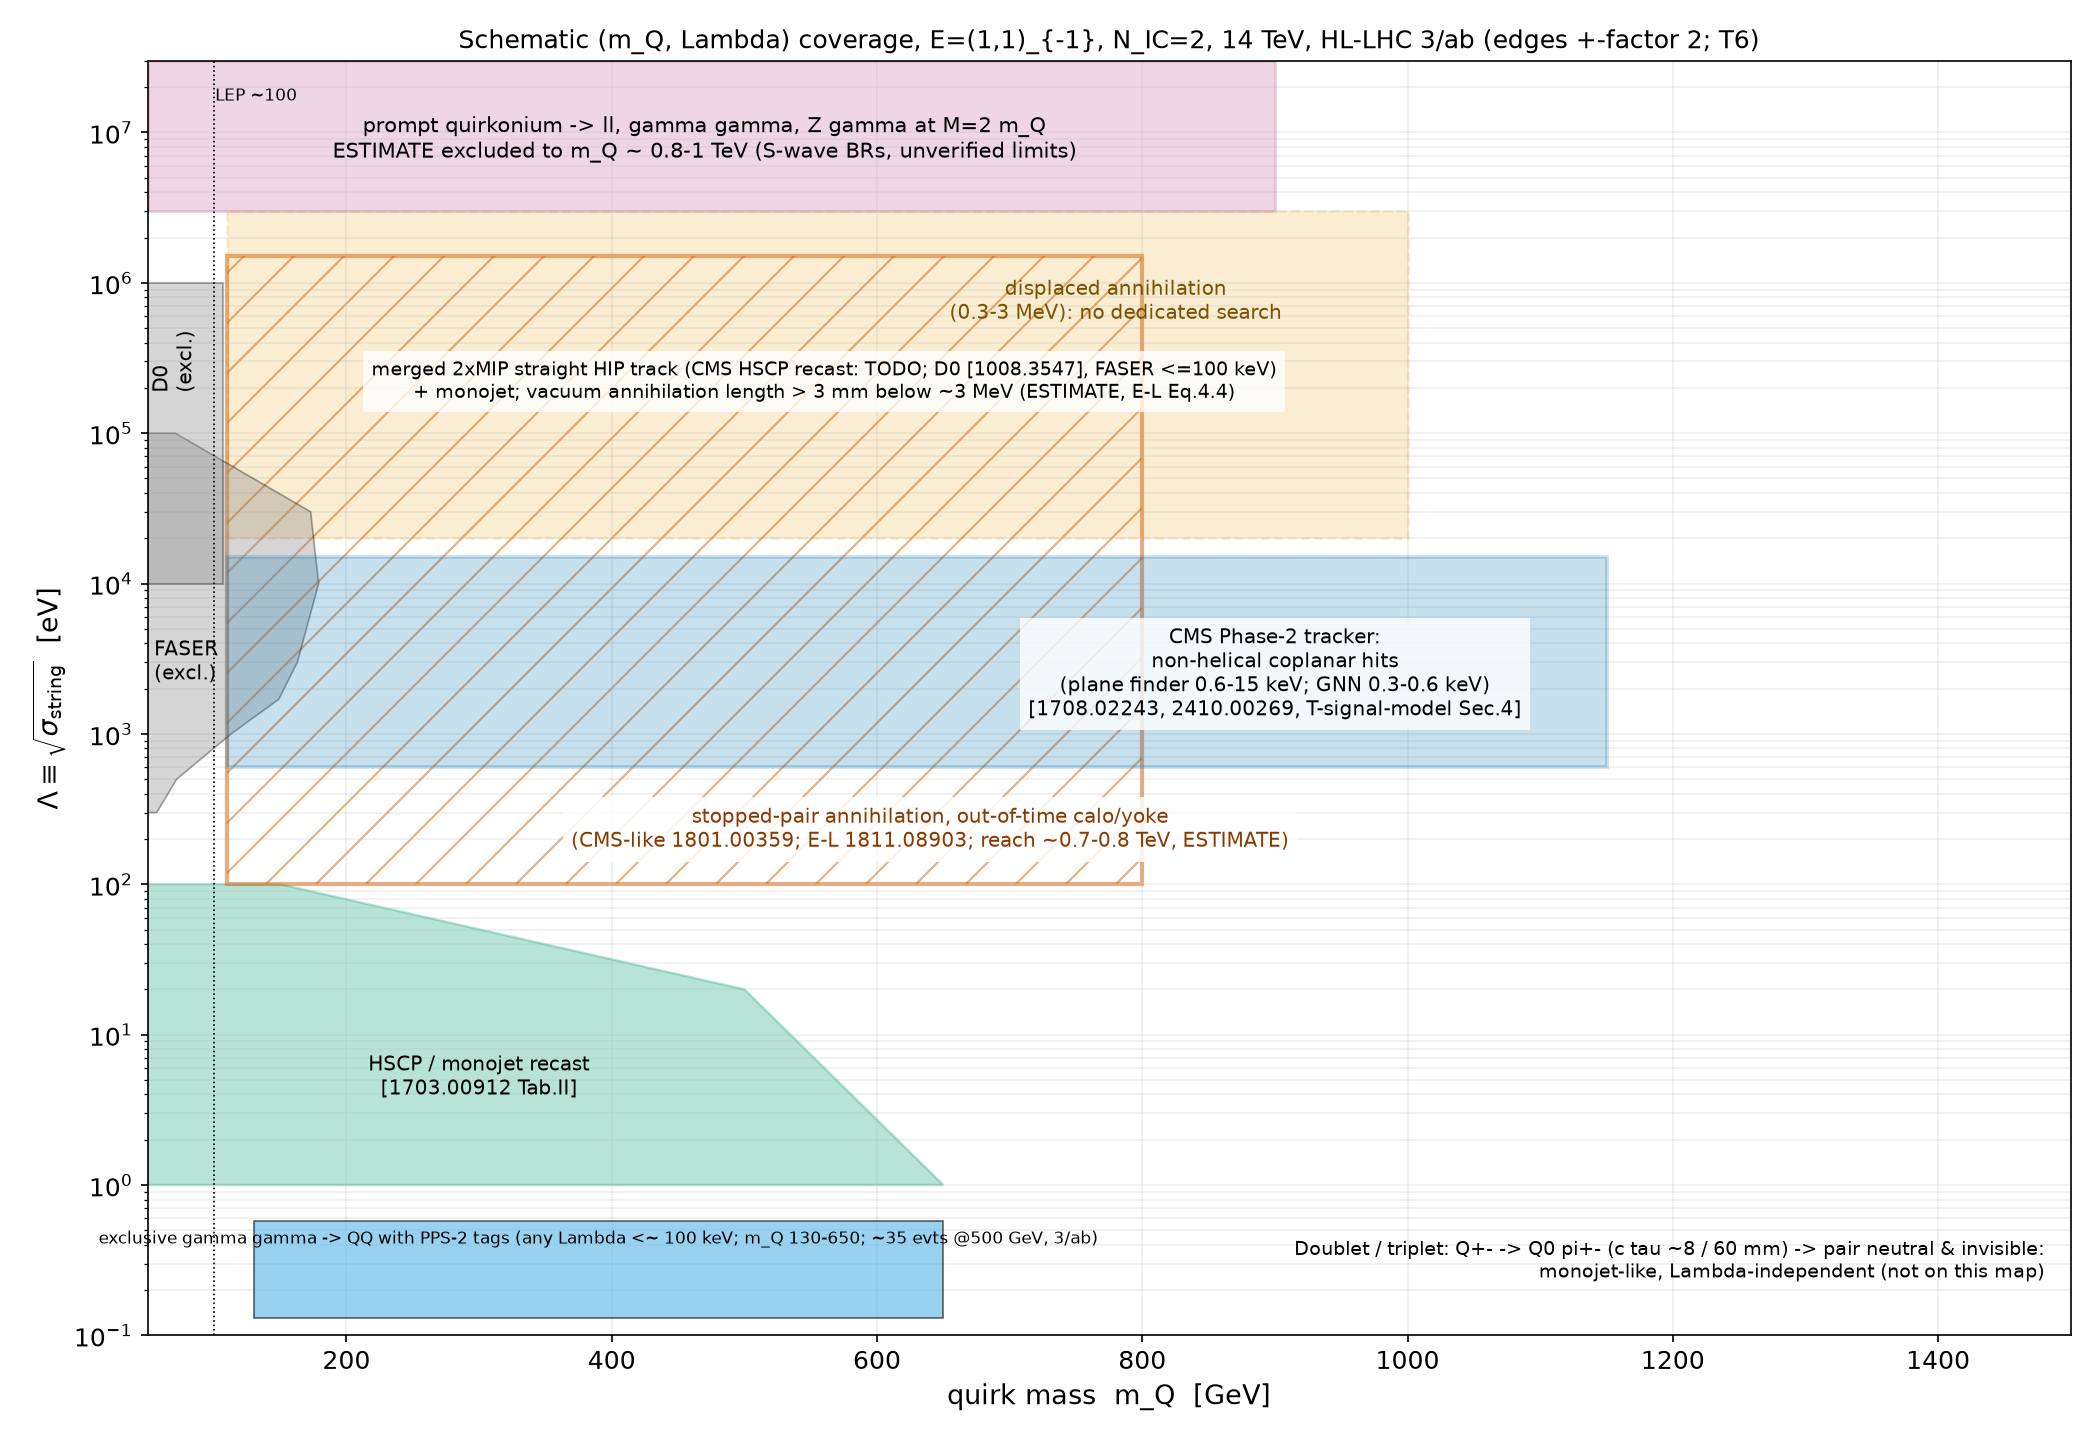
\includegraphics[angle=90,height=0.70\textheight]{figures/T6_coverage_rep.png}
\caption{\textbf{Schematic coverage map of the $(\mQ,\Lambda)$ plane by T6} \src{T6; \file{code/T6_coverage.py}; \EST{}, edges $\pm$ factor 2; drawn before the reviews}. \textcolor{bad}{\textbf{Two labels are superseded}}: the stopped-pair box reach ``$\sim0.7$--0.8\,TeV'' is now 0.3--0.55\,TeV (EB+HB, HL-LHC) or $\approx0.15$--0.35\,TeV (Run 2+3) (S-8); and the merged pair is a 9--21$\times$ MIP object at CMS, not ``2$\times$MIP'' (S-10). The tracker window 0.6--15\,keV is the pre-track value (truth-level lower edge now 0.45--0.7\,keV), and the prompt-resonance region is an \UNV{} reading of existing limits. Also: the displaced-annihilation band is labelled 0.3--3\,MeV (v4: 0.1--3\,MeV); the stopped-pair box extends in $\Lambda$ far beyond the range where $f_{\rm stop}$ was computed (0.3--3\,keV); and exclusive $\gamma\gamma$ + PPS is drawn as coverage although it was killed as a discovery channel (post-discovery mass handle only). Fonts enlarged and the page rotated for this report; content unchanged.}\label{fig:T6}
\end{figure}

% ======================================================================
\section{Publishable outputs}\label{sec:papers}
A CMS member may write phenomenology papers, but none may use CMS-internal information (Phase-2 material, PU-200 MET resolution, detector timing must come from public TDRs or generic detectors); confirm with the conveners (OQ Q2, Q13).
{\footnotesize
\begin{longtable}{@{}L{0.6cm}L{3.1cm}L{4.1cm}L{3.8cm}L{1.3cm}L{2.6cm}@{}}
\caption{Paper candidates (synthesis \S5).}\label{tab:papers}\\
\toprule ID & Working title & Available now & Missing for publication & Effort & Value / novelty\\\midrule\endfirsthead
\toprule ID & Working title & Available now & Missing for publication & Effort & Value / novelty\\\midrule\endhead
\bottomrule\endfoot
P1 & Quirk-pair trajectories in a solenoid: exact string dynamics, crossing-generated plane thickness, and multiple scattering & $\Ds_B\propto\Lambda^{-1.6\ldots-2.0}$; $B\ln(1/B)$ mechanism (two solvers); MS floor and $\sqrt{x/X_0}$; resolution effect; causal validated ($\le1\%$); converged Li $-3\ldots-35\%$ ($\gst$); Li at printed step $\times0.8$--20; lab slices $\times1.5$--75 & analytic crossing impulse ($c\approx0.10$); Athena C++ on common events; independent solver with MS; $\ge200$ events/point with public material; full credits (Li App.C and \S V; Athena authors J.~Black, T.~Nelson et al.; Artru/Lund; Kang--Luty; Knapen; Sha; FASER); contact Athena/FASER and Knapen--Papucci & 3--5 wk & \textbf{Medium.} Novel: $B\ln(1/B)$ mechanism, $\gst$-dependent comparison and convergence requirements, central-detector MS, causal thickness numbers. \emph{Not} novel: the causal string; qualitative $\mQ$ independence, $\sim\Lambda^{-2}$, $\propto q$. Risk: reads as a validation note; lead with physics; claim ``public codes'' only\\
P2 & Measuring the quirk mass and string tension: a degeneracy theorem and the recoil & theorem; CRB tables; MET alignment; predictive $\chi^2$; linearity/aliasing & a real fit (Gauss--Newton or SBI) with assignment ambiguity, PU hits, MS; public MET assumptions; could merge into P1 & 3--6 wk after P1 & Medium-high: first answer to a problem open since 2017 [1708.02243 \S IV]\\
P3 & Stopped quirks at the HL-LHC & causal $f_{\rm stop}$, dissipation times, BRs, revised reach, ISR coincidence & 3D geometry and field map; $\Lambda$ up to 1\,MeV; HL-LHC filling scheme; energy-threshold background & 1--2 mo & Medium-low (0.3--0.55\,TeV EB+HB); extends E--L's 300\fbinv\ projections to 3\abinv\\
P4 & Cosmology of the mesoscopic quirk window (note) & $T_{\rm RH,max}$ map, $T^{21/4}$, $\times2.2$, $\Delta N_{\rm eff}$ & resolve $\times2.2$ with the authors; re-derive the dim-8 matrix element & 2--3 wk & Low-medium; better as a comment\\
P5 & GUT-motivated doublet quirks: invisible pairs and monojet limits & ladder strips, $c\tau$, rates & the monojet recast; coloured-$D$ limits & 2--4 wk & Low-medium\\
P6 & Stopped quirks in full Run-2+3 data: an update of the out-of-time recast (better CMS-internal) & $f_{\rm stop}$, delays, ${\rm BR}_{\rm vis}$, reach estimate & E--L method with Stage-3 effective luminosity; selection efficiency for $2\mQ$ deposits; $f_{\rm stop}(\Lambda)$ to $\gtrsim100\keV$; threshold background & 2--4 wk & Low-medium as a paper; medium as a CMS-internal result ($\approx0.15$--0.35\,TeV; above FASER/D0 at $\Lambda\lesssim1.5\keV$ even with a 2016-like background)\\
\end{longtable}
}
Recommended order: \textbf{P6} as a CMS-internal update (a stronger limit, no dependency), then \textbf{P1} (needs the analytic crossing theory), then \textbf{P2} (reuses P1's code).

% ======================================================================
\needspace{14\baselineskip}
\section{Killed ideas}\label{sec:killed}
{\footnotesize
\begin{longtable}{@{}L{5.6cm}L{7.6cm}L{3.0cm}@{}}
\caption{Ideas that do not survive, with the number that kills them (synthesis \S6).}\label{tab:killed}\\
\toprule Idea & Killing number & Source\\\midrule\endfirsthead
\toprule Idea & Killing number & Source\\\midrule\endhead
\bottomrule\endfoot
``Published central-detector trajectory models are wrong at O(1)'' (v1 S-1 headline) & literal Li, converged: $\Ds$/causal 0.84--1.05 at $\gst=1.28$ (0.65--0.97 medians over $\gst=1.05$--3); labSS/Li 1.6--73; Li + MS no fake mm & R1 A-1; F1; S-1\\
Lab-time-slice straight string as a propagator & $\times1.5$--75 in $\Ds$ (median $\approx9$); 140--570\um\ frame dependence; $-1.6$\,MeV/crossing; fake 0.2--21\,mm with MS & T2 \S5.1; T3 \S3.1\\
Li-type Euler integration at the printed step & $\times0.8$--20 in $\Ds$, OT hits 6--250\,mm off & R1; S-1\\
Plane precession in B as a $\Lambda$ meter & 3--18\,$\mu$rad (0.6--1\,keV), $\le0.3\,\mu$rad ($\ge3\keV$) $<$ MS 4.5--10\,$\mu$rad (Knapen bounded $\Delta\phi\lesssim10^{-3}$ [1708.02243 Eq.8--9]) & T3 \S4.2\\
Thickness $\propto\mQ/\Lambda^4$ as a $\Lambda$ or $\mQ$ meter & B term $\propto qBR/\Lambda^2$ ($\mQ$-independent); formula $\times7$--50 off at 3\,keV & T3; T4; X-2\\
dE/dx or MTD timing as a mass handle & measure $\beta\gamma$ only; IT dE/dx changes $\sigma(\mQ)$ by 0\% & T4 \S8\\
``Positions alone measure $\mQ$ and $\Lambda$'' & vacuum $\ln\sigma$ Fisher column $\le3\times10^{-7}$ of the largest & T4 \S3.1\\
Vacuum + first-order-B analytic fit model & misses 30--45\% of the B effect (\VER{}) & T4; S; R1\\
Kalman filter with a two-point state & linearity window $\le0.1$ cycle; 3--300 oscillations between layers at $\ge3\keV$ & T4 \S2.4\\
Truth-level 3D $\Ds$ as reconstructed observable & 2S $\sigma_n\approx8$\,mm, PS 0.25\,mm; event-level 23--30\um & S-2\\
Midpoint of two quirk hits as a ``CM track'' & deviates by 35--50\% of the half-separation & T4 \S6\\
Lab-frame ``simultaneity problem'' in vacuum & all methods agree to $\le2\times10^{-8}\lmax$ & T2 \S2.1\\
Fixed-$\hat s$ approximation & no transverse restoring force once $F_{\rm ext}\ne0$ (Li et al.\ noted it) & T2 \S9\\
Rotating component from DY spin & $J/(p^*\lmax)\approx3\times10^{-17}$ & T2 \S4\\
Capture or annihilation at crossings (CMS) & $J\ge10^6\hbar$ from the first crossing in 3.8\,T & T2 \S5.3\\
Relativistic yo-yo formula & $\gst\le2.0$--2.5 at the 84th percentile; formula $\times3$--6 off & T2 \S2.4\\
Quantum spreading, roughening, Larmor, perturbative glueball radiation & 0.5\,nm; 5\,\AA; $1.5\times10^{-8}$\,eV$(\Lambda/\keV)^4$ per crossing; $\sim10^{-20}\Lambda$ & T2 \S6\\
L\"uscher corrections, string breaking, quirk--quirk Coulomb & $10^{-8}$ at 1\um; $\exp(-3\times10^{16})$; $3\times10^{-10}$ & T5 \S7\\
$\varepsilon$ inside the CMS tracker & $\lesssim0.1$\,GeV deposited & T2 \S6.3\\
Delta rays, straggling as thickness sources & recoil $\approx0.2$\,MeV $\ll$ 5--15\,MeV MS kick & T3 \S11\\
B-field non-uniformity in the barrel & $B_r/B_0\le0.9\%$ $\Rightarrow\lesssim1$--2\% & T3 \S4.3\\
Doublet/triplet charged members as tracker quirks & survival to 3\,cm $\le0.2\%$ (doublet) & T3 \S5; T6\\
Internal motion enhancing the merged-pair dE/dx & 0.75--0.90 $\times$ two HSCPs & T3 \S8\\
Hit-level dE/dx phase tagging & only 4 IT layers measure charge (Phase 2) & T3 \S8\\
Inelastic $\gamma\gamma$ as a boost; exclusive $\gamma\gamma$+PPS for discovery & +4.0--4.2\%; 35 events at 500\,GeV & T6\\
Spin as an acceptance driver & $\le25\%$ & T6\\
Cosmic-ray, beam-dump, MoEDAL, MATHUSLA/CODEX-b/ANUBIS/FACET & kinematics / stopping in shielding & T6\\
Stellar cooling; $Z\to g'g'$; light-by-light & $\mQ>1.5\GeV$; BR $\sim10^{-12}$; $(\Lambda/\mQ)^4$ & T1 \S3\\
BBN/CMB/$\gamma$-ray glueball-decay bounds; CMB-S4 $\Delta N_{\rm eff}$ & $\tau\ge10^{35}$\,s; $\Delta N_{\rm eff}\sim6\times10^{-4}$ & T1 \S3\\
SIDM recalibration; cannibalism as strengthening; Banks--Zaks keV; neutral naturalness keV & $\le\times1.6$; $\Lambda/\mQ\sim0.02$; $\sqs\approx2$--40\,GeV & T1\\
Electron stripping in the tracker; net-charged pairs as a benchmark & needs $\beta\lesssim0.01$; no benchmark & T5 \S7; T3 \S5\\
\end{longtable}
}

% ======================================================================
\needspace{14\baselineskip}
\section{Review history}\label{sec:review}
JFC vocabulary: \catA{} = wrong or misleading claim (or would mislead the experimental track); \catB{} = weakens a result or missing credit, must fix; \catC{} = polish. ITERATE = fix and re-review; PASS = accept.

\subsection{Rounds and verdicts}
{\footnotesize
\begin{longtable}{@{}L{1.9cm}L{2.0cm}L{6.2cm}L{6.0cm}@{}}
\caption{Review rounds (synthesis \S10; review files).}\label{tab:rounds}\\
\toprule Round & Verdict & A items and key B items & How fixed\\\midrule\endfirsthead
\toprule Round & Verdict & A items and key B items & How fixed\\\midrule\endhead
\bottomrule\endfoot
R1 critical (Opus; own NG solver + literal Li) & ITERATE 3\,A/8\,B/9\,C & \catA-1 S-1 numbers describe T2's labSS, not Li et al.\ (literal Li, converged: $-16\%\ldots+4\%$; with MS no fake mm). \catA-2 downstream advice would mislead Phase~2. \catA-3 ``35/35 PASS'' never tested the S-1 premise. \catB-1 ``exact'' = classical NG; \catB-2 all efficiencies truth level, resolution $\approx$ MS floor; \catB-3 $\times7$--50 already in Li App.C; \catB-4 material unverified; \catB-5 1\%/0.5\% below the MET-scale floor; \catB-6 stopped-pair live fraction and background; \catB-7 ranking; \catB-8 T2's $\Lambda^{-2.5}$ & v2: headline \WD{}; S-1 rewritten around four statements; \file{F1_standin.py} (labSS/Li 1.6--73), \file{F1_li_phase.py}; erratum boxes in T2/T3; \S3.0 ``what the checks did not test''; \file{F1_smear.py} (per-hit $\sigma_n$); Li App.C credited; 1--3\%/0.5--1.5\% headline; \file{F1_stopped.py} (0.3--0.55\,TeV)\\
R1 constructive (Sonnet) & 3\,A/11\,B/12\,C & \catA1 headline vs small effect on reach; \catA2 no ``no new exclusion'' statement, \UNV{} next to \VER{}; \catA3 MET-strip $\times13$--34 vs real background. B: consolidated $\Lambda$ answer, oscillation-length box, PU vertex, HLT, Run-3 table, ML features, SBI, recast table, S-7 idealised, P1 novelty, glossary & bottom-line paragraph; VERIFIED/UNVERIFIED table; Box~A, Box~B; \S4.5 recast table; \S4.6 Run-3 table; S-18 notes; glossary\\
R2 fresh (Opus) & ITERATE 1\,A/4\,B/9\,C & \catA1 stopped-pair recast framed as novel (``first LHC limit''), but Evans--Luty already recast 1801.00359 for this benchmark. \catB1 ``Li $\approx15\%$ low'' measured at one $\gst$: 3\% at 1.05, 30--35\% at 2--3. \catB2 existing $E$ exclusions missing. \catB3 Run-2+3 headline used rejected assumptions. \catB4 smeared vs truth edge compared at unequal background & v3: E--L credited, item reframed as an update; $\gst$-dependent deficit everywhere, event-by-event validation in $\gst$ bins; Farina--Low, E--L, D0, FASER added; 0.15--0.35\,TeV; no edge-shift claim\\
R3 fresh (Opus) & ITERATE 0\,A/6\,B/9\,C & \catB1 FASER limit is $\Lambda$-dependent (C-shaped), so ``beats FASER only if $B\lesssim O(10)$'' was wrong at the $\Lambda$ edges. \catB2--B6 missing credit: Li \S V/Fig.4; Knapen \S IV $\Delta\phi$; Sha \S V $\chi^2$; Athena G4 EM material; 2512.20696 reheating headline & v4: FASER per $\Lambda$; all credits added; novelty narrowed; 2108.06748 \S5 statement added\\
R4 fresh (Sonnet) & \textbf{PASS} 0\,A/0\,B/7\,C & housekeeping; exec-summary credit and $\gst$ qualifier; ``near 100\,keV'' flagged extrapolated; ``refutes'' softened to ``not supported''; FASER readings \UNV{} until HEPData & applied in place (\S10.4); track closed\\
\end{longtable}
}

\subsection{What the withdrawn v1 claim looked like}
\begin{figure}[H]\centering
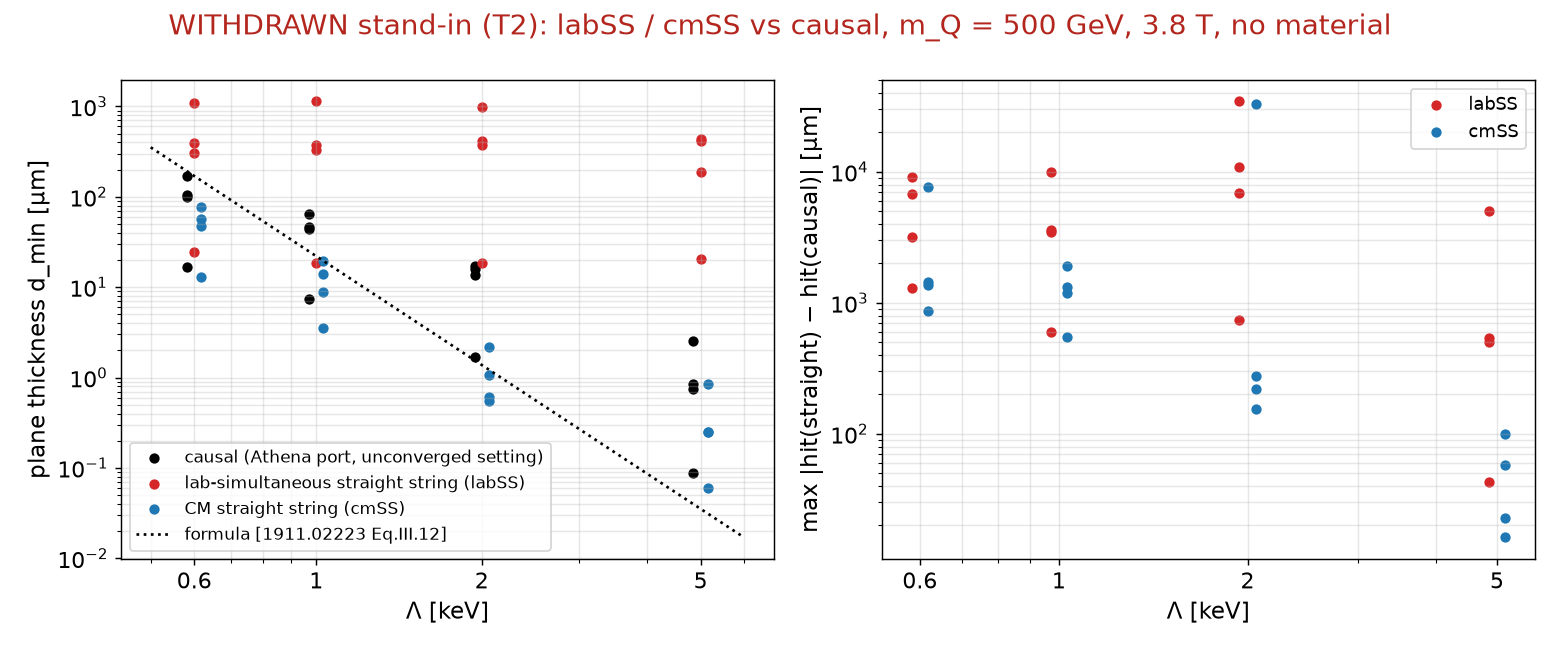
\includegraphics[width=0.92\textwidth]{figures/T2_string_methods_B_rep.png}
\caption{\textcolor{bad}{\textbf{WITHDRAWN stand-in; shown only to document the error.}} T2's comparison of string prescriptions in 3.8\,T without material ($\mQ=500\GeV$, $\gst=1.28$, 4 events per $\Lambda$) \src{T2 \S5.1 item 4; \file{code/T2_string_methods_B.py}}. Red: the lab-simultaneous straight string (labSS); blue: the CM straight string (cmSS); black: the causal string at an unconverged setting (up to 25\% off the converged causal values). Neither labSS nor cmSS is the published Li et al.\ algorithm, and no paper used them; this plot is the origin of the v1 numbers ``$\times0.04$--60 in thickness, 0.2--35\,mm in OT hits''. The converged literal Li integrator lies within 3--35\% of the causal string in the median (single events $-47\%\ldots+36\%$; Table~\ref{tab:S1}). Re-plotted from \file{figures/T2_string_methods_B.npy} with readable ticks.}\label{fig:withdrawn}
\end{figure}

\needspace{16\baselineskip}
\subsection{Where the errors came from}
{\small
\begin{longtable}{@{}L{3.3cm}L{7.2cm}L{5.8cm}@{}}
\caption{Classification of the errors found by the reviews.}\label{tab:errclass}\\
\toprule Origin & Instances & Lesson\\\midrule\endfirsthead
\bottomrule\endfoot
Stand-in implementation & labSS/cmSS used for ``Li et al.''; validated only in vacuum, where it coincides with Li (R1 A-1, A-2) & implement the published algorithm literally before criticising it; validate where the effect lives (here: with $F_{\rm ext}\ne0$)\\
Untested premise & spot checks re-derived numbers but never compared a published integrator or an independent solver (R1 A-3) & state what a check does \emph{not} test\\
Lost or missing credit & Evans--Luty recast (R2 A1; T6 knew it); Li \S V, Knapen \S IV, Sha \S V, Athena G4 EM, 2512.20696 (R3 B2--B6) & audit every ``new'' against the primary texts (done in R3, verified in R4)\\
Overclaiming / generalising & ``15\%'' from one $\gst$ (R2 B1); edge shift at unequal background (R2 B4); 1\%/0.5\% below the floor (R1 B-5); $\times13$--34 vs random planes only (R1-k A3); idealised $\times20$--100 (R1-k B9) & quote the kinematic point and the floor with every headline\\
Unconverged numerics & T2's $\Lambda^{-2.5}$ with an unconverged causal column (R1 B-8); 0.65\,TeV reach with long-delay live fraction (R1 B-6) & convergence and acceptance tests before scaling laws and reaches\\
Misreading a figure & FASER contour read as flat (R3 B1) & use HEPData; it was in the project already (Section~\ref{sec:owndisc})\\
\end{longtable}
}

\subsection{Disagreements that remained}
S-1 stays at rank 1 (R1 B-7 suggested demoting it), but re-scoped as ``validated production propagator'', the most actionable item. Declared as not done after all rounds: the Li covariance re-test with the literal prescription; an independent string solver with MS; Li convergence at 5\,keV; PU and alignment in the smearing study; the Athena C++ comparison; the HL-LHC trigger fraction with E--L's method; $\gst$ dependence at higher statistics.

% ======================================================================
\section{Residual uncertainties, next steps and decisions}\label{sec:next}
\subsection{What remains \UNV{} or idealised}
\begin{enumerate}
\item \textbf{Phase-2 material per layer} (most important): $\approx19\%\,X_0$ at $\eta=0$ is a reconstruction (Phase-2 TDR could not be opened); the per-layer split (PS 2.5\%, 2S 1.8\%, IT 1.2\%) is a guess; IT material only at $|z|<20$\,cm. Drives the MS floor, $f_{\rm stop}$ and S-12.
\item \textbf{Detector resolution and readout}: pitch/$\sqrt{12}$ guesses (IT $25\times100\,\mu$m$^2$, PS $100\um\times1.5$\,mm, 2S $90\um\times5$\,cm); no charge sharing, alignment, inefficiency, PU hits.
\item \textbf{String model}: not confirmed against the Athena C++ (G4 geometry, \texttt{DistChord()}$=0$); not confirmed with MS by an independent string solver; classical-NG validity at near-miss crossings for $\Lambda\gtrsim10$--20\,keV; hit recorder misses grazing double crossings.
\item \textbf{Small MC statistics}: thickness 60 events/point ($\le3\keV$), 24 at 10\,keV, 12 at 30\,keV; Fisher 16; Li comparisons 5--24 per point; medians carry 10--30\% statistical uncertainty.
\item \textbf{Measurement idealisations}: local CRB, known assignment, no PU, thin scatterers.
\item \textbf{Experimental inputs}: PU-200 PUPPI MET resolution and the 1--3\% scale; IT ToT range; OT stub windows; BTL $\sigma_t$ and TOFHIR double hits; HL-LHC filling scheme and empty-BX livetime; stopped-particle background; Run-3 parameters.
\item \textbf{Kinematics}: LO DY+ISR toy with $\pTQQ>200\GeV$; $f_{\rm stop}$ depends on an assumed low-$p_T$ spectrum ($\times2$).
\item \textbf{External limits not opened}: ATLAS dilepton/diphoton at 1.4--2\,TeV; monojet/compressed EW; multi-charge; PPS-2 schedule; any Run-2 update of 1801.00359.
\item \textbf{Cosmology}: freeze-in matrix element taken from 2512.20696 Eq.26 without re-derivation; the $\times2.2$ is unexplained.
\item \textbf{$\varepsilon$ model and GUT ladder}: heuristic $\varepsilon(b)$; ladder running $\times2$--4.
\item \textbf{Code not inspected}: Knapen--Papucci; Sha et al.\ propagator.
\end{enumerate}

\needspace{14\baselineskip}
\subsection{Recommended next steps (ordered)}
{\small
\begin{longtable}{@{}L{0.5cm}L{6.0cm}L{5.0cm}L{1.9cm}L{2.4cm}@{}}
\caption{Next steps (synthesis \S8, ordered).}\label{tab:next}\\
\toprule \# & Step & Why & Effort & CMS access?\\\midrule\endfirsthead
\bottomrule\endfoot
0 & \emph{Done:} cache, PDF grid and Athena snapshot copied to \file{theory_track/data/}, code defaults repointed (Section~\ref{sec:reading}) & reproducibility & -- & no\\
1 & Do first: (a) hand \file{T3_causal.py} to Phase~2 as W3 with the two-roots-per-chord fix; (b) S-9 looper-killer exemption in the CMS port; (c) define the resolution-aware coplanarity test with the experimental team; (d) ask Knapen--Papucci and Sha et al.\ for their string prescription and step (or code) & immediate value; removes risks & days & (c) yes\\
2 & Run-2(+3) update of Evans--Luty's out-of-time recast (P6, CMS-internal), with their trigger-fraction method or 1801.00359 Stage~3, $f_{\rm stop}(\Lambda)$ to $\gtrsim100\keV$, energy-threshold background; use FASER HEPData values & most likely route to a stronger limit (0.15--0.35\,TeV) & 2--4 wk & optional\\
3 & Real Phase-2 material and resolution; re-run \file{T3_ms_thickness.py} and \file{F1_smear.py} at $\ge200$ events/point; efficiency curves for a resolution-aware finder & the window and $\Ds$ optimisation at PU 200 need them & 3--5 days & yes\\
4 & Analytic crossing theory ($c\approx0.10$) & P1 content; replaces the formula & 1--2 wk & no\\
5 & Athena C++ standalone on $\sim10$ common events; extend R1's solver to MS & last validation of the production model & 1 wk & no\\
6 & Write P1 & after 4--5 & 3--5 wk & no\\
7 & Measurement demonstration (Gauss--Newton and/or SBI) with assignment ambiguity, PU hits, alignment & P2; realistic S-7 rejection & 3--4 wk & partly\\
8 & MET-strip gain on real backgrounds & S-5 must not enter a background estimate unmeasured & experimental & yes\\
9 & Doublet monojet recast; GUT-ladder lines & S-14 & $\sim$1 wk & no\\
10 & $|q|=2$ window with the causal string & S-17 & 2--3 days & no\\
11 & Cosmology note (contact 2512.20696 authors) & S-15 & 1--2 wk, optional & no\\
12 & $\varepsilon(b)$ and $J$ random walk for FASER & S-19, low CMS value & weeks & no\\
\end{longtable}
}
Hand-offs that are not theory work: OI-1 timing (S-6), MET-alignment implementation and its real-background gain (S-5), PU-200 random-plane background, PU-vertex association and an L1 $\phi$-road (S-18), the HSCP recast (S-10).

\subsection{Decisions for the user}\label{sec:decisions}
\begin{enumerate}
\item \textbf{Apply the document changes?} Which rows of Section~\ref{sec:mods} (a1)--(a4) to apply to STRATEGY, SAMPLE\_REQUIREMENTS, theory\_signal\_model and OPEN\_QUESTIONS (the ``must'' rows change numbers used downstream: timing medians, window, MIP multiple, string model, validation items V2--V5, MaxSteps, MS in Geant4).
\item \textbf{Production propagator}: adopt \file{T3_causal.py} as the Phase-2 W3 starting point and the GNN truth generator, and require any external sample (Zenodo/Sha) to be validated against it.
\item \textbf{Stopped-pair update (P6)}: launch it now as a CMS-internal Run-2+3 task (the only route identified to a stronger limit on this benchmark)?
\item \textbf{CMS-internal inputs}: pull the Phase-2 $x/X_0(\eta)$, pitches and alignment residuals, PUPPI MET resolution at PU 200, and check for a Run-2/3 update of the stopped-particle search.
\item \textbf{Contacts}: Knapen--Papucci and Sha et al.\ (code prescription); Athena/FASER authors (MaxSteps at 100\,keV; C++ comparison); 2512.20696 authors ($\times2.2$, $T^{21/4}$) before any public statement.
\item \textbf{Benchmarks}: OQ Q4 as $E$ + $\tilde E$ without the two $L$ points; whether to add a $|q|=2$ point.
\item \textbf{Papers}: whether to invest 3--5 weeks in P1 (and then P2), given the policy on CMS-internal information.
\end{enumerate}

% ======================================================================
\appendix
\section{Bibliography}\label{app:bib}
Papers cited in this report (as used by the track; tags in the text such as [1911.02223 Eq.III.12] refer to these arXiv numbers). Where the full title was not checked, the entry describes the content used.
\begingroup\small
\renewcommand{\section}[2]{}
\begin{thebibliography}{99}\setlength{\itemsep}{1pt}
\bibitem{KL} J.~Kang, M.~A.~Luty, \emph{Macroscopic Strings and `Quirks' at Colliders}, \arx{0805.4642} (labelled ``KLN'' in the track files, although the paper has two authors). Used: \S2.5 GUT ladder, \S3.2 straight string ``check by direct simulation'', \S4.1, \S5 annihilation (Eq.5.59), \S5.7 $\varepsilon$ extremes.
\bibitem{D0} D0 Collaboration, \emph{Search for New Fermions (`Quirks') at the Fermilab Tevatron Collider}, \arx{1008.3547}. Used: 107\,GeV limit; per-trajectory dE/dx ($\gtrsim15$\,MeV/cm).
\bibitem{Martin} S.~P.~Martin, \emph{Quirks in Supersymmetry with Gauge Coupling Unification}, \arx{1012.2072}. Used: Tab.I anchor of the SUSY-GUT ladder.
\bibitem{HKM} R.~Harnik, G.~D.~Kribs et al., \emph{Quirks at the Tevatron and Beyond}, \arx{1106.2569}. Pointer for $\beta$-decaying EW multiplets (abstract only).
\bibitem{FarinaLow} M.~Farina, M.~Low, \emph{Constraining Quirky Tracks with Conventional Searches}, \arx{1703.00912}. Used: Tab.II limits, 0\,T proposal.
\bibitem{Knapen} S.~Knapen, H.~K.~Lou et al., \emph{Tracking down Quirks at the Large Hadron Collider}, \arx{1708.02243}. Used: $\Ds$ definition (Eq.11), \S II string, \S IV $\Delta\phi$ cut and trajectory-fit remark, App.A dE/dx, Eq.8--9, Fig.6 reach.
\bibitem{EvansLuty} J.~A.~Evans, M.~A.~Luty, \emph{Stopping Quirks at the LHC}, \arx{1811.08903}. Used: recast of CMS 1801.00359, $f_{\rm stop}$, trigger fractions (Figs.3--5), Eq.4.3--4.4, App.B, \S2 retardation remark, \S5--6.
\bibitem{LiLi} J.~Li, T.~Li et al., \emph{Uncovering quirk signal via energy loss inside tracker}, \arx{1911.02223}. Used: Eq.III.6--10 (Li method, step bound), Eq.III.12 (thickness formula), App.A reach, Sec.V.
\bibitem{traj} J.~Li, T.~Li et al., \emph{The quirk trajectory}, \arx{2002.07503}. Used: Eq.II.4--8, \S IV $n_T$, \S V/Fig.4 thickness, \S V.A $q$-linearity, \S VIII/Fig.6 fixed $\hat s$, App.C/Fig.8 formula vs numerics, Tab.I hits per layer.
\bibitem{LiPei} J.~Li, J.~Pei et al., \emph{The quirk signal at FASER and FASER 2}, \arx{2108.06748}. Used: \S4.1 ionisation torque, \S4.3 Eq.4.18, \S5 measurement statement.
\bibitem{FarDet} J.~Li, X.~Liao et al., \emph{Detection prospects of long-lived quirk pairs at the LHC far detectors}, \arx{2311.15486}. Used: K-factors.
\bibitem{Feng} J.~L.~Feng, J.~Li et al., \emph{Discovering quirks through timing at FASER and future forward experiments at the LHC}, \arx{2404.13814}. Used: $\varepsilon$ ranges, length shorthand, K-factors.
\bibitem{Sha} Q.~Sha, D.~Murnane et al., \emph{Learning to reconstruct quirky tracks}, \arx{2410.00269}. Used: \S III propagator, \S V quirk vs helix $\chi^2$; samples on Zenodo 17941765.
\bibitem{Forsyth} \emph{Visible collider signals of natural quirks}, \arx{2504.02940}. Used: $\sigma=3.6\Lambda'^2$ convention.
\bibitem{Condren} L.~Condren, D.~Whiteson, \emph{Finding unexpected nonhelical tracks}, \arx{2509.08878}.
\bibitem{cool} P.~Asadi, G.~D.~Kribs, M.~A.~Luty, \emph{Quirks live in cool universes}, \arx{2512.20696}. Used: abstract, Eq.1, \S2, Eq.4--5, 11, 19, 26, \S4 ($T_{\rm RH}\lesssim\mQ/25$, $T^7$ scaling), Fig.4, App.B.
\bibitem{LHCb} X.~Cid Vidal et al., \emph{Searching for quirks at LHCb}, \arx{2601.09023}.
\bibitem{Review} \emph{Rich Phenomenology from Simple Ingredients: A Review of Confining Dark Sectors}, \arx{2606.30760}.
\bibitem{FASER} FASER Collaboration, \emph{First Search for Quirks at the LHC with FASER}, \arx{2607.26195}; HEPData ins3184325. Used: abstract, p.3 ISR reweighting, App.A (Geant4 EM processes), Fig.5 limits.
\bibitem{stopped} CMS Collaboration, search for stopped long-lived particles (2015--16 data), \arx{1801.00359}. Used: Sec.3, 3.2, 8, Tab.4.
\bibitem{ATLASstopped} ATLAS Collaboration, search for stopped long-lived particles, \arx{2104.03050}.
\bibitem{HSCP} CMS Collaboration, search for heavy stable charged particles with dE/dx, \arx{2410.09164}.
\bibitem{multi} ATLAS Collaboration, search for multi-charged long-lived particles, \arx{2303.13613}.
\bibitem{dilep} ATLAS dilepton resonance search, \arx{1903.06248}; diphoton resonance search, \arx{2102.13405} (limit readings \UNV{}).
\bibitem{latt1} Lattice SU($N$) deconfinement temperatures in units of $\sqs$ (Tab.6), \arx{hep-lat/0307017}.
\bibitem{Teper} M.~Teper, SU($N$) gauge theories review, $T_c/\sqs=0.597+0.45/N^2$ (Eq.33), \arx{0912.3339}.
\bibitem{latt2} Large-$N$ $T_c/\sqs$ (Eq.12), \arx{1202.6684}.
\bibitem{latt3} SU($N$) glueball masses and $\Lambda_{\overline{\rm MS}}/\sqs$ (Tab.15, 31; Eq.20--22), \arx{2106.00364}.
\bibitem{NN} Neutral-naturalness conventions ($m_0=6.8\Lambda_{\overline{\rm MS}}$), \arx{1501.05310}.
\bibitem{IT} Phase-2 Inner Tracker module material (Tab.1), \arx{2407.13721}.
\bibitem{P2mat} CMS Phase-2 tracker material ``substantially reduced'' (Sec.2, Fig.3), \arx{1912.02061}; Phase-1 tracker material $\approx0.4\,X_0$, \arx{1405.6569}.
\bibitem{ACT} ACT DR6 $N_{\rm eff}$, \arx{2503.14454} (abstract via web search).
\bibitem{PPS} Exclusive slepton production with proton tagging (EPA cross-check), \arx{1812.04886}.
\end{thebibliography}
\endgroup
\noindent Also used (non-arXiv): ATLAS Athena \file{Simulation/G4Extensions/Quirks} and \file{G4UserActions} (gitlab.cern.ch/atlas/athena, \texttt{main}, read 7 Oct 2026); GitHub \file{burzynski-lab/quirk-tracking}, \file{burzynski-lab/quirkviz}, \file{eliwelch17/PreFASERQuirkSim}, \file{shaqiyu/QuirkTracking-ML} (via the Phase-1 research reports); Zenodo 17941765; PDG Highland formula (recalled); CT18NLO and NNPDF3.1 luxQED PDF sets.

% ----------------------------------------------------------------------
\section{Code and figure inventory}\label{app:code}
All in \file{theory_track/code/}; run with \texttt{pixi run python code/<file>.py} from \file{theory_track/} unless noted. Status: \textbf{prod} = used for a number in synthesis v4; \textbf{lib} = imported by others; \textbf{check} = review or spot check; \textbf{test} = unit test; \textbf{superseded} = its headline output is withdrawn or replaced.
{\footnotesize
\begin{longtable}{@{}L{4.0cm}L{9.6cm}L{2.6cm}@{}}
\caption{Scripts (52 in \file{code/}, plus the report's figure script).}\label{tab:code}\\
\toprule Script & Purpose & Status\\\midrule\endfirsthead
\toprule Script & Purpose & Status\\\midrule\endhead
\bottomrule\endfoot
\file{T1_common.py} & lattice conversion factors, SU($N$) running, $g_*(T)$ & lib\\
\file{T1_lattice_conversions.py} & $\Lambda$ convention table; check vs Martin Tab.I & prod\\
\file{T1_running.py} & SUSY-GUT ladder strips, priors & prod\\
\file{T1_cosmo.py} & glueball lifetime, thermal history, freeze-in $T_{\rm RH,max}$ & prod\\
\file{T1_astro_collider.py} & stellar cooling, $Z\to g'g'$ (killed ideas) & prod\\
\file{T1_figure.py} & \file{T1_lambda_plane.png} & prod (figure)\\
\file{T2_propagator.py} & \texttt{ExactPair}, Li closed form, \texttt{CausalNullString} (Athena port); \texttt{LabStraightString} (labSS) & lib; labSS superseded\\
\file{T2_test_propagator.py} & 33 unit tests of the vacuum propagators & test\\
\file{T2_kinematics.py} & LO DY + ISR kinematics, $\lmax$, $N_{\rm osc}$; builds the shared cache (\file{data/cache/}) & prod\\
\file{T2_approx_errors.py} & accuracy of literature shorthands & prod\\
\file{T2_covariance_test.py} & Lorentz-covariance test of string prescriptions & check (straight columns: labSS/cmSS)\\
\file{T2_string_methods_B.py} & labSS/cmSS vs causal in 3.8\,T & \textbf{superseded} (v1 S-1)\\
\file{T2_transverse_linear.py} & linearised NG by characteristics vs causal and straight & check\\
\file{T2_crossing_missdist.py} & miss distance at crossings vs $1/\Lambda$ & prod (S-19)\\
\file{T3_propagator.py} & geometry, Phase-2 material, event sampling, Bethe; numba straight-string kernel & lib; kernel superseded\\
\file{T3_test_propagator.py} & validation of the numba kernel & test\\
\file{T3_causal.py} & \textbf{numba causal string with B, MS, dE/dx, straggling} & \textbf{prod (validated)}\\
\file{T3_ms_thickness.py}, \file{T3_ms_figure.py} & thickness with/without MS; figure & prod\\
\file{T3_precession.py} & plane precession (killed as $\Lambda$ meter) & prod\\
\file{T3_field.py} & solenoid fringe field estimate & prod\\
\file{T3_kick.py} & response to a single transverse kick & check\\
\file{T3_timing.py} & hit delays per layer, BTL & prod\\
\file{T3_stopping.py} & $f_{\rm stop}$ with the causal string & prod\\
\file{T3_dedx.py} & merged-pair dE/dx & prod\\
\file{T4_model.py} & 9-parameter causal hit model (kernel copy of the causal algorithm) & lib\\
\file{T4_fisher.py}, \file{T4_fisher_report.py} & Jacobians, Fisher, CRB tables and figure & prod\\
\file{T4_comb.py} & 1-D $\chi^2$ scans (linearity) & prod\\
\file{T4_met.py} & MET-strip alignment & prod\\
\file{T4_local.py} & stubs, seeding signatures & prod\\
\file{T5_census.py} & INSPIRE census (run from \file{stage2_C001_quirks/} with \texttt{python3}) & prod\\
\file{T5_estimates.py} & order-of-magnitude estimates (MS bound superseded by T3) & prod; MS item superseded\\
\file{T6_production.py}, \file{T6_table.py} & production cross sections (needs LHAPDF; separate conda Python) & prod\\
\file{T6_annihilation.py} & quirkonium BRs, annihilation length & prod\\
\file{T6_stopping.py} & dissipation time; yields (reach superseded by \file{F1_stopped.py}) & prod; reach superseded\\
\file{T6_coverage.py} & coverage map (two labels superseded) & figure\\
\file{S_spotchecks.py} & synthesis spot checks A--H & check\\
\file{S_Bnonlin.py}, \file{S_Bscan.py} & B non-linearity, $B\ln B$ shape & check\\
\file{S_msscale.py} & $\sqrt{x/X_0}$ scaling & check\\
\file{R1_conformal_ng.py} & \textbf{independent conformal-gauge NG solver} & check (reference)\\
\file{R1_li_literal.py} & literal Li et al.\ integrator & check\\
\file{R1_li_ms.py} & Li + thin-scatterer MS & check\\
\file{R1_Blinearity.py} & B linearity with the independent solver & check\\
\file{R2_li_checks.py} & Li vs causal vs $\gst$; finer steps at 3\,keV & check\\
\file{R3_lit_numbers.py} & literature figure readings; per-$\Lambda$ FASER comparison & check\\
\file{F1_standin.py} & labSS vs literal Li on the v1 events & check\\
\file{F1_li_phase.py} & residual Li hit differences (phase drift) & check\\
\file{F1_smear.py} & hit-resolution study & prod (S-2)\\
\file{F1_stopped.py} & stopped-pair reach with live fraction and background & prod (S-8)\\
\file{report/figures/regen_report_figures.py} & larger-font report copies of 9 figures (no new physics) & figure (report)\\
\end{longtable}
}

{\footnotesize
\begin{longtable}{@{}L{4.6cm}L{8.8cm}L{2.8cm}@{}}
\caption{Figures (14 PNG) and where they appear. Nine of them are shown in larger-font copies (\file{report/figures/*_rep.png}) made by \file{report/figures/regen_report_figures.py} from the original code or its saved data; the originals in \file{theory_track/figures/} are unchanged.}\label{tab:figs}\\
\toprule Figure & Content & Here\\\midrule\endfirsthead
\bottomrule\endfoot
\file{T1_lambda_plane.png} & $(\mQ,\Lambda)$ plane: GUT strips, freeze-in contours & Fig.~\ref{fig:T1}\\
\file{T2_lmax_distributions.png}, \file{T2_nosc_tracker.png} & $\lmax$ and $N_{\rm osc}$ distributions & Fig.~\ref{fig:osc1}\\
\file{T2_approx_errors.png}, \file{T2_isr_assumptions.png} & shorthand accuracy; ISR model & Fig.~\ref{fig:osc}\\
\file{T2_transverse_check.png} & causal vs straight for a pair at rest & Fig.~\ref{fig:transverse}\\
\file{T2_string_methods_B.png} & \WD{} labSS/cmSS comparison & Fig.~\ref{fig:withdrawn}\\
\file{T3_ms_thickness.png} & thickness vs $\Lambda$ (B, MS, B+MS) & Fig.~\ref{fig:T3ms}\\
\file{T3_timing.png} & hit delays & Fig.~\ref{fig:T3timing}\\
\file{T4_fisher_summary.png} & CRB resolutions & Fig.~\ref{fig:T4fisher}\\
\file{T4_comb.png} & linearity scans & Fig.~\ref{fig:T4comb}\\
\file{T4_met_alignment.png} & MET-strip alignment & Fig.~\ref{fig:T4met}\\
\file{T4_local.png} & stubs and local signatures & Fig.~\ref{fig:T4local}\\
\file{T6_coverage.png} & schematic coverage (two labels superseded) & Fig.~\ref{fig:T6}\\
\end{longtable}
}

% ----------------------------------------------------------------------
\section{Glossary}\label{app:gloss}
{\footnotesize
\begin{longtable}{@{}L{3.2cm}L{13.4cm}@{}}
\toprule Term & Meaning\\\midrule\endfirsthead
\toprule Term & Meaning\\\midrule\endhead
\bottomrule\endfoot
$\Lambda$ & $\sqs$, the square root of the string tension; $\sigma=50.68\,{\rm GeV/cm}\,(\Lambda/\keV)^2$\\
$\ell_0$, $\lmax$ & $\mQ/\sigma$; maximal CM separation $2(\gst-1)\ell_0$\\
$\gst$ & Lorentz factor of each quirk in the pair rest frame at production\\
$N_{\rm osc}$ & oscillations inside radius $R$: $\sigma R/(2\beta^*p_T)$\\
causal string & NG string with massive endpoints built from null segments (Athena; \file{T3_causal.py}); exact classical NG\\
Li method & CM-simultaneous straight string [1911.02223 Eq.III.6--10]\\
labSS / cmSS & lab-time-slice / extrapolated-CM straight strings written by T2; used by no paper\\
$\Ds$ & plane thickness (smallest-eigenvalue rms of hits about a plane through the PV)\\
$d$ (formula) & $1.16\um(\mQ/100\GeV)(\keV/\Lambda)^4(B/{\rm T})$ [1911.02223 Eq.III.12]\\
$b_{\rm odd}$ & miss distance at odd crossings $\approx3.5\um(\keV/\Lambda)^4$ in 3.8\,T\\
$x_B$ & T4's in-plane B displacement $\approx0.5\,qBR/\sigma$\\
$t_{\rm est}$ & thickness from smeared hits with a resolution-weighted plane fit\\
$\sigma_n$ & out-of-plane resolution of one hit\\
truth level & true hit positions, no resolution, known assignment, no PU\\
$f_{\rm stop}$ & fraction of pairs that stop in a given detector volume\\
$\varepsilon$ & glueball-emission probability per crossing\\
CRB & Cram\'er--Rao bound (Fisher-information resolution)\\
SBI & simulation-based inference\\
IT / OT; PS / 2S & Phase-2 Inner Tracker (pixels) / Outer Tracker; pixel-strip and strip-strip OT modules\\
BTL / MTD & Barrel Timing Layer of the MIP Timing Detector\\
EB, HB & ECAL and HCAL barrel\\
HSCP, MIP & heavy stable charged particle; minimum ionising particle\\
IC & infracolour, the new SU($\NIC$)\\
KLN, E--L, TH, STRAT, OQ, SREQ & Kang--Luty [0805.4642] (the track's label); Evans--Luty; \file{theory_signal_model.md}; STRATEGY\_DRAFT; OPEN\_QUESTIONS; SAMPLE\_REQUIREMENTS\\
S-$n$, X-$n$, T$n$, R$n$, F1, W & ranked gap; cross-report tension; investigator; reviewer; fix-pass executor; report writer\\
A / B / C; ITERATE / PASS & JFC review categories and verdicts\\
\EST{}, \UNV{}, \VER{}, \WD{} & own calculation; not checked against a primary source; checked independently; retracted claim\\
\end{longtable}
}
\end{document}
